\documentclass[twoside]{book}

% Packages required by doxygen
\usepackage{calc}
\usepackage{doxygen}
\usepackage{graphicx}
\usepackage[utf8]{inputenc}
\usepackage{makeidx}
\usepackage{multicol}
\usepackage{multirow}
\usepackage{textcomp}
\usepackage[table]{xcolor}

% Font selection
\usepackage[T1]{fontenc}
\usepackage{mathptmx}
\usepackage[scaled=.90]{helvet}
\usepackage{courier}
\usepackage{amssymb}
\usepackage{sectsty}
\renewcommand{\familydefault}{\sfdefault}
\allsectionsfont{%
  \fontseries{bc}\selectfont%
  \color{darkgray}%
}
\renewcommand{\DoxyLabelFont}{%
  \fontseries{bc}\selectfont%
  \color{darkgray}%
}

% Page & text layout
\usepackage{geometry}
\geometry{%
  a4paper,%
  top=2.5cm,%
  bottom=2.5cm,%
  left=2.5cm,%
  right=2.5cm%
}
\tolerance=750
\hfuzz=15pt
\hbadness=750
\setlength{\emergencystretch}{15pt}
\setlength{\parindent}{0cm}
\setlength{\parskip}{0.2cm}
\makeatletter
\renewcommand{\paragraph}{%
  \@startsection{paragraph}{4}{0ex}{-1.0ex}{1.0ex}{%
    \normalfont\normalsize\bfseries\SS@parafont%
  }%
}
\renewcommand{\subparagraph}{%
  \@startsection{subparagraph}{5}{0ex}{-1.0ex}{1.0ex}{%
    \normalfont\normalsize\bfseries\SS@subparafont%
  }%
}
\makeatother

% Headers & footers
\usepackage{fancyhdr}
\pagestyle{fancyplain}
\fancyhead[LE]{\fancyplain{}{\bfseries\thepage}}
\fancyhead[CE]{\fancyplain{}{}}
\fancyhead[RE]{\fancyplain{}{\bfseries\leftmark}}
\fancyhead[LO]{\fancyplain{}{\bfseries\rightmark}}
\fancyhead[CO]{\fancyplain{}{}}
\fancyhead[RO]{\fancyplain{}{\bfseries\thepage}}
\fancyfoot[LE]{\fancyplain{}{}}
\fancyfoot[CE]{\fancyplain{}{}}
\fancyfoot[RE]{\fancyplain{}{\bfseries\scriptsize Generated on Sat Apr 2 2016 12\-:06\-:13 for In\-Div\-Prov\-Client by Doxygen }}
\fancyfoot[LO]{\fancyplain{}{\bfseries\scriptsize Generated on Sat Apr 2 2016 12\-:06\-:13 for In\-Div\-Prov\-Client by Doxygen }}
\fancyfoot[CO]{\fancyplain{}{}}
\fancyfoot[RO]{\fancyplain{}{}}
\renewcommand{\footrulewidth}{0.4pt}
\renewcommand{\chaptermark}[1]{%
  \markboth{#1}{}%
}
\renewcommand{\sectionmark}[1]{%
  \markright{\thesection\ #1}%
}

% Indices & bibliography
\usepackage{natbib}
\usepackage[titles]{tocloft}
\setcounter{tocdepth}{3}
\setcounter{secnumdepth}{5}
\makeindex

% Hyperlinks (required, but should be loaded last)
\usepackage{ifpdf}
\ifpdf
  \usepackage[pdftex,pagebackref=true]{hyperref}
\else
  \usepackage[ps2pdf,pagebackref=true]{hyperref}
\fi
\hypersetup{%
  colorlinks=true,%
  linkcolor=blue,%
  citecolor=blue,%
  unicode%
}

% Custom commands
\newcommand{\clearemptydoublepage}{%
  \newpage{\pagestyle{empty}\cleardoublepage}%
}


%===== C O N T E N T S =====

\begin{document}

% Titlepage & ToC
\hypersetup{pageanchor=false}
\pagenumbering{roman}
\begin{titlepage}
\vspace*{7cm}
\begin{center}%
{\Large In\-Div\-Prov\-Client }\\
\vspace*{1cm}
{\large Generated by Doxygen 1.8.6}\\
\vspace*{0.5cm}
{\small Sat Apr 2 2016 12:06:13}\\
\end{center}
\end{titlepage}
\clearemptydoublepage
\tableofcontents
\clearemptydoublepage
\pagenumbering{arabic}
\hypersetup{pageanchor=true}

%--- Begin generated contents ---
\chapter{Namespace Index}
\section{Namespace List}
Here is a list of all namespaces with brief descriptions\-:\begin{DoxyCompactList}
\item\contentsline{section}{\hyperlink{namespace_ui}{Ui} }{\pageref{namespace_ui}}{}
\end{DoxyCompactList}

\chapter{Hierarchical Index}
\section{Class Hierarchy}
This inheritance list is sorted roughly, but not completely, alphabetically\-:\begin{DoxyCompactList}
\item \contentsline{section}{Prov\-Utils\-:\-:Activity}{\pageref{struct_prov_utils_1_1_activity}}{}
\item \contentsline{section}{Prov\-Utils\-:\-:Agent}{\pageref{struct_prov_utils_1_1_agent}}{}
\item \contentsline{section}{Prov\-Utils\-:\-:Entity}{\pageref{struct_prov_utils_1_1_entity}}{}
\item \contentsline{section}{In\-Di\-Prov\-Client}{\pageref{class_in_di_prov_client}}{}
\item \contentsline{section}{msg\-Parsing}{\pageref{classmsg_parsing}}{}
\item \contentsline{section}{myteststruct}{\pageref{structmyteststruct}}{}
\item \contentsline{section}{Prov\-Utils}{\pageref{class_prov_utils}}{}
\item Q\-Main\-Window\begin{DoxyCompactList}
\item \contentsline{section}{Main\-Window}{\pageref{class_main_window}}{}
\end{DoxyCompactList}
\item \contentsline{section}{Prov\-Utils\-:\-:Used}{\pageref{struct_prov_utils_1_1_used}}{}
\item \contentsline{section}{Prov\-Utils\-:\-:Was\-Associated\-With}{\pageref{struct_prov_utils_1_1_was_associated_with}}{}
\item \contentsline{section}{Prov\-Utils\-:\-:Was\-Attributed\-To}{\pageref{struct_prov_utils_1_1_was_attributed_to}}{}
\item \contentsline{section}{Prov\-Utils\-:\-:Was\-Derived\-From}{\pageref{struct_prov_utils_1_1_was_derived_from}}{}
\item \contentsline{section}{Prov\-Utils\-:\-:Was\-Ended\-By}{\pageref{struct_prov_utils_1_1_was_ended_by}}{}
\item \contentsline{section}{Prov\-Utils\-:\-:Was\-Generated\-By}{\pageref{struct_prov_utils_1_1_was_generated_by}}{}
\item \contentsline{section}{Prov\-Utils\-:\-:Was\-Informed\-By}{\pageref{struct_prov_utils_1_1_was_informed_by}}{}
\item \contentsline{section}{Prov\-Utils\-:\-:Was\-Started\-By}{\pageref{struct_prov_utils_1_1_was_started_by}}{}
\end{DoxyCompactList}

\chapter{Class Index}
\section{Class List}
Here are the classes, structs, unions and interfaces with brief descriptions\-:\begin{DoxyCompactList}
\item\contentsline{section}{\hyperlink{struct_prov_utils_1_1_activity}{Prov\-Utils\-::\-Activity} }{\pageref{struct_prov_utils_1_1_activity}}{}
\item\contentsline{section}{\hyperlink{struct_prov_utils_1_1_agent}{Prov\-Utils\-::\-Agent} }{\pageref{struct_prov_utils_1_1_agent}}{}
\item\contentsline{section}{\hyperlink{struct_prov_utils_1_1_entity}{Prov\-Utils\-::\-Entity} }{\pageref{struct_prov_utils_1_1_entity}}{}
\item\contentsline{section}{\hyperlink{class_in_di_prov_client}{In\-Di\-Prov\-Client} \\*\hyperlink{class_in_di_prov_client}{In\-Di\-Prov\-Client} class }{\pageref{class_in_di_prov_client}}{}
\item\contentsline{section}{\hyperlink{class_main_window}{Main\-Window} }{\pageref{class_main_window}}{}
\item\contentsline{section}{\hyperlink{classmsg_parsing}{msg\-Parsing} }{\pageref{classmsg_parsing}}{}
\item\contentsline{section}{\hyperlink{structmyteststruct}{myteststruct} }{\pageref{structmyteststruct}}{}
\item\contentsline{section}{\hyperlink{class_prov_utils}{Prov\-Utils} }{\pageref{class_prov_utils}}{}
\item\contentsline{section}{\hyperlink{struct_prov_utils_1_1_used}{Prov\-Utils\-::\-Used} }{\pageref{struct_prov_utils_1_1_used}}{}
\item\contentsline{section}{\hyperlink{struct_prov_utils_1_1_was_associated_with}{Prov\-Utils\-::\-Was\-Associated\-With} }{\pageref{struct_prov_utils_1_1_was_associated_with}}{}
\item\contentsline{section}{\hyperlink{struct_prov_utils_1_1_was_attributed_to}{Prov\-Utils\-::\-Was\-Attributed\-To} }{\pageref{struct_prov_utils_1_1_was_attributed_to}}{}
\item\contentsline{section}{\hyperlink{struct_prov_utils_1_1_was_derived_from}{Prov\-Utils\-::\-Was\-Derived\-From} }{\pageref{struct_prov_utils_1_1_was_derived_from}}{}
\item\contentsline{section}{\hyperlink{struct_prov_utils_1_1_was_ended_by}{Prov\-Utils\-::\-Was\-Ended\-By} }{\pageref{struct_prov_utils_1_1_was_ended_by}}{}
\item\contentsline{section}{\hyperlink{struct_prov_utils_1_1_was_generated_by}{Prov\-Utils\-::\-Was\-Generated\-By} }{\pageref{struct_prov_utils_1_1_was_generated_by}}{}
\item\contentsline{section}{\hyperlink{struct_prov_utils_1_1_was_informed_by}{Prov\-Utils\-::\-Was\-Informed\-By} }{\pageref{struct_prov_utils_1_1_was_informed_by}}{}
\item\contentsline{section}{\hyperlink{struct_prov_utils_1_1_was_started_by}{Prov\-Utils\-::\-Was\-Started\-By} }{\pageref{struct_prov_utils_1_1_was_started_by}}{}
\end{DoxyCompactList}

\chapter{File Index}
\section{File List}
Here is a list of all files with brief descriptions\-:\begin{DoxyCompactList}
\item\contentsline{section}{\hyperlink{indiprovclient_8cpp}{indiprovclient.\-cpp} }{\pageref{indiprovclient_8cpp}}{}
\item\contentsline{section}{\hyperlink{indiprovclient_8h}{indiprovclient.\-h} }{\pageref{indiprovclient_8h}}{}
\item\contentsline{section}{\hyperlink{main_8cpp}{main.\-cpp} }{\pageref{main_8cpp}}{}
\item\contentsline{section}{\hyperlink{mainwindow_8cpp}{mainwindow.\-cpp} }{\pageref{mainwindow_8cpp}}{}
\item\contentsline{section}{\hyperlink{mainwindow_8h}{mainwindow.\-h} }{\pageref{mainwindow_8h}}{}
\item\contentsline{section}{\hyperlink{msgparsing_8cpp}{msgparsing.\-cpp} }{\pageref{msgparsing_8cpp}}{}
\item\contentsline{section}{\hyperlink{msgparsing_8h}{msgparsing.\-h} }{\pageref{msgparsing_8h}}{}
\item\contentsline{section}{\hyperlink{provutils_8cpp}{provutils.\-cpp} }{\pageref{provutils_8cpp}}{}
\item\contentsline{section}{\hyperlink{provutils_8h}{provutils.\-h} }{\pageref{provutils_8h}}{}
\end{DoxyCompactList}

\chapter{Namespace Documentation}
\hypertarget{namespace_ui}{\section{Ui Namespace Reference}
\label{namespace_ui}\index{Ui@{Ui}}
}

\chapter{Class Documentation}
\hypertarget{struct_prov_utils_1_1_activity}{\section{Prov\-Utils\-:\-:Activity Struct Reference}
\label{struct_prov_utils_1_1_activity}\index{Prov\-Utils\-::\-Activity@{Prov\-Utils\-::\-Activity}}
}


{\ttfamily \#include $<$provutils.\-h$>$}

\subsection*{Public Attributes}
\begin{DoxyCompactItemize}
\item 
string \hyperlink{struct_prov_utils_1_1_activity_a559304d758e8a9f3b89365d7fd441522}{start\-Time}
\item 
string \hyperlink{struct_prov_utils_1_1_activity_ab36fceb1a61c132c1251ed7f3843c9ed}{end\-Time}
\item 
string \hyperlink{struct_prov_utils_1_1_activity_afb1b7e2ef615e4fcf11aa74e2340ab7f}{label}
\item 
string \hyperlink{struct_prov_utils_1_1_activity_a87753df0d0a14b8af93b0210fde66261}{location}
\item 
string \hyperlink{struct_prov_utils_1_1_activity_a210efd6ae1c8bf6ef64265374d745b93}{type}
\item 
string \hyperlink{struct_prov_utils_1_1_activity_a0e43209e61d327059162c0d1951aef6c}{I\-D}
\end{DoxyCompactItemize}


\subsection{Member Data Documentation}
\hypertarget{struct_prov_utils_1_1_activity_ab36fceb1a61c132c1251ed7f3843c9ed}{\index{Prov\-Utils\-::\-Activity@{Prov\-Utils\-::\-Activity}!end\-Time@{end\-Time}}
\index{end\-Time@{end\-Time}!ProvUtils::Activity@{Prov\-Utils\-::\-Activity}}
\subsubsection[{end\-Time}]{\setlength{\rightskip}{0pt plus 5cm}string Prov\-Utils\-::\-Activity\-::end\-Time}}\label{struct_prov_utils_1_1_activity_ab36fceb1a61c132c1251ed7f3843c9ed}
\hypertarget{struct_prov_utils_1_1_activity_a0e43209e61d327059162c0d1951aef6c}{\index{Prov\-Utils\-::\-Activity@{Prov\-Utils\-::\-Activity}!I\-D@{I\-D}}
\index{I\-D@{I\-D}!ProvUtils::Activity@{Prov\-Utils\-::\-Activity}}
\subsubsection[{I\-D}]{\setlength{\rightskip}{0pt plus 5cm}string Prov\-Utils\-::\-Activity\-::\-I\-D}}\label{struct_prov_utils_1_1_activity_a0e43209e61d327059162c0d1951aef6c}
\hypertarget{struct_prov_utils_1_1_activity_afb1b7e2ef615e4fcf11aa74e2340ab7f}{\index{Prov\-Utils\-::\-Activity@{Prov\-Utils\-::\-Activity}!label@{label}}
\index{label@{label}!ProvUtils::Activity@{Prov\-Utils\-::\-Activity}}
\subsubsection[{label}]{\setlength{\rightskip}{0pt plus 5cm}string Prov\-Utils\-::\-Activity\-::label}}\label{struct_prov_utils_1_1_activity_afb1b7e2ef615e4fcf11aa74e2340ab7f}
\hypertarget{struct_prov_utils_1_1_activity_a87753df0d0a14b8af93b0210fde66261}{\index{Prov\-Utils\-::\-Activity@{Prov\-Utils\-::\-Activity}!location@{location}}
\index{location@{location}!ProvUtils::Activity@{Prov\-Utils\-::\-Activity}}
\subsubsection[{location}]{\setlength{\rightskip}{0pt plus 5cm}string Prov\-Utils\-::\-Activity\-::location}}\label{struct_prov_utils_1_1_activity_a87753df0d0a14b8af93b0210fde66261}
\hypertarget{struct_prov_utils_1_1_activity_a559304d758e8a9f3b89365d7fd441522}{\index{Prov\-Utils\-::\-Activity@{Prov\-Utils\-::\-Activity}!start\-Time@{start\-Time}}
\index{start\-Time@{start\-Time}!ProvUtils::Activity@{Prov\-Utils\-::\-Activity}}
\subsubsection[{start\-Time}]{\setlength{\rightskip}{0pt plus 5cm}string Prov\-Utils\-::\-Activity\-::start\-Time}}\label{struct_prov_utils_1_1_activity_a559304d758e8a9f3b89365d7fd441522}
\hypertarget{struct_prov_utils_1_1_activity_a210efd6ae1c8bf6ef64265374d745b93}{\index{Prov\-Utils\-::\-Activity@{Prov\-Utils\-::\-Activity}!type@{type}}
\index{type@{type}!ProvUtils::Activity@{Prov\-Utils\-::\-Activity}}
\subsubsection[{type}]{\setlength{\rightskip}{0pt plus 5cm}string Prov\-Utils\-::\-Activity\-::type}}\label{struct_prov_utils_1_1_activity_a210efd6ae1c8bf6ef64265374d745b93}


The documentation for this struct was generated from the following file\-:\begin{DoxyCompactItemize}
\item 
\hyperlink{provutils_8h}{provutils.\-h}\end{DoxyCompactItemize}

\hypertarget{struct_prov_utils_1_1_agent}{\section{Prov\-Utils\-:\-:Agent Struct Reference}
\label{struct_prov_utils_1_1_agent}\index{Prov\-Utils\-::\-Agent@{Prov\-Utils\-::\-Agent}}
}


{\ttfamily \#include $<$provutils.\-h$>$}

\subsection*{Public Attributes}
\begin{DoxyCompactItemize}
\item 
string \hyperlink{struct_prov_utils_1_1_agent_a3a9574d1061f33684ff8fb85d5a9ed60}{label}
\item 
string \hyperlink{struct_prov_utils_1_1_agent_a950c27a3d264ecb209fbb09151a86148}{location}
\item 
string \hyperlink{struct_prov_utils_1_1_agent_a1afa29b1a7cc51f53535d392a09914ac}{type}
\item 
string \hyperlink{struct_prov_utils_1_1_agent_a306ec064cb69d3a6ac4fc0cf77c10b53}{I\-D}
\end{DoxyCompactItemize}


\subsection{Member Data Documentation}
\hypertarget{struct_prov_utils_1_1_agent_a306ec064cb69d3a6ac4fc0cf77c10b53}{\index{Prov\-Utils\-::\-Agent@{Prov\-Utils\-::\-Agent}!I\-D@{I\-D}}
\index{I\-D@{I\-D}!ProvUtils::Agent@{Prov\-Utils\-::\-Agent}}
\subsubsection[{I\-D}]{\setlength{\rightskip}{0pt plus 5cm}string Prov\-Utils\-::\-Agent\-::\-I\-D}}\label{struct_prov_utils_1_1_agent_a306ec064cb69d3a6ac4fc0cf77c10b53}
\hypertarget{struct_prov_utils_1_1_agent_a3a9574d1061f33684ff8fb85d5a9ed60}{\index{Prov\-Utils\-::\-Agent@{Prov\-Utils\-::\-Agent}!label@{label}}
\index{label@{label}!ProvUtils::Agent@{Prov\-Utils\-::\-Agent}}
\subsubsection[{label}]{\setlength{\rightskip}{0pt plus 5cm}string Prov\-Utils\-::\-Agent\-::label}}\label{struct_prov_utils_1_1_agent_a3a9574d1061f33684ff8fb85d5a9ed60}
\hypertarget{struct_prov_utils_1_1_agent_a950c27a3d264ecb209fbb09151a86148}{\index{Prov\-Utils\-::\-Agent@{Prov\-Utils\-::\-Agent}!location@{location}}
\index{location@{location}!ProvUtils::Agent@{Prov\-Utils\-::\-Agent}}
\subsubsection[{location}]{\setlength{\rightskip}{0pt plus 5cm}string Prov\-Utils\-::\-Agent\-::location}}\label{struct_prov_utils_1_1_agent_a950c27a3d264ecb209fbb09151a86148}
\hypertarget{struct_prov_utils_1_1_agent_a1afa29b1a7cc51f53535d392a09914ac}{\index{Prov\-Utils\-::\-Agent@{Prov\-Utils\-::\-Agent}!type@{type}}
\index{type@{type}!ProvUtils::Agent@{Prov\-Utils\-::\-Agent}}
\subsubsection[{type}]{\setlength{\rightskip}{0pt plus 5cm}string Prov\-Utils\-::\-Agent\-::type}}\label{struct_prov_utils_1_1_agent_a1afa29b1a7cc51f53535d392a09914ac}


The documentation for this struct was generated from the following file\-:\begin{DoxyCompactItemize}
\item 
\hyperlink{provutils_8h}{provutils.\-h}\end{DoxyCompactItemize}

\hypertarget{struct_prov_utils_1_1_entity}{\section{Prov\-Utils\-:\-:Entity Struct Reference}
\label{struct_prov_utils_1_1_entity}\index{Prov\-Utils\-::\-Entity@{Prov\-Utils\-::\-Entity}}
}


{\ttfamily \#include $<$provutils.\-h$>$}

\subsection*{Public Attributes}
\begin{DoxyCompactItemize}
\item 
string \hyperlink{struct_prov_utils_1_1_entity_a1da24da5a6989c2ac22f5fd3464ffbc2}{label}
\item 
string \hyperlink{struct_prov_utils_1_1_entity_ac2670e0260f3ff358475f9758af9eafe}{location}
\item 
string \hyperlink{struct_prov_utils_1_1_entity_aaf7eb08fca6dddb2534ff34124a9b69c}{type}
\item 
string \hyperlink{struct_prov_utils_1_1_entity_ad2f99bb0a93f48d801f9f425ecedfcce}{value}
\item 
string \hyperlink{struct_prov_utils_1_1_entity_adbf2382ee1ccd90946c2dd78071a5593}{I\-D}
\end{DoxyCompactItemize}


\subsection{Member Data Documentation}
\hypertarget{struct_prov_utils_1_1_entity_adbf2382ee1ccd90946c2dd78071a5593}{\index{Prov\-Utils\-::\-Entity@{Prov\-Utils\-::\-Entity}!I\-D@{I\-D}}
\index{I\-D@{I\-D}!ProvUtils::Entity@{Prov\-Utils\-::\-Entity}}
\subsubsection[{I\-D}]{\setlength{\rightskip}{0pt plus 5cm}string Prov\-Utils\-::\-Entity\-::\-I\-D}}\label{struct_prov_utils_1_1_entity_adbf2382ee1ccd90946c2dd78071a5593}
\hypertarget{struct_prov_utils_1_1_entity_a1da24da5a6989c2ac22f5fd3464ffbc2}{\index{Prov\-Utils\-::\-Entity@{Prov\-Utils\-::\-Entity}!label@{label}}
\index{label@{label}!ProvUtils::Entity@{Prov\-Utils\-::\-Entity}}
\subsubsection[{label}]{\setlength{\rightskip}{0pt plus 5cm}string Prov\-Utils\-::\-Entity\-::label}}\label{struct_prov_utils_1_1_entity_a1da24da5a6989c2ac22f5fd3464ffbc2}
\hypertarget{struct_prov_utils_1_1_entity_ac2670e0260f3ff358475f9758af9eafe}{\index{Prov\-Utils\-::\-Entity@{Prov\-Utils\-::\-Entity}!location@{location}}
\index{location@{location}!ProvUtils::Entity@{Prov\-Utils\-::\-Entity}}
\subsubsection[{location}]{\setlength{\rightskip}{0pt plus 5cm}string Prov\-Utils\-::\-Entity\-::location}}\label{struct_prov_utils_1_1_entity_ac2670e0260f3ff358475f9758af9eafe}
\hypertarget{struct_prov_utils_1_1_entity_aaf7eb08fca6dddb2534ff34124a9b69c}{\index{Prov\-Utils\-::\-Entity@{Prov\-Utils\-::\-Entity}!type@{type}}
\index{type@{type}!ProvUtils::Entity@{Prov\-Utils\-::\-Entity}}
\subsubsection[{type}]{\setlength{\rightskip}{0pt plus 5cm}string Prov\-Utils\-::\-Entity\-::type}}\label{struct_prov_utils_1_1_entity_aaf7eb08fca6dddb2534ff34124a9b69c}
\hypertarget{struct_prov_utils_1_1_entity_ad2f99bb0a93f48d801f9f425ecedfcce}{\index{Prov\-Utils\-::\-Entity@{Prov\-Utils\-::\-Entity}!value@{value}}
\index{value@{value}!ProvUtils::Entity@{Prov\-Utils\-::\-Entity}}
\subsubsection[{value}]{\setlength{\rightskip}{0pt plus 5cm}string Prov\-Utils\-::\-Entity\-::value}}\label{struct_prov_utils_1_1_entity_ad2f99bb0a93f48d801f9f425ecedfcce}


The documentation for this struct was generated from the following file\-:\begin{DoxyCompactItemize}
\item 
\hyperlink{provutils_8h}{provutils.\-h}\end{DoxyCompactItemize}

\hypertarget{class_in_di_prov_client}{\section{In\-Di\-Prov\-Client Class Reference}
\label{class_in_di_prov_client}\index{In\-Di\-Prov\-Client@{In\-Di\-Prov\-Client}}
}


\hyperlink{class_in_di_prov_client}{In\-Di\-Prov\-Client} class.  




{\ttfamily \#include $<$indiprovclient.\-h$>$}

\subsection*{Public Member Functions}
\begin{DoxyCompactItemize}
\item 
\hyperlink{class_in_di_prov_client_a33dfecf362dc5d453ef2907834bbe09c}{In\-Di\-Prov\-Client} ()
\begin{DoxyCompactList}\small\item\em Constructor. \end{DoxyCompactList}\item 
string \hyperlink{class_in_di_prov_client_aa25fc27aead871d3a8103e27997cb2c6}{E\-Sender} (string msgstr)
\begin{DoxyCompactList}\small\item\em Send the J\-S\-O\-N based command to the defined server. \end{DoxyCompactList}\item 
string \hyperlink{class_in_di_prov_client_af7cb9082299c4dd099c176b55899dff0}{serialize\-To\-Json} (vector$<$ string $>$ command\-Vec)
\begin{DoxyCompactList}\small\item\em Serialize command/function into J\-S\-O\-N based. \end{DoxyCompactList}\item 
void \hyperlink{class_in_di_prov_client_ae4bca8e968f14753a1fd6e7b59b92f3c}{json\-\_\-parse} (json\-\_\-object $\ast$jobj)
\item 
string \hyperlink{class_in_di_prov_client_a6844299f790bb3e1f460b64fca2a2585}{get\-Current\-Time} ()
\item 
int \hyperlink{class_in_di_prov_client_aa8d9cbc951a6fd184e5156c3da84bc14}{create\-W\-F} (string W\-F\-Name, string password)
\begin{DoxyCompactList}\small\item\em Creating new workflow with coresponding password and returns the unique id of workflow if the function is successful, else returns -\/1. \end{DoxyCompactList}\item 
int \hyperlink{class_in_di_prov_client_ae2e0dd71c6b83274706f1bb26742cabe}{load\-W\-F} (int W\-Fid, string password)
\item 
int \hyperlink{class_in_di_prov_client_ab4cd3159aff7a597b2a394a43b589003}{get\-W\-F\-I\-D} ()
\begin{DoxyCompactList}\small\item\em Returns the current W\-F\-I\-D, -\/1 means no W\-F is selected. \end{DoxyCompactList}\item 
string \hyperlink{class_in_di_prov_client_aa45bb40b1c500fbd4a7a9abd862e7f82}{get\-W\-F\-Pass} ()
\begin{DoxyCompactList}\small\item\em Returns the current W\-F\-Pass (workflow passwords) \end{DoxyCompactList}\item 
int \hyperlink{class_in_di_prov_client_a18211425d8d357513a16ff8314727470}{export\-P\-R\-O\-V} ()
\begin{DoxyCompactList}\small\item\em Export the current provenance information into xml format. \end{DoxyCompactList}\item 
int \hyperlink{class_in_di_prov_client_abc388b71a141493921a6e51f18b60da8}{set\-Entity} (string label, string location, string type, string val)
\begin{DoxyCompactList}\small\item\em Creating new Entity returns the unique id of new Entity if the function is successful, else returns -\/1. \end{DoxyCompactList}\item 
int \hyperlink{class_in_di_prov_client_a8a2e2aaf3f8b6a8e31f31af31603b681}{set\-Activity} (string start\-Time, string end\-Time, string label, string location, string type)
\begin{DoxyCompactList}\small\item\em Creating new Activity returns the unique id of new Activity if the function is successful, else returns -\/1. \end{DoxyCompactList}\item 
int \hyperlink{class_in_di_prov_client_a75ad36497b77b81841cf8cf411aea244}{set\-Agent} (string label, string location, string type)
\begin{DoxyCompactList}\small\item\em Creating new Agent returns the unique id of new Agent if the function is successful, else returns -\/1. \end{DoxyCompactList}\item 
int \hyperlink{class_in_di_prov_client_ae33d7a1a44e8d4e7ebbf832271938bce}{setused} (int act\-I\-D, int ent\-I\-D, string used\-Time, string label, string location, string role, string type)
\begin{DoxyCompactList}\small\item\em Creating new Usage returns the unique id of new usage if the function is successful, else returns -\/1. \end{DoxyCompactList}\item 
int \hyperlink{class_in_di_prov_client_a30aa922f818e6a6104185c9a11191acb}{setwas\-Generated\-By} (int ent\-I\-D, int act\-I\-D, string generate\-Time, string label, string location, string role, string type)
\begin{DoxyCompactList}\small\item\em Creating new Generation returns the unique id of new Generation if the function is successful, else returns -\/1. \end{DoxyCompactList}\item 
int \hyperlink{class_in_di_prov_client_afc085d595289e66d9b3928e9a4229051}{setwas\-Derived\-From} (int gen\-Ent\-I\-D, int usd\-Ent\-I\-D, int act\-I\-D, int gen\-I\-D, int usg\-I\-D, string label, string type)
\begin{DoxyCompactList}\small\item\em Creating new Derivation returns the unique id of new Derivation if the function is successful, else returns -\/1. \end{DoxyCompactList}\item 
int \hyperlink{class_in_di_prov_client_ac57311b22c1378f8f542e91c4285f935}{setwas\-Attributed\-To} (int ent\-I\-D, int agent\-I\-D, string label, string type)
\begin{DoxyCompactList}\small\item\em Creating new Attribution returns the unique id of new Attribution if the function is successful, else returns -\/1. \end{DoxyCompactList}\item 
int \hyperlink{class_in_di_prov_client_a1a54aaeb77c6c4cca257999acf42d1e7}{setwas\-Associated\-With} (int act\-I\-D, int agent\-I\-D, int plan\-I\-D, string label, string role, string type)
\begin{DoxyCompactList}\small\item\em Creating new Association returns the unique id of new Association if the function is successful, else returns -\/1. \end{DoxyCompactList}\item 
int \hyperlink{class_in_di_prov_client_aa9fbfb3480eded57485c9d4585375625}{setwas\-Informed\-By} (int informed, int informant, string label, string type)
\begin{DoxyCompactList}\small\item\em Creating new Communication returns the unique id of new Communication if the function is successful, else returns -\/1. \end{DoxyCompactList}\item 
int \hyperlink{class_in_di_prov_client_a05a450e338417ff0966bba635834f64a}{setwas\-Started\-By} (int act\-I\-D, int ent\-I\-D, int starter\-Act\-I\-D, string s\-Time, string label, string location, string role, string type)
\begin{DoxyCompactList}\small\item\em Creating new Start returns the unique id of new Start if the function is successful, else returns -\/1. \end{DoxyCompactList}\item 
int \hyperlink{class_in_di_prov_client_aecb51b066ab1096fc095b00ec6e04c8b}{setwas\-Ended\-By} (int act\-I\-D, int ent\-I\-D, int ender\-Act\-I\-D, string e\-Time, string label, string location, string role, string type)
\begin{DoxyCompactList}\small\item\em Creating new returns the unique id of new if the function is successful, else returns -\/1. \end{DoxyCompactList}\item 
string \hyperlink{class_in_di_prov_client_aa2e07af7b32a73889ef3332f04bbcf1a}{get\-Entities} ()
\begin{DoxyCompactList}\small\item\em Retrieving all Entities from the loaded workflow in J\-S\-O\-N based. \end{DoxyCompactList}\item 
string \hyperlink{class_in_di_prov_client_a07d2197c8cce39ba7dd33edbfd09af78}{get\-Activities} ()
\begin{DoxyCompactList}\small\item\em Retrieving all Activities from the loaded workflow in J\-S\-O\-N based. \end{DoxyCompactList}\item 
string \hyperlink{class_in_di_prov_client_ab4b6f77ddb41281dd8714c7742faafbc}{get\-Agents} ()
\begin{DoxyCompactList}\small\item\em Retrieving all Agents from the loaded workflow in J\-S\-O\-N based. \end{DoxyCompactList}\item 
string \hyperlink{class_in_di_prov_client_a88514328d91e2c6946b343176fabf650}{get\-Useds} ()
\begin{DoxyCompactList}\small\item\em Retrieving all Usages from the loaded workflow in J\-S\-O\-N based. \end{DoxyCompactList}\item 
string \hyperlink{class_in_di_prov_client_abe2dc19daa8dfa5b04fb3ac623e47bc0}{get\-Was\-Generated\-Bys} ()
\begin{DoxyCompactList}\small\item\em Retrieving all Generations from the loaded workflow in J\-S\-O\-N based. \end{DoxyCompactList}\item 
string \hyperlink{class_in_di_prov_client_adffc2e33efbc970dbb2f8bb7c5332744}{get\-Was\-Derived\-Froms} ()
\begin{DoxyCompactList}\small\item\em Retrieving all Derivations from the loaded workflow in J\-S\-O\-N based. \end{DoxyCompactList}\item 
string \hyperlink{class_in_di_prov_client_a73cf344a968785eb407488c423e00cf2}{get\-Was\-Attributed\-Tos} ()
\begin{DoxyCompactList}\small\item\em Retrieving all Attributions from the loaded workflow in J\-S\-O\-N based. \end{DoxyCompactList}\item 
string \hyperlink{class_in_di_prov_client_af0c7484225b5415c89b10f73f61ad3d1}{get\-Was\-Associated\-Withs} ()
\begin{DoxyCompactList}\small\item\em Retrieving all Associations from the loaded workflow in J\-S\-O\-N based. \end{DoxyCompactList}\item 
string \hyperlink{class_in_di_prov_client_a1ca1cc7ed3c7f08451ae78a2af50b223}{getwas\-Informed\-Bys} ()
\begin{DoxyCompactList}\small\item\em Retrieving all Communications from the loaded workflow in J\-S\-O\-N based. \end{DoxyCompactList}\item 
string \hyperlink{class_in_di_prov_client_aef39fc253d97b3534b8772ece2d01735}{getwas\-Started\-Bys} ()
\begin{DoxyCompactList}\small\item\em Retrieving all Starts from the loaded workflow in J\-S\-O\-N based. \end{DoxyCompactList}\item 
string \hyperlink{class_in_di_prov_client_ab7946e8a31014d95bf03250b6b466bb1}{getwas\-Ended\-Bys} ()
\begin{DoxyCompactList}\small\item\em Retrieving all Ends from the loaded workflow in J\-S\-O\-N based. \end{DoxyCompactList}\item 
vector$<$ \hyperlink{struct_prov_utils_1_1_entity}{Prov\-Utils\-::\-Entity} $>$ \hyperlink{class_in_di_prov_client_af2de8cfed71d1340578e21794a32f1a1}{de\-Serialize\-Entities} (char $\ast$entities\-Str)
\begin{DoxyCompactList}\small\item\em Exchange J\-S\-O\-N based Entities to vector$<$\-Prov\-Utils\-::\-Entity$>$ \end{DoxyCompactList}\item 
vector$<$ \hyperlink{struct_prov_utils_1_1_activity}{Prov\-Utils\-::\-Activity} $>$ \hyperlink{class_in_di_prov_client_ae99802bda1135179aa50a4413ef3c4e6}{de\-Serialize\-Activities} (char $\ast$activities\-Str)
\begin{DoxyCompactList}\small\item\em Exchange J\-S\-O\-N based Activities to vector$<$\-Prov\-Utils\-::\-Activity$>$ \end{DoxyCompactList}\item 
vector$<$ \hyperlink{struct_prov_utils_1_1_agent}{Prov\-Utils\-::\-Agent} $>$ \hyperlink{class_in_di_prov_client_af3dd5119f070e70782d5d8cbeb15b3c4}{de\-Serialize\-Agents} (char $\ast$agents\-Str)
\begin{DoxyCompactList}\small\item\em Exchange J\-S\-O\-N based Agents to vector$<$\-Prov\-Utils\-::\-Agent$>$ \end{DoxyCompactList}\item 
vector$<$ \hyperlink{struct_prov_utils_1_1_used}{Prov\-Utils\-::\-Used} $>$ \hyperlink{class_in_di_prov_client_a6978eb897e437df621830f4859a79368}{de\-Serialize\-Useds} (char $\ast$useds\-Str)
\begin{DoxyCompactList}\small\item\em Exchange J\-S\-O\-N based Usages to vector$<$\-Prov\-Utils\-::\-Used$>$ \end{DoxyCompactList}\item 
vector$<$ \hyperlink{struct_prov_utils_1_1_was_generated_by}{Prov\-Utils\-::\-Was\-Generated\-By} $>$ \hyperlink{class_in_di_prov_client_afead00512a6bf04b3d134a3de1ab3909}{de\-Serialize\-Was\-Generated\-Bys} (char $\ast$was\-Generated\-Bys\-Str)
\begin{DoxyCompactList}\small\item\em Exchange J\-S\-O\-N based Generations to vector$<$\-Prov\-Utils\-::\-Was\-Generated\-By$>$ \end{DoxyCompactList}\item 
vector$<$ \hyperlink{struct_prov_utils_1_1_was_derived_from}{Prov\-Utils\-::\-Was\-Derived\-From} $>$ \hyperlink{class_in_di_prov_client_ab68be507c04d2e4c27565489f045ac48}{de\-Serialize\-Was\-Derived\-Froms} (char $\ast$was\-Derived\-Froms\-Str)
\begin{DoxyCompactList}\small\item\em Exchange J\-S\-O\-N based Drivations to vector$<$\-Prov\-Utils\-::\-Was\-Derived\-From$>$ \end{DoxyCompactList}\item 
vector\\*
$<$ \hyperlink{struct_prov_utils_1_1_was_attributed_to}{Prov\-Utils\-::\-Was\-Attributed\-To} $>$ \hyperlink{class_in_di_prov_client_a752ed9ff959b75d702f72346111d1676}{de\-Serialize\-Was\-Attributed\-Tos} (char $\ast$was\-Attributed\-To\-Str)
\begin{DoxyCompactList}\small\item\em Exchange J\-S\-O\-N based Attributions to vector$<$\-Prov\-Utils\-::\-Was\-Attributed\-To$>$ \end{DoxyCompactList}\item 
vector\\*
$<$ \hyperlink{struct_prov_utils_1_1_was_associated_with}{Prov\-Utils\-::\-Was\-Associated\-With} $>$ \hyperlink{class_in_di_prov_client_a30ac2a5d87785c8bf7929d508bccf191}{de\-Serialize\-Was\-Associated\-Withs} (char $\ast$was\-Associated\-Withs\-Str)
\begin{DoxyCompactList}\small\item\em Exchange J\-S\-O\-N based Associations to vector$<$\-Prov\-Utils\-::\-Was\-Associated\-With$>$ \end{DoxyCompactList}\item 
vector$<$ \hyperlink{struct_prov_utils_1_1_was_informed_by}{Prov\-Utils\-::\-Was\-Informed\-By} $>$ \hyperlink{class_in_di_prov_client_a9c131081cbb7f6494d6d307d12559ddf}{de\-Serialize\-Was\-Informed\-Bys} (char $\ast$was\-Informed\-By\-Str)
\begin{DoxyCompactList}\small\item\em Exchange J\-S\-O\-N based Communications to vector$<$\-Prov\-Utils\-::\-Was\-Informed\-By$>$ \end{DoxyCompactList}\item 
vector$<$ \hyperlink{struct_prov_utils_1_1_was_started_by}{Prov\-Utils\-::\-Was\-Started\-By} $>$ \hyperlink{class_in_di_prov_client_a96f90e39262f2b956d05096231aa5801}{de\-Serialize\-Was\-Started\-Bys} (char $\ast$was\-Started\-Bys\-Str)
\begin{DoxyCompactList}\small\item\em Exchange J\-S\-O\-N based Starts to vector$<$\-Prov\-Utils\-::\-Was\-Started\-By$>$ \end{DoxyCompactList}\item 
vector$<$ \hyperlink{struct_prov_utils_1_1_was_ended_by}{Prov\-Utils\-::\-Was\-Ended\-By} $>$ \hyperlink{class_in_di_prov_client_a5393f865d37acd18ef1af4e587eece29}{de\-Serialize\-Was\-Ended\-Bys} (char $\ast$Was\-Ended\-Bys\-Str)
\begin{DoxyCompactList}\small\item\em Exchange J\-S\-O\-N based Ends to vector$<$\-Prov\-Utils\-::\-Was\-Ended\-By$>$ \end{DoxyCompactList}\end{DoxyCompactItemize}


\subsection{Detailed Description}
\hyperlink{class_in_di_prov_client}{In\-Di\-Prov\-Client} class. 

This class provides easy to use function to prepare, send/recieve messages to/from In\-Di\-Prov server. After calling a function from this library the J\-S\-O\-N based command of the function (including workflow name, password and required arguments) will be sent to the server and the corresponding result is again J\-S\-O\-N based, which will be proccessed and returned as type of function output. 

\subsection{Constructor \& Destructor Documentation}
\hypertarget{class_in_di_prov_client_a33dfecf362dc5d453ef2907834bbe09c}{\index{In\-Di\-Prov\-Client@{In\-Di\-Prov\-Client}!In\-Di\-Prov\-Client@{In\-Di\-Prov\-Client}}
\index{In\-Di\-Prov\-Client@{In\-Di\-Prov\-Client}!InDiProvClient@{In\-Di\-Prov\-Client}}
\subsubsection[{In\-Di\-Prov\-Client}]{\setlength{\rightskip}{0pt plus 5cm}In\-Di\-Prov\-Client\-::\-In\-Di\-Prov\-Client (
\begin{DoxyParamCaption}
{}
\end{DoxyParamCaption}
)}}\label{class_in_di_prov_client_a33dfecf362dc5d453ef2907834bbe09c}


Constructor. 

stablishing connection to the server tcp\-://localhost\-:5556-\/5560 zmq\-::context\-\_\-t$\ast$ context = zmq\-::socket\-\_\-t(zmq\-::socket\-\_\-t$\ast$ socket, Z\-M\-Q\-\_\-\-R\-E\-Q) 

\subsection{Member Function Documentation}
\hypertarget{class_in_di_prov_client_aa8d9cbc951a6fd184e5156c3da84bc14}{\index{In\-Di\-Prov\-Client@{In\-Di\-Prov\-Client}!create\-W\-F@{create\-W\-F}}
\index{create\-W\-F@{create\-W\-F}!InDiProvClient@{In\-Di\-Prov\-Client}}
\subsubsection[{create\-W\-F}]{\setlength{\rightskip}{0pt plus 5cm}int In\-Di\-Prov\-Client\-::create\-W\-F (
\begin{DoxyParamCaption}
\item[{string}]{W\-F\-Name, }
\item[{string}]{password}
\end{DoxyParamCaption}
)}}\label{class_in_di_prov_client_aa8d9cbc951a6fd184e5156c3da84bc14}


Creating new workflow with coresponding password and returns the unique id of workflow if the function is successful, else returns -\/1. 



Here is the call graph for this function\-:
\nopagebreak
\begin{figure}[H]
\begin{center}
\leavevmode
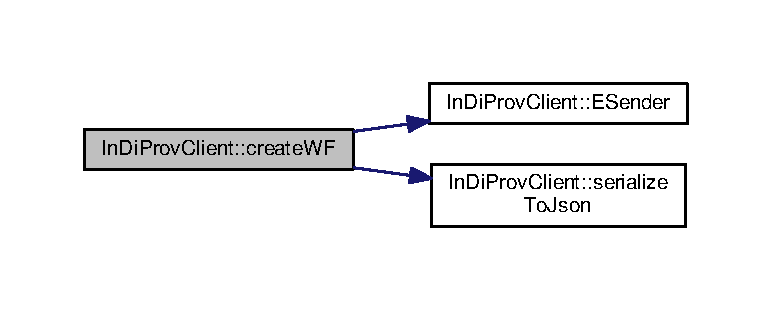
\includegraphics[width=350pt]{class_in_di_prov_client_aa8d9cbc951a6fd184e5156c3da84bc14_cgraph}
\end{center}
\end{figure}


\hypertarget{class_in_di_prov_client_ae99802bda1135179aa50a4413ef3c4e6}{\index{In\-Di\-Prov\-Client@{In\-Di\-Prov\-Client}!de\-Serialize\-Activities@{de\-Serialize\-Activities}}
\index{de\-Serialize\-Activities@{de\-Serialize\-Activities}!InDiProvClient@{In\-Di\-Prov\-Client}}
\subsubsection[{de\-Serialize\-Activities}]{\setlength{\rightskip}{0pt plus 5cm}vector$<$ {\bf Prov\-Utils\-::\-Activity} $>$ In\-Di\-Prov\-Client\-::de\-Serialize\-Activities (
\begin{DoxyParamCaption}
\item[{char $\ast$}]{activities\-Str}
\end{DoxyParamCaption}
)}}\label{class_in_di_prov_client_ae99802bda1135179aa50a4413ef3c4e6}


Exchange J\-S\-O\-N based Activities to vector$<$\-Prov\-Utils\-::\-Activity$>$ 

\hypertarget{class_in_di_prov_client_af3dd5119f070e70782d5d8cbeb15b3c4}{\index{In\-Di\-Prov\-Client@{In\-Di\-Prov\-Client}!de\-Serialize\-Agents@{de\-Serialize\-Agents}}
\index{de\-Serialize\-Agents@{de\-Serialize\-Agents}!InDiProvClient@{In\-Di\-Prov\-Client}}
\subsubsection[{de\-Serialize\-Agents}]{\setlength{\rightskip}{0pt plus 5cm}vector$<$ {\bf Prov\-Utils\-::\-Agent} $>$ In\-Di\-Prov\-Client\-::de\-Serialize\-Agents (
\begin{DoxyParamCaption}
\item[{char $\ast$}]{agents\-Str}
\end{DoxyParamCaption}
)}}\label{class_in_di_prov_client_af3dd5119f070e70782d5d8cbeb15b3c4}


Exchange J\-S\-O\-N based Agents to vector$<$\-Prov\-Utils\-::\-Agent$>$ 

\hypertarget{class_in_di_prov_client_af2de8cfed71d1340578e21794a32f1a1}{\index{In\-Di\-Prov\-Client@{In\-Di\-Prov\-Client}!de\-Serialize\-Entities@{de\-Serialize\-Entities}}
\index{de\-Serialize\-Entities@{de\-Serialize\-Entities}!InDiProvClient@{In\-Di\-Prov\-Client}}
\subsubsection[{de\-Serialize\-Entities}]{\setlength{\rightskip}{0pt plus 5cm}vector$<$ {\bf Prov\-Utils\-::\-Entity} $>$ In\-Di\-Prov\-Client\-::de\-Serialize\-Entities (
\begin{DoxyParamCaption}
\item[{char $\ast$}]{entities\-Str}
\end{DoxyParamCaption}
)}}\label{class_in_di_prov_client_af2de8cfed71d1340578e21794a32f1a1}


Exchange J\-S\-O\-N based Entities to vector$<$\-Prov\-Utils\-::\-Entity$>$ 

\hypertarget{class_in_di_prov_client_a6978eb897e437df621830f4859a79368}{\index{In\-Di\-Prov\-Client@{In\-Di\-Prov\-Client}!de\-Serialize\-Useds@{de\-Serialize\-Useds}}
\index{de\-Serialize\-Useds@{de\-Serialize\-Useds}!InDiProvClient@{In\-Di\-Prov\-Client}}
\subsubsection[{de\-Serialize\-Useds}]{\setlength{\rightskip}{0pt plus 5cm}vector$<$ {\bf Prov\-Utils\-::\-Used} $>$ In\-Di\-Prov\-Client\-::de\-Serialize\-Useds (
\begin{DoxyParamCaption}
\item[{char $\ast$}]{useds\-Str}
\end{DoxyParamCaption}
)}}\label{class_in_di_prov_client_a6978eb897e437df621830f4859a79368}


Exchange J\-S\-O\-N based Usages to vector$<$\-Prov\-Utils\-::\-Used$>$ 

\hypertarget{class_in_di_prov_client_a30ac2a5d87785c8bf7929d508bccf191}{\index{In\-Di\-Prov\-Client@{In\-Di\-Prov\-Client}!de\-Serialize\-Was\-Associated\-Withs@{de\-Serialize\-Was\-Associated\-Withs}}
\index{de\-Serialize\-Was\-Associated\-Withs@{de\-Serialize\-Was\-Associated\-Withs}!InDiProvClient@{In\-Di\-Prov\-Client}}
\subsubsection[{de\-Serialize\-Was\-Associated\-Withs}]{\setlength{\rightskip}{0pt plus 5cm}vector$<$ {\bf Prov\-Utils\-::\-Was\-Associated\-With} $>$ In\-Di\-Prov\-Client\-::de\-Serialize\-Was\-Associated\-Withs (
\begin{DoxyParamCaption}
\item[{char $\ast$}]{was\-Associated\-Withs\-Str}
\end{DoxyParamCaption}
)}}\label{class_in_di_prov_client_a30ac2a5d87785c8bf7929d508bccf191}


Exchange J\-S\-O\-N based Associations to vector$<$\-Prov\-Utils\-::\-Was\-Associated\-With$>$ 

\hypertarget{class_in_di_prov_client_a752ed9ff959b75d702f72346111d1676}{\index{In\-Di\-Prov\-Client@{In\-Di\-Prov\-Client}!de\-Serialize\-Was\-Attributed\-Tos@{de\-Serialize\-Was\-Attributed\-Tos}}
\index{de\-Serialize\-Was\-Attributed\-Tos@{de\-Serialize\-Was\-Attributed\-Tos}!InDiProvClient@{In\-Di\-Prov\-Client}}
\subsubsection[{de\-Serialize\-Was\-Attributed\-Tos}]{\setlength{\rightskip}{0pt plus 5cm}vector$<$ {\bf Prov\-Utils\-::\-Was\-Attributed\-To} $>$ In\-Di\-Prov\-Client\-::de\-Serialize\-Was\-Attributed\-Tos (
\begin{DoxyParamCaption}
\item[{char $\ast$}]{was\-Attributed\-To\-Str}
\end{DoxyParamCaption}
)}}\label{class_in_di_prov_client_a752ed9ff959b75d702f72346111d1676}


Exchange J\-S\-O\-N based Attributions to vector$<$\-Prov\-Utils\-::\-Was\-Attributed\-To$>$ 

\hypertarget{class_in_di_prov_client_ab68be507c04d2e4c27565489f045ac48}{\index{In\-Di\-Prov\-Client@{In\-Di\-Prov\-Client}!de\-Serialize\-Was\-Derived\-Froms@{de\-Serialize\-Was\-Derived\-Froms}}
\index{de\-Serialize\-Was\-Derived\-Froms@{de\-Serialize\-Was\-Derived\-Froms}!InDiProvClient@{In\-Di\-Prov\-Client}}
\subsubsection[{de\-Serialize\-Was\-Derived\-Froms}]{\setlength{\rightskip}{0pt plus 5cm}vector$<$ {\bf Prov\-Utils\-::\-Was\-Derived\-From} $>$ In\-Di\-Prov\-Client\-::de\-Serialize\-Was\-Derived\-Froms (
\begin{DoxyParamCaption}
\item[{char $\ast$}]{was\-Derived\-Froms\-Str}
\end{DoxyParamCaption}
)}}\label{class_in_di_prov_client_ab68be507c04d2e4c27565489f045ac48}


Exchange J\-S\-O\-N based Drivations to vector$<$\-Prov\-Utils\-::\-Was\-Derived\-From$>$ 

\hypertarget{class_in_di_prov_client_a5393f865d37acd18ef1af4e587eece29}{\index{In\-Di\-Prov\-Client@{In\-Di\-Prov\-Client}!de\-Serialize\-Was\-Ended\-Bys@{de\-Serialize\-Was\-Ended\-Bys}}
\index{de\-Serialize\-Was\-Ended\-Bys@{de\-Serialize\-Was\-Ended\-Bys}!InDiProvClient@{In\-Di\-Prov\-Client}}
\subsubsection[{de\-Serialize\-Was\-Ended\-Bys}]{\setlength{\rightskip}{0pt plus 5cm}vector$<$ {\bf Prov\-Utils\-::\-Was\-Ended\-By} $>$ In\-Di\-Prov\-Client\-::de\-Serialize\-Was\-Ended\-Bys (
\begin{DoxyParamCaption}
\item[{char $\ast$}]{Was\-Ended\-Bys\-Str}
\end{DoxyParamCaption}
)}}\label{class_in_di_prov_client_a5393f865d37acd18ef1af4e587eece29}


Exchange J\-S\-O\-N based Ends to vector$<$\-Prov\-Utils\-::\-Was\-Ended\-By$>$ 

\hypertarget{class_in_di_prov_client_afead00512a6bf04b3d134a3de1ab3909}{\index{In\-Di\-Prov\-Client@{In\-Di\-Prov\-Client}!de\-Serialize\-Was\-Generated\-Bys@{de\-Serialize\-Was\-Generated\-Bys}}
\index{de\-Serialize\-Was\-Generated\-Bys@{de\-Serialize\-Was\-Generated\-Bys}!InDiProvClient@{In\-Di\-Prov\-Client}}
\subsubsection[{de\-Serialize\-Was\-Generated\-Bys}]{\setlength{\rightskip}{0pt plus 5cm}vector$<$ {\bf Prov\-Utils\-::\-Was\-Generated\-By} $>$ In\-Di\-Prov\-Client\-::de\-Serialize\-Was\-Generated\-Bys (
\begin{DoxyParamCaption}
\item[{char $\ast$}]{was\-Generated\-Bys\-Str}
\end{DoxyParamCaption}
)}}\label{class_in_di_prov_client_afead00512a6bf04b3d134a3de1ab3909}


Exchange J\-S\-O\-N based Generations to vector$<$\-Prov\-Utils\-::\-Was\-Generated\-By$>$ 

\hypertarget{class_in_di_prov_client_a9c131081cbb7f6494d6d307d12559ddf}{\index{In\-Di\-Prov\-Client@{In\-Di\-Prov\-Client}!de\-Serialize\-Was\-Informed\-Bys@{de\-Serialize\-Was\-Informed\-Bys}}
\index{de\-Serialize\-Was\-Informed\-Bys@{de\-Serialize\-Was\-Informed\-Bys}!InDiProvClient@{In\-Di\-Prov\-Client}}
\subsubsection[{de\-Serialize\-Was\-Informed\-Bys}]{\setlength{\rightskip}{0pt plus 5cm}vector$<$ {\bf Prov\-Utils\-::\-Was\-Informed\-By} $>$ In\-Di\-Prov\-Client\-::de\-Serialize\-Was\-Informed\-Bys (
\begin{DoxyParamCaption}
\item[{char $\ast$}]{was\-Informed\-By\-Str}
\end{DoxyParamCaption}
)}}\label{class_in_di_prov_client_a9c131081cbb7f6494d6d307d12559ddf}


Exchange J\-S\-O\-N based Communications to vector$<$\-Prov\-Utils\-::\-Was\-Informed\-By$>$ 

\hypertarget{class_in_di_prov_client_a96f90e39262f2b956d05096231aa5801}{\index{In\-Di\-Prov\-Client@{In\-Di\-Prov\-Client}!de\-Serialize\-Was\-Started\-Bys@{de\-Serialize\-Was\-Started\-Bys}}
\index{de\-Serialize\-Was\-Started\-Bys@{de\-Serialize\-Was\-Started\-Bys}!InDiProvClient@{In\-Di\-Prov\-Client}}
\subsubsection[{de\-Serialize\-Was\-Started\-Bys}]{\setlength{\rightskip}{0pt plus 5cm}vector$<$ {\bf Prov\-Utils\-::\-Was\-Started\-By} $>$ In\-Di\-Prov\-Client\-::de\-Serialize\-Was\-Started\-Bys (
\begin{DoxyParamCaption}
\item[{char $\ast$}]{was\-Started\-Bys\-Str}
\end{DoxyParamCaption}
)}}\label{class_in_di_prov_client_a96f90e39262f2b956d05096231aa5801}


Exchange J\-S\-O\-N based Starts to vector$<$\-Prov\-Utils\-::\-Was\-Started\-By$>$ 

\hypertarget{class_in_di_prov_client_aa25fc27aead871d3a8103e27997cb2c6}{\index{In\-Di\-Prov\-Client@{In\-Di\-Prov\-Client}!E\-Sender@{E\-Sender}}
\index{E\-Sender@{E\-Sender}!InDiProvClient@{In\-Di\-Prov\-Client}}
\subsubsection[{E\-Sender}]{\setlength{\rightskip}{0pt plus 5cm}string In\-Di\-Prov\-Client\-::\-E\-Sender (
\begin{DoxyParamCaption}
\item[{string}]{msgstr}
\end{DoxyParamCaption}
)}}\label{class_in_di_prov_client_aa25fc27aead871d3a8103e27997cb2c6}


Send the J\-S\-O\-N based command to the defined server. 



Here is the caller graph for this function\-:
\nopagebreak
\begin{figure}[H]
\begin{center}
\leavevmode
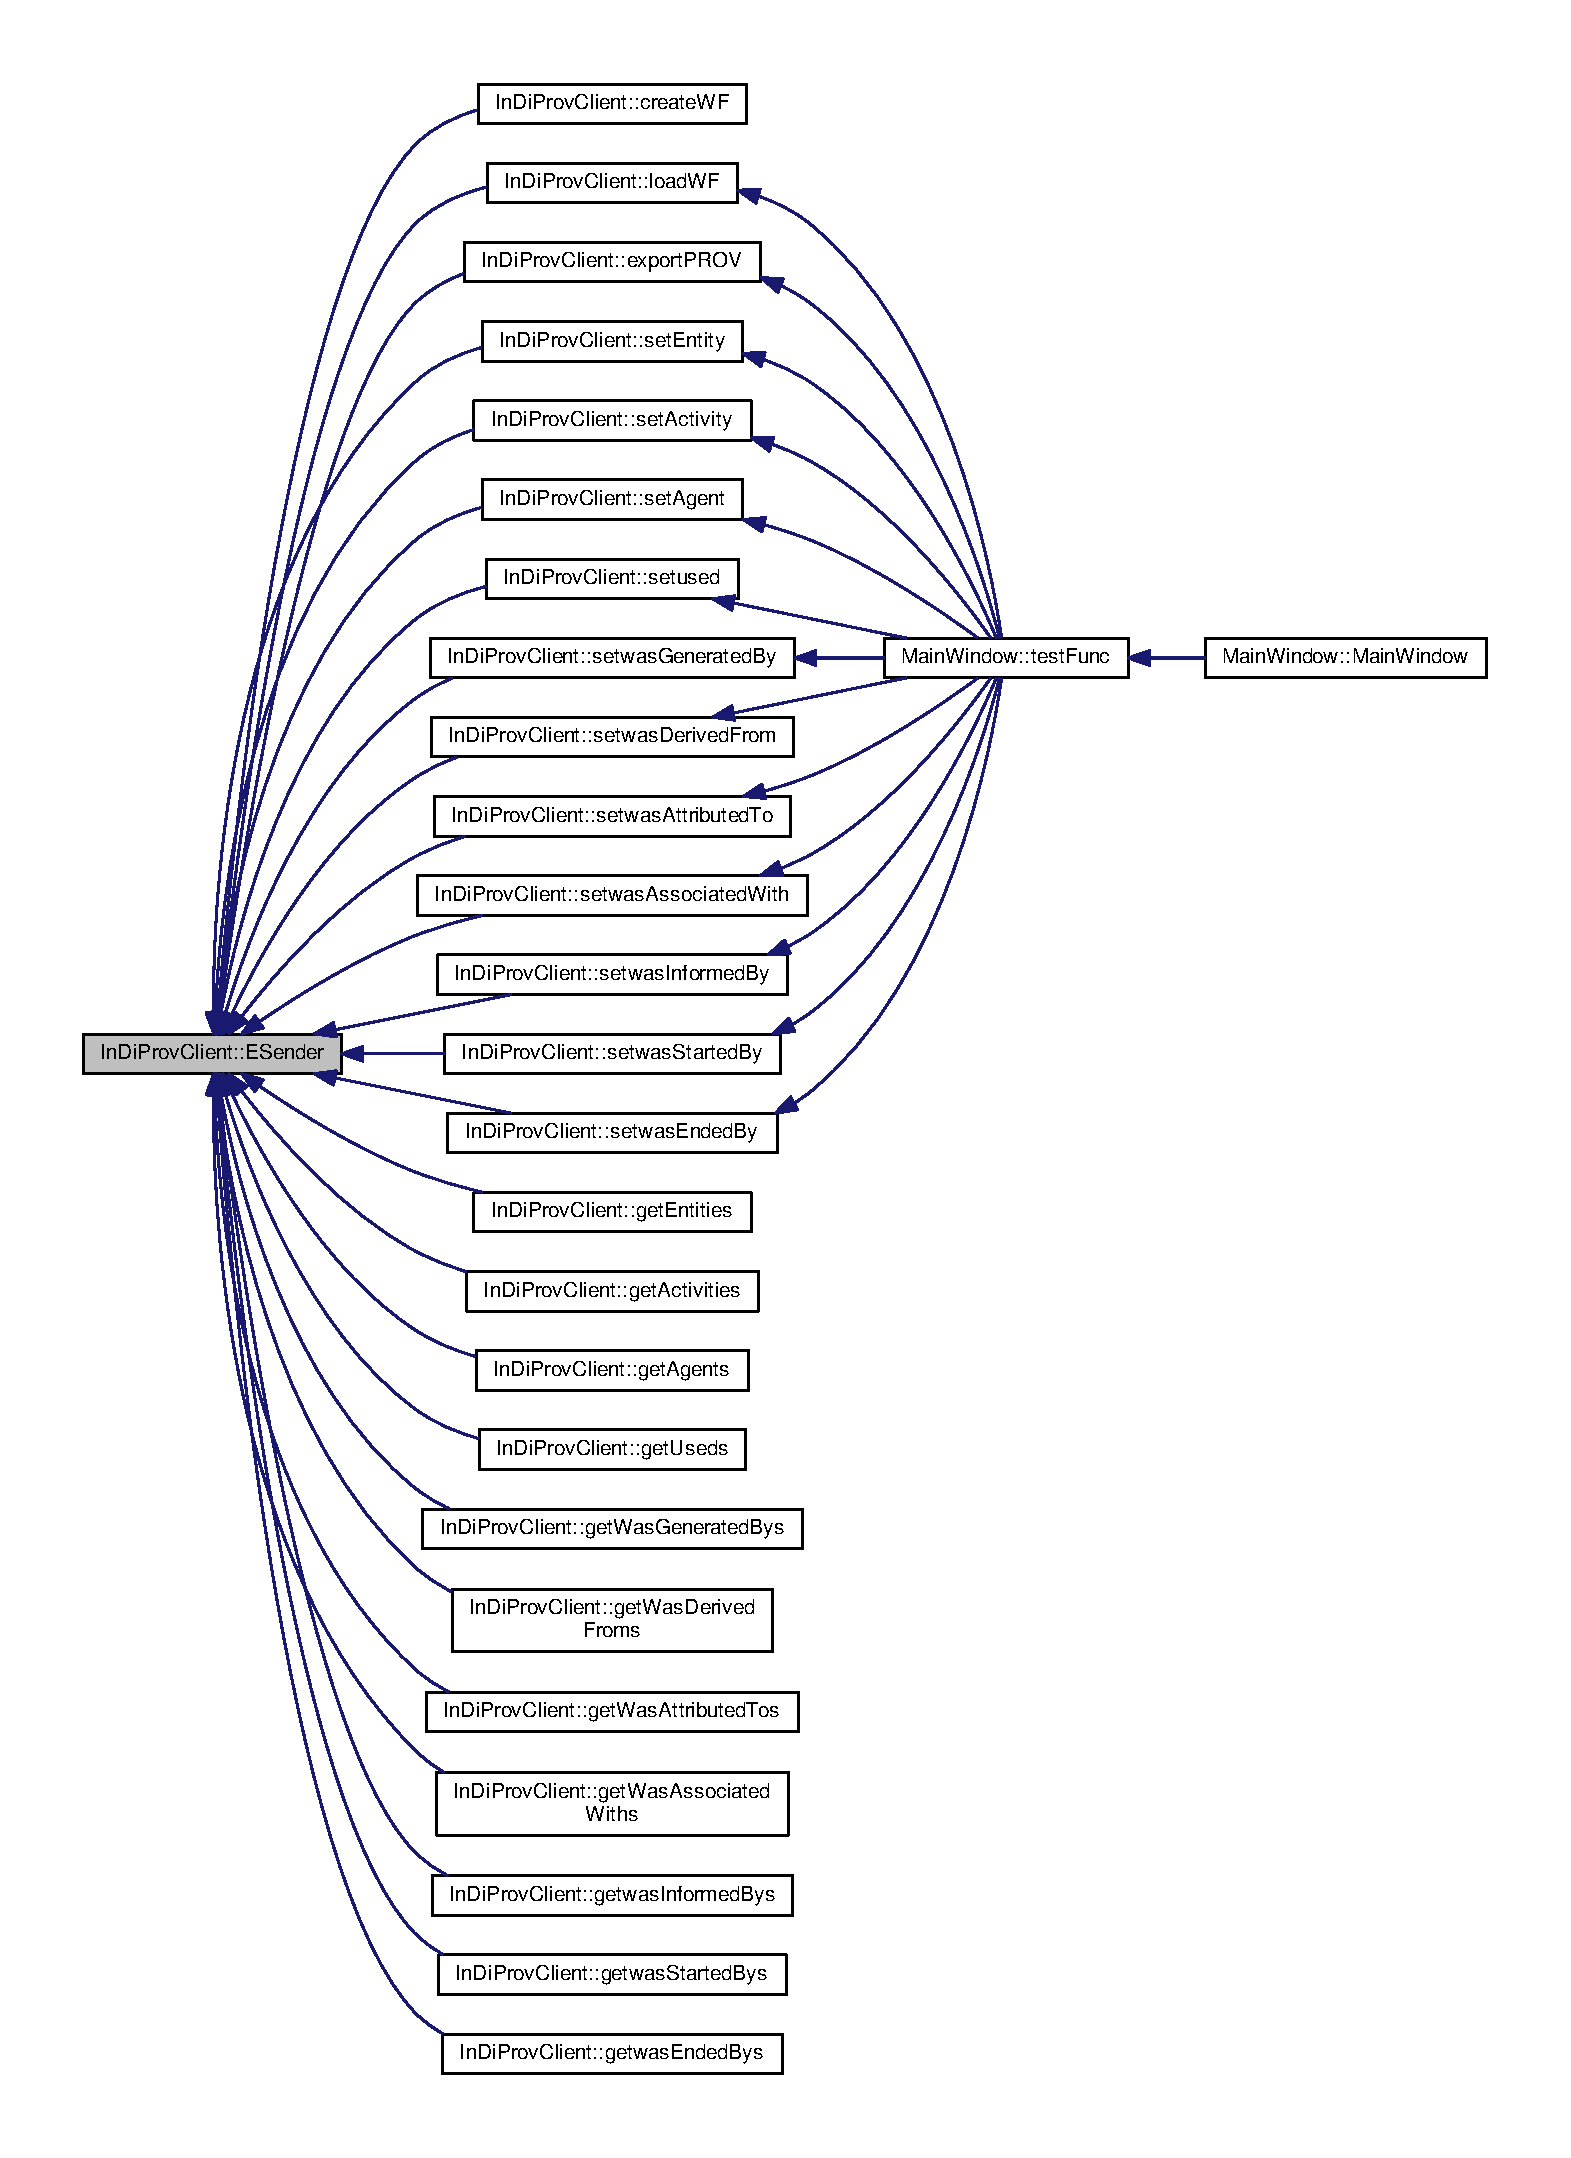
\includegraphics[width=350pt]{class_in_di_prov_client_aa25fc27aead871d3a8103e27997cb2c6_icgraph}
\end{center}
\end{figure}


\hypertarget{class_in_di_prov_client_a18211425d8d357513a16ff8314727470}{\index{In\-Di\-Prov\-Client@{In\-Di\-Prov\-Client}!export\-P\-R\-O\-V@{export\-P\-R\-O\-V}}
\index{export\-P\-R\-O\-V@{export\-P\-R\-O\-V}!InDiProvClient@{In\-Di\-Prov\-Client}}
\subsubsection[{export\-P\-R\-O\-V}]{\setlength{\rightskip}{0pt plus 5cm}int In\-Di\-Prov\-Client\-::export\-P\-R\-O\-V (
\begin{DoxyParamCaption}
{}
\end{DoxyParamCaption}
)}}\label{class_in_di_prov_client_a18211425d8d357513a16ff8314727470}


Export the current provenance information into xml format. 



Here is the call graph for this function\-:
\nopagebreak
\begin{figure}[H]
\begin{center}
\leavevmode
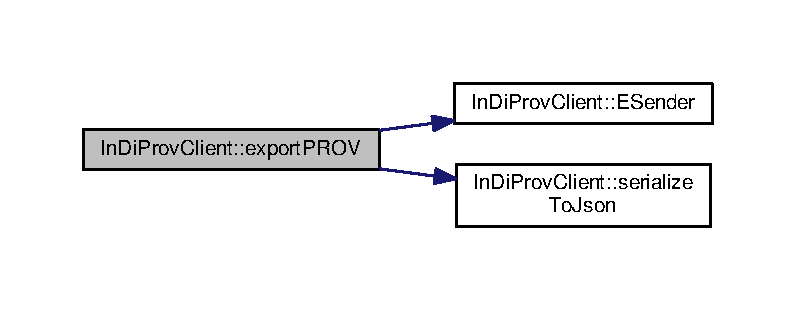
\includegraphics[width=350pt]{class_in_di_prov_client_a18211425d8d357513a16ff8314727470_cgraph}
\end{center}
\end{figure}




Here is the caller graph for this function\-:
\nopagebreak
\begin{figure}[H]
\begin{center}
\leavevmode
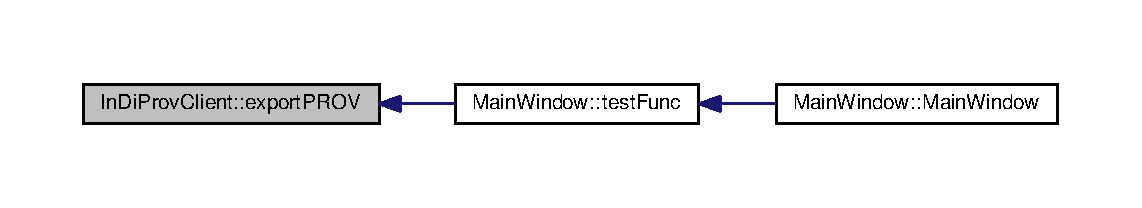
\includegraphics[width=350pt]{class_in_di_prov_client_a18211425d8d357513a16ff8314727470_icgraph}
\end{center}
\end{figure}


\hypertarget{class_in_di_prov_client_a07d2197c8cce39ba7dd33edbfd09af78}{\index{In\-Di\-Prov\-Client@{In\-Di\-Prov\-Client}!get\-Activities@{get\-Activities}}
\index{get\-Activities@{get\-Activities}!InDiProvClient@{In\-Di\-Prov\-Client}}
\subsubsection[{get\-Activities}]{\setlength{\rightskip}{0pt plus 5cm}string In\-Di\-Prov\-Client\-::get\-Activities (
\begin{DoxyParamCaption}
{}
\end{DoxyParamCaption}
)}}\label{class_in_di_prov_client_a07d2197c8cce39ba7dd33edbfd09af78}


Retrieving all Activities from the loaded workflow in J\-S\-O\-N based. 



Here is the call graph for this function\-:
\nopagebreak
\begin{figure}[H]
\begin{center}
\leavevmode
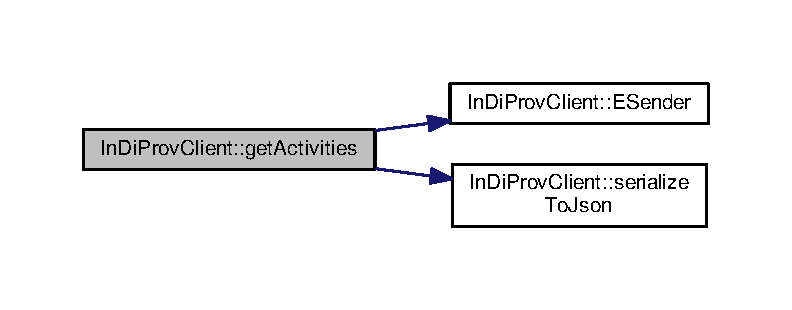
\includegraphics[width=350pt]{class_in_di_prov_client_a07d2197c8cce39ba7dd33edbfd09af78_cgraph}
\end{center}
\end{figure}


\hypertarget{class_in_di_prov_client_ab4b6f77ddb41281dd8714c7742faafbc}{\index{In\-Di\-Prov\-Client@{In\-Di\-Prov\-Client}!get\-Agents@{get\-Agents}}
\index{get\-Agents@{get\-Agents}!InDiProvClient@{In\-Di\-Prov\-Client}}
\subsubsection[{get\-Agents}]{\setlength{\rightskip}{0pt plus 5cm}string In\-Di\-Prov\-Client\-::get\-Agents (
\begin{DoxyParamCaption}
{}
\end{DoxyParamCaption}
)}}\label{class_in_di_prov_client_ab4b6f77ddb41281dd8714c7742faafbc}


Retrieving all Agents from the loaded workflow in J\-S\-O\-N based. 



Here is the call graph for this function\-:
\nopagebreak
\begin{figure}[H]
\begin{center}
\leavevmode
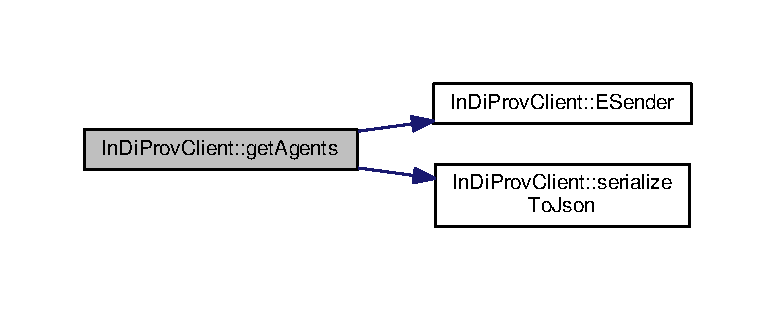
\includegraphics[width=350pt]{class_in_di_prov_client_ab4b6f77ddb41281dd8714c7742faafbc_cgraph}
\end{center}
\end{figure}


\hypertarget{class_in_di_prov_client_a6844299f790bb3e1f460b64fca2a2585}{\index{In\-Di\-Prov\-Client@{In\-Di\-Prov\-Client}!get\-Current\-Time@{get\-Current\-Time}}
\index{get\-Current\-Time@{get\-Current\-Time}!InDiProvClient@{In\-Di\-Prov\-Client}}
\subsubsection[{get\-Current\-Time}]{\setlength{\rightskip}{0pt plus 5cm}string In\-Di\-Prov\-Client\-::get\-Current\-Time (
\begin{DoxyParamCaption}
{}
\end{DoxyParamCaption}
)}}\label{class_in_di_prov_client_a6844299f790bb3e1f460b64fca2a2585}
Returns the current time of the client in string format. Important\-: Just use this function as time string argument. 

Here is the caller graph for this function\-:
\nopagebreak
\begin{figure}[H]
\begin{center}
\leavevmode
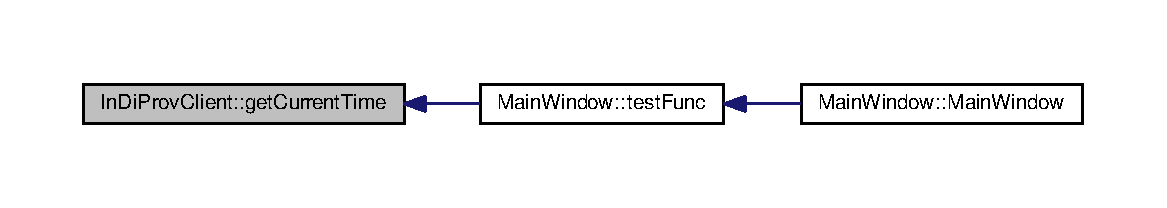
\includegraphics[width=350pt]{class_in_di_prov_client_a6844299f790bb3e1f460b64fca2a2585_icgraph}
\end{center}
\end{figure}


\hypertarget{class_in_di_prov_client_aa2e07af7b32a73889ef3332f04bbcf1a}{\index{In\-Di\-Prov\-Client@{In\-Di\-Prov\-Client}!get\-Entities@{get\-Entities}}
\index{get\-Entities@{get\-Entities}!InDiProvClient@{In\-Di\-Prov\-Client}}
\subsubsection[{get\-Entities}]{\setlength{\rightskip}{0pt plus 5cm}string In\-Di\-Prov\-Client\-::get\-Entities (
\begin{DoxyParamCaption}
{}
\end{DoxyParamCaption}
)}}\label{class_in_di_prov_client_aa2e07af7b32a73889ef3332f04bbcf1a}


Retrieving all Entities from the loaded workflow in J\-S\-O\-N based. 



Here is the call graph for this function\-:
\nopagebreak
\begin{figure}[H]
\begin{center}
\leavevmode
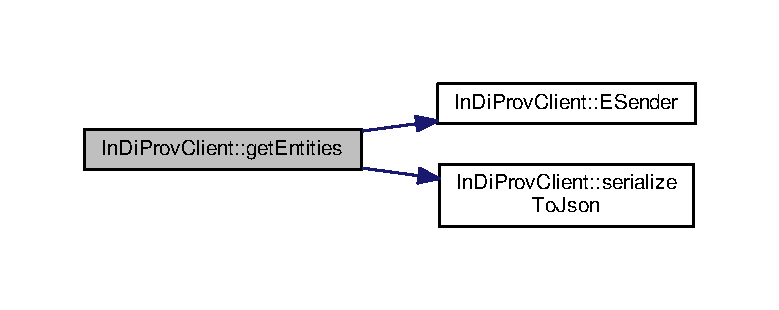
\includegraphics[width=350pt]{class_in_di_prov_client_aa2e07af7b32a73889ef3332f04bbcf1a_cgraph}
\end{center}
\end{figure}


\hypertarget{class_in_di_prov_client_a88514328d91e2c6946b343176fabf650}{\index{In\-Di\-Prov\-Client@{In\-Di\-Prov\-Client}!get\-Useds@{get\-Useds}}
\index{get\-Useds@{get\-Useds}!InDiProvClient@{In\-Di\-Prov\-Client}}
\subsubsection[{get\-Useds}]{\setlength{\rightskip}{0pt plus 5cm}string In\-Di\-Prov\-Client\-::get\-Useds (
\begin{DoxyParamCaption}
{}
\end{DoxyParamCaption}
)}}\label{class_in_di_prov_client_a88514328d91e2c6946b343176fabf650}


Retrieving all Usages from the loaded workflow in J\-S\-O\-N based. 



Here is the call graph for this function\-:
\nopagebreak
\begin{figure}[H]
\begin{center}
\leavevmode
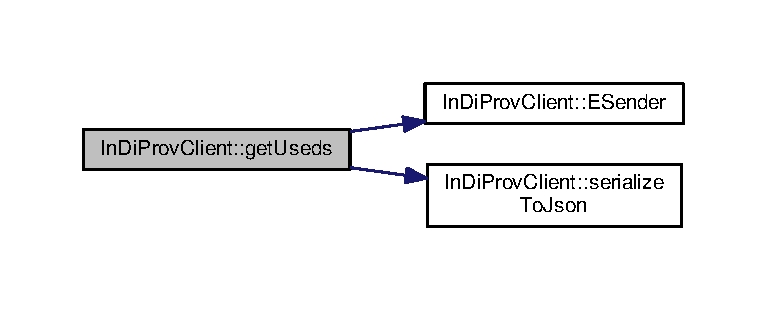
\includegraphics[width=350pt]{class_in_di_prov_client_a88514328d91e2c6946b343176fabf650_cgraph}
\end{center}
\end{figure}


\hypertarget{class_in_di_prov_client_af0c7484225b5415c89b10f73f61ad3d1}{\index{In\-Di\-Prov\-Client@{In\-Di\-Prov\-Client}!get\-Was\-Associated\-Withs@{get\-Was\-Associated\-Withs}}
\index{get\-Was\-Associated\-Withs@{get\-Was\-Associated\-Withs}!InDiProvClient@{In\-Di\-Prov\-Client}}
\subsubsection[{get\-Was\-Associated\-Withs}]{\setlength{\rightskip}{0pt plus 5cm}string In\-Di\-Prov\-Client\-::get\-Was\-Associated\-Withs (
\begin{DoxyParamCaption}
{}
\end{DoxyParamCaption}
)}}\label{class_in_di_prov_client_af0c7484225b5415c89b10f73f61ad3d1}


Retrieving all Associations from the loaded workflow in J\-S\-O\-N based. 



Here is the call graph for this function\-:
\nopagebreak
\begin{figure}[H]
\begin{center}
\leavevmode
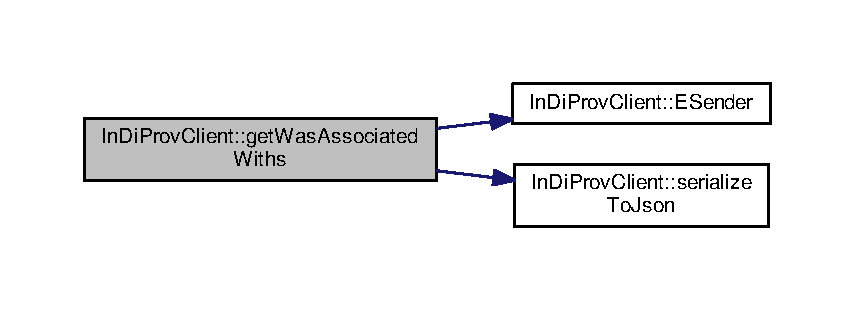
\includegraphics[width=350pt]{class_in_di_prov_client_af0c7484225b5415c89b10f73f61ad3d1_cgraph}
\end{center}
\end{figure}


\hypertarget{class_in_di_prov_client_a73cf344a968785eb407488c423e00cf2}{\index{In\-Di\-Prov\-Client@{In\-Di\-Prov\-Client}!get\-Was\-Attributed\-Tos@{get\-Was\-Attributed\-Tos}}
\index{get\-Was\-Attributed\-Tos@{get\-Was\-Attributed\-Tos}!InDiProvClient@{In\-Di\-Prov\-Client}}
\subsubsection[{get\-Was\-Attributed\-Tos}]{\setlength{\rightskip}{0pt plus 5cm}string In\-Di\-Prov\-Client\-::get\-Was\-Attributed\-Tos (
\begin{DoxyParamCaption}
{}
\end{DoxyParamCaption}
)}}\label{class_in_di_prov_client_a73cf344a968785eb407488c423e00cf2}


Retrieving all Attributions from the loaded workflow in J\-S\-O\-N based. 



Here is the call graph for this function\-:
\nopagebreak
\begin{figure}[H]
\begin{center}
\leavevmode
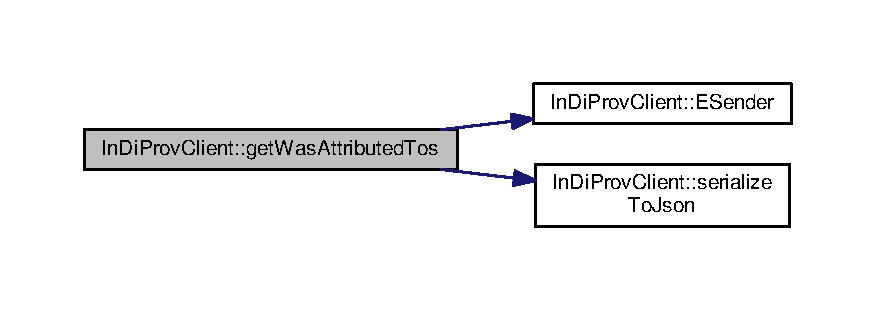
\includegraphics[width=350pt]{class_in_di_prov_client_a73cf344a968785eb407488c423e00cf2_cgraph}
\end{center}
\end{figure}


\hypertarget{class_in_di_prov_client_adffc2e33efbc970dbb2f8bb7c5332744}{\index{In\-Di\-Prov\-Client@{In\-Di\-Prov\-Client}!get\-Was\-Derived\-Froms@{get\-Was\-Derived\-Froms}}
\index{get\-Was\-Derived\-Froms@{get\-Was\-Derived\-Froms}!InDiProvClient@{In\-Di\-Prov\-Client}}
\subsubsection[{get\-Was\-Derived\-Froms}]{\setlength{\rightskip}{0pt plus 5cm}string In\-Di\-Prov\-Client\-::get\-Was\-Derived\-Froms (
\begin{DoxyParamCaption}
{}
\end{DoxyParamCaption}
)}}\label{class_in_di_prov_client_adffc2e33efbc970dbb2f8bb7c5332744}


Retrieving all Derivations from the loaded workflow in J\-S\-O\-N based. 



Here is the call graph for this function\-:
\nopagebreak
\begin{figure}[H]
\begin{center}
\leavevmode
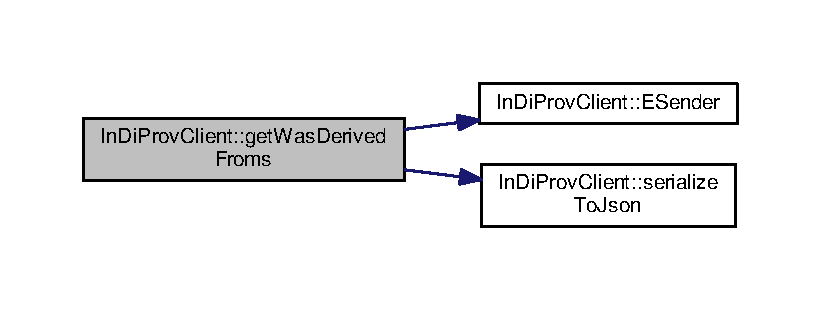
\includegraphics[width=350pt]{class_in_di_prov_client_adffc2e33efbc970dbb2f8bb7c5332744_cgraph}
\end{center}
\end{figure}


\hypertarget{class_in_di_prov_client_ab7946e8a31014d95bf03250b6b466bb1}{\index{In\-Di\-Prov\-Client@{In\-Di\-Prov\-Client}!getwas\-Ended\-Bys@{getwas\-Ended\-Bys}}
\index{getwas\-Ended\-Bys@{getwas\-Ended\-Bys}!InDiProvClient@{In\-Di\-Prov\-Client}}
\subsubsection[{getwas\-Ended\-Bys}]{\setlength{\rightskip}{0pt plus 5cm}string In\-Di\-Prov\-Client\-::getwas\-Ended\-Bys (
\begin{DoxyParamCaption}
{}
\end{DoxyParamCaption}
)}}\label{class_in_di_prov_client_ab7946e8a31014d95bf03250b6b466bb1}


Retrieving all Ends from the loaded workflow in J\-S\-O\-N based. 



Here is the call graph for this function\-:
\nopagebreak
\begin{figure}[H]
\begin{center}
\leavevmode
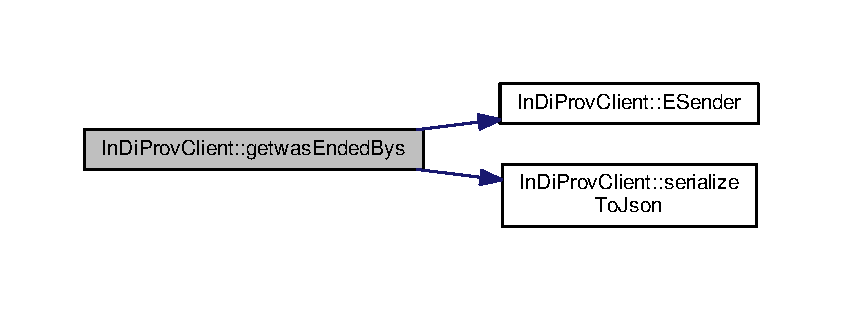
\includegraphics[width=350pt]{class_in_di_prov_client_ab7946e8a31014d95bf03250b6b466bb1_cgraph}
\end{center}
\end{figure}


\hypertarget{class_in_di_prov_client_abe2dc19daa8dfa5b04fb3ac623e47bc0}{\index{In\-Di\-Prov\-Client@{In\-Di\-Prov\-Client}!get\-Was\-Generated\-Bys@{get\-Was\-Generated\-Bys}}
\index{get\-Was\-Generated\-Bys@{get\-Was\-Generated\-Bys}!InDiProvClient@{In\-Di\-Prov\-Client}}
\subsubsection[{get\-Was\-Generated\-Bys}]{\setlength{\rightskip}{0pt plus 5cm}string In\-Di\-Prov\-Client\-::get\-Was\-Generated\-Bys (
\begin{DoxyParamCaption}
{}
\end{DoxyParamCaption}
)}}\label{class_in_di_prov_client_abe2dc19daa8dfa5b04fb3ac623e47bc0}


Retrieving all Generations from the loaded workflow in J\-S\-O\-N based. 



Here is the call graph for this function\-:
\nopagebreak
\begin{figure}[H]
\begin{center}
\leavevmode
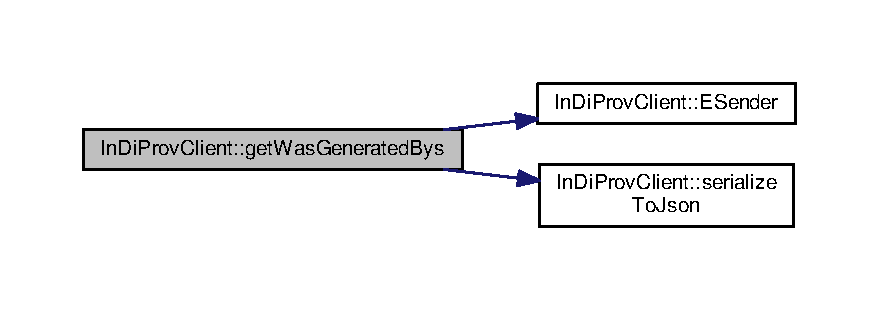
\includegraphics[width=350pt]{class_in_di_prov_client_abe2dc19daa8dfa5b04fb3ac623e47bc0_cgraph}
\end{center}
\end{figure}


\hypertarget{class_in_di_prov_client_a1ca1cc7ed3c7f08451ae78a2af50b223}{\index{In\-Di\-Prov\-Client@{In\-Di\-Prov\-Client}!getwas\-Informed\-Bys@{getwas\-Informed\-Bys}}
\index{getwas\-Informed\-Bys@{getwas\-Informed\-Bys}!InDiProvClient@{In\-Di\-Prov\-Client}}
\subsubsection[{getwas\-Informed\-Bys}]{\setlength{\rightskip}{0pt plus 5cm}string In\-Di\-Prov\-Client\-::getwas\-Informed\-Bys (
\begin{DoxyParamCaption}
{}
\end{DoxyParamCaption}
)}}\label{class_in_di_prov_client_a1ca1cc7ed3c7f08451ae78a2af50b223}


Retrieving all Communications from the loaded workflow in J\-S\-O\-N based. 



Here is the call graph for this function\-:
\nopagebreak
\begin{figure}[H]
\begin{center}
\leavevmode
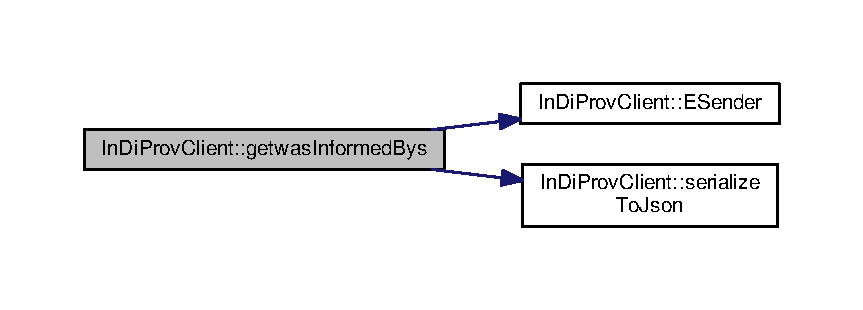
\includegraphics[width=350pt]{class_in_di_prov_client_a1ca1cc7ed3c7f08451ae78a2af50b223_cgraph}
\end{center}
\end{figure}


\hypertarget{class_in_di_prov_client_aef39fc253d97b3534b8772ece2d01735}{\index{In\-Di\-Prov\-Client@{In\-Di\-Prov\-Client}!getwas\-Started\-Bys@{getwas\-Started\-Bys}}
\index{getwas\-Started\-Bys@{getwas\-Started\-Bys}!InDiProvClient@{In\-Di\-Prov\-Client}}
\subsubsection[{getwas\-Started\-Bys}]{\setlength{\rightskip}{0pt plus 5cm}string In\-Di\-Prov\-Client\-::getwas\-Started\-Bys (
\begin{DoxyParamCaption}
{}
\end{DoxyParamCaption}
)}}\label{class_in_di_prov_client_aef39fc253d97b3534b8772ece2d01735}


Retrieving all Starts from the loaded workflow in J\-S\-O\-N based. 



Here is the call graph for this function\-:
\nopagebreak
\begin{figure}[H]
\begin{center}
\leavevmode
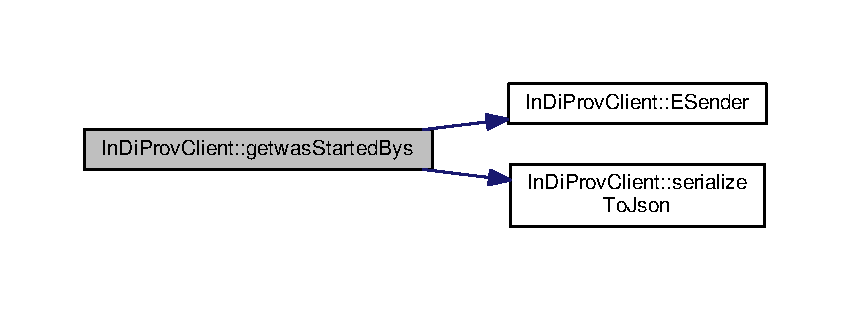
\includegraphics[width=350pt]{class_in_di_prov_client_aef39fc253d97b3534b8772ece2d01735_cgraph}
\end{center}
\end{figure}


\hypertarget{class_in_di_prov_client_ab4cd3159aff7a597b2a394a43b589003}{\index{In\-Di\-Prov\-Client@{In\-Di\-Prov\-Client}!get\-W\-F\-I\-D@{get\-W\-F\-I\-D}}
\index{get\-W\-F\-I\-D@{get\-W\-F\-I\-D}!InDiProvClient@{In\-Di\-Prov\-Client}}
\subsubsection[{get\-W\-F\-I\-D}]{\setlength{\rightskip}{0pt plus 5cm}int In\-Di\-Prov\-Client\-::get\-W\-F\-I\-D (
\begin{DoxyParamCaption}
{}
\end{DoxyParamCaption}
)}}\label{class_in_di_prov_client_ab4cd3159aff7a597b2a394a43b589003}


Returns the current W\-F\-I\-D, -\/1 means no W\-F is selected. 

\hypertarget{class_in_di_prov_client_aa45bb40b1c500fbd4a7a9abd862e7f82}{\index{In\-Di\-Prov\-Client@{In\-Di\-Prov\-Client}!get\-W\-F\-Pass@{get\-W\-F\-Pass}}
\index{get\-W\-F\-Pass@{get\-W\-F\-Pass}!InDiProvClient@{In\-Di\-Prov\-Client}}
\subsubsection[{get\-W\-F\-Pass}]{\setlength{\rightskip}{0pt plus 5cm}string In\-Di\-Prov\-Client\-::get\-W\-F\-Pass (
\begin{DoxyParamCaption}
{}
\end{DoxyParamCaption}
)}}\label{class_in_di_prov_client_aa45bb40b1c500fbd4a7a9abd862e7f82}


Returns the current W\-F\-Pass (workflow passwords) 

\hypertarget{class_in_di_prov_client_ae4bca8e968f14753a1fd6e7b59b92f3c}{\index{In\-Di\-Prov\-Client@{In\-Di\-Prov\-Client}!json\-\_\-parse@{json\-\_\-parse}}
\index{json\-\_\-parse@{json\-\_\-parse}!InDiProvClient@{In\-Di\-Prov\-Client}}
\subsubsection[{json\-\_\-parse}]{\setlength{\rightskip}{0pt plus 5cm}void In\-Di\-Prov\-Client\-::json\-\_\-parse (
\begin{DoxyParamCaption}
\item[{json\-\_\-object $\ast$}]{jobj}
\end{DoxyParamCaption}
)}}\label{class_in_di_prov_client_ae4bca8e968f14753a1fd6e7b59b92f3c}
\hypertarget{class_in_di_prov_client_ae2e0dd71c6b83274706f1bb26742cabe}{\index{In\-Di\-Prov\-Client@{In\-Di\-Prov\-Client}!load\-W\-F@{load\-W\-F}}
\index{load\-W\-F@{load\-W\-F}!InDiProvClient@{In\-Di\-Prov\-Client}}
\subsubsection[{load\-W\-F}]{\setlength{\rightskip}{0pt plus 5cm}int In\-Di\-Prov\-Client\-::load\-W\-F (
\begin{DoxyParamCaption}
\item[{int}]{W\-Fid, }
\item[{string}]{password}
\end{DoxyParamCaption}
)}}\label{class_in_di_prov_client_ae2e0dd71c6b83274706f1bb26742cabe}
Loading workflow with corresponding id and password. Returns the the same id if the function is successful, else returns -\/1. Also the W\-F\-I\-D and W\-F\-Pass variables of the object will be updated if if the function is successful. 

Here is the call graph for this function\-:
\nopagebreak
\begin{figure}[H]
\begin{center}
\leavevmode
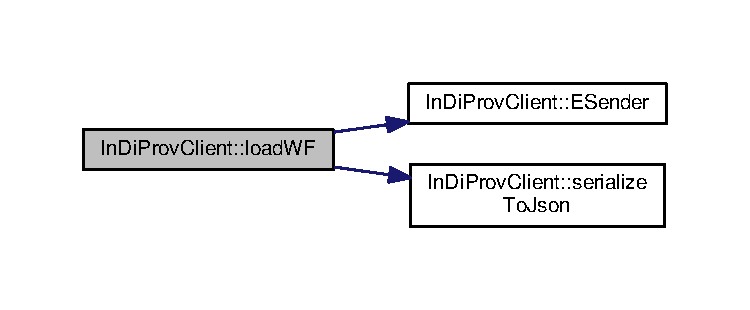
\includegraphics[width=350pt]{class_in_di_prov_client_ae2e0dd71c6b83274706f1bb26742cabe_cgraph}
\end{center}
\end{figure}




Here is the caller graph for this function\-:
\nopagebreak
\begin{figure}[H]
\begin{center}
\leavevmode
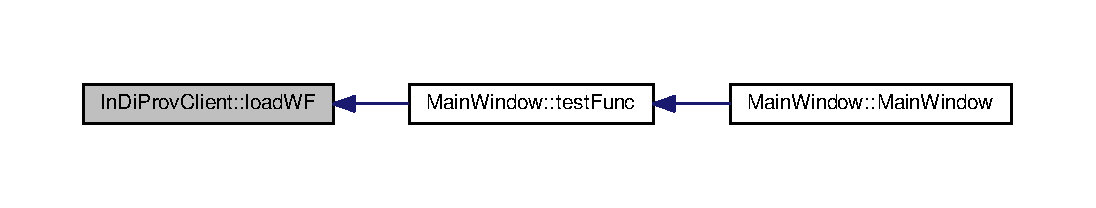
\includegraphics[width=350pt]{class_in_di_prov_client_ae2e0dd71c6b83274706f1bb26742cabe_icgraph}
\end{center}
\end{figure}


\hypertarget{class_in_di_prov_client_af7cb9082299c4dd099c176b55899dff0}{\index{In\-Di\-Prov\-Client@{In\-Di\-Prov\-Client}!serialize\-To\-Json@{serialize\-To\-Json}}
\index{serialize\-To\-Json@{serialize\-To\-Json}!InDiProvClient@{In\-Di\-Prov\-Client}}
\subsubsection[{serialize\-To\-Json}]{\setlength{\rightskip}{0pt plus 5cm}string In\-Di\-Prov\-Client\-::serialize\-To\-Json (
\begin{DoxyParamCaption}
\item[{vector$<$ string $>$}]{command\-Vec}
\end{DoxyParamCaption}
)}}\label{class_in_di_prov_client_af7cb9082299c4dd099c176b55899dff0}


Serialize command/function into J\-S\-O\-N based. 



Here is the caller graph for this function\-:
\nopagebreak
\begin{figure}[H]
\begin{center}
\leavevmode
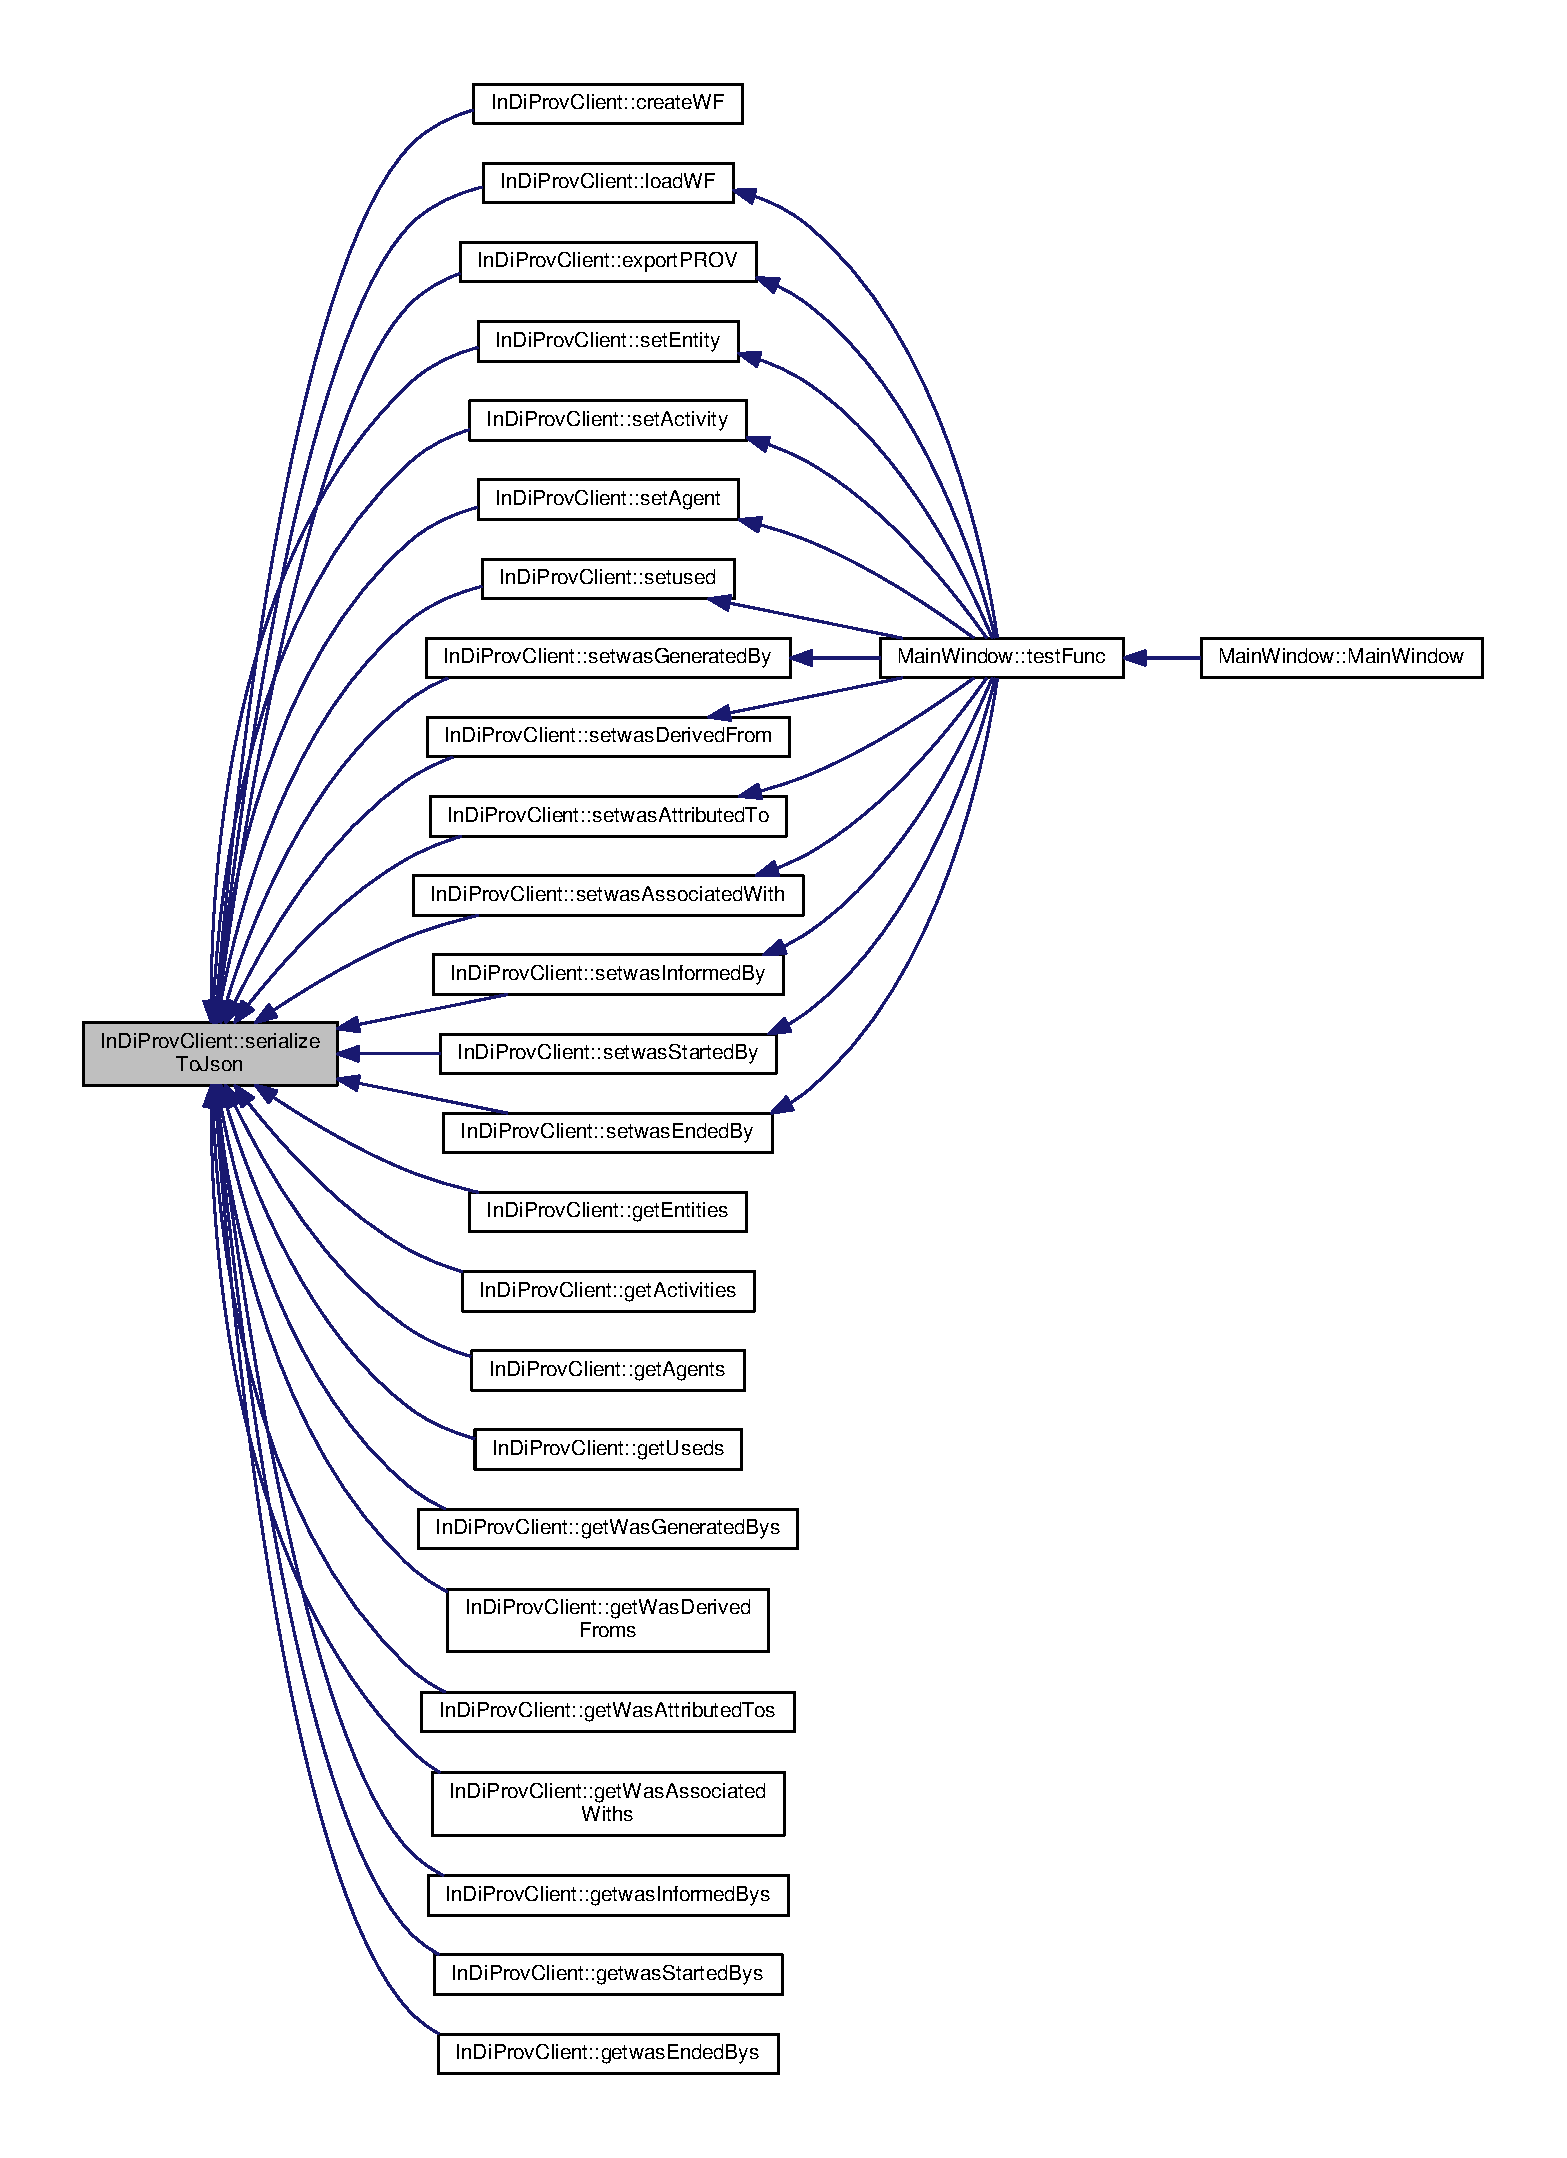
\includegraphics[width=350pt]{class_in_di_prov_client_af7cb9082299c4dd099c176b55899dff0_icgraph}
\end{center}
\end{figure}


\hypertarget{class_in_di_prov_client_a8a2e2aaf3f8b6a8e31f31af31603b681}{\index{In\-Di\-Prov\-Client@{In\-Di\-Prov\-Client}!set\-Activity@{set\-Activity}}
\index{set\-Activity@{set\-Activity}!InDiProvClient@{In\-Di\-Prov\-Client}}
\subsubsection[{set\-Activity}]{\setlength{\rightskip}{0pt plus 5cm}int In\-Di\-Prov\-Client\-::set\-Activity (
\begin{DoxyParamCaption}
\item[{string}]{start\-Time, }
\item[{string}]{end\-Time, }
\item[{string}]{label, }
\item[{string}]{location, }
\item[{string}]{type}
\end{DoxyParamCaption}
)}}\label{class_in_di_prov_client_a8a2e2aaf3f8b6a8e31f31af31603b681}


Creating new Activity returns the unique id of new Activity if the function is successful, else returns -\/1. 

An activity is something that occurs over a period of time and acts upon or with entities; it may include consuming, processing, transforming, modifying, relocating, using, or generating entities. Just as entities cover a broad range of notions, activities can cover a broad range of notions\-: information processing activities may for example move, copy, or duplicate digital entities; physical activities can include driving a car between two locations or printing a book.\par
 Example\-: An activity may be the publishing of a document on the Web, sending a twitter message, extracting metadata embedded in a file, driving a car from Boston to Cambridge, assembling a data set based on a set of measurements, performing a statistical analysis over a data set, sorting news items according to some criteria, running a S\-P\-A\-R\-Q\-L query over a triple store, or editing a file. 

Here is the call graph for this function\-:
\nopagebreak
\begin{figure}[H]
\begin{center}
\leavevmode
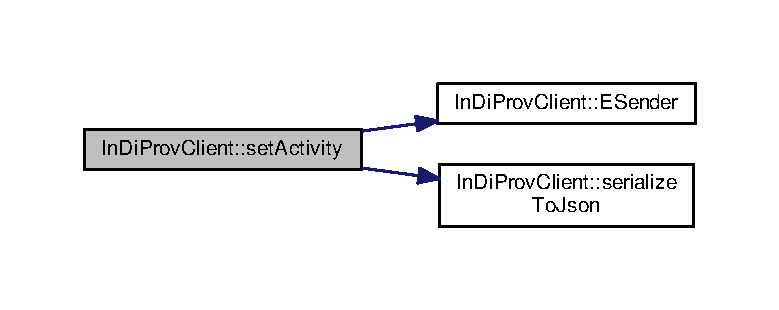
\includegraphics[width=350pt]{class_in_di_prov_client_a8a2e2aaf3f8b6a8e31f31af31603b681_cgraph}
\end{center}
\end{figure}




Here is the caller graph for this function\-:
\nopagebreak
\begin{figure}[H]
\begin{center}
\leavevmode
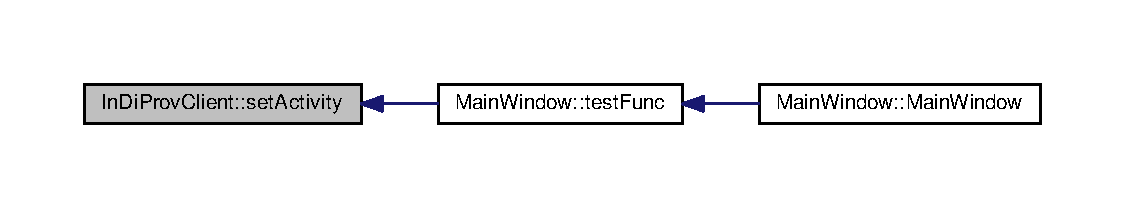
\includegraphics[width=350pt]{class_in_di_prov_client_a8a2e2aaf3f8b6a8e31f31af31603b681_icgraph}
\end{center}
\end{figure}


\hypertarget{class_in_di_prov_client_a75ad36497b77b81841cf8cf411aea244}{\index{In\-Di\-Prov\-Client@{In\-Di\-Prov\-Client}!set\-Agent@{set\-Agent}}
\index{set\-Agent@{set\-Agent}!InDiProvClient@{In\-Di\-Prov\-Client}}
\subsubsection[{set\-Agent}]{\setlength{\rightskip}{0pt plus 5cm}int In\-Di\-Prov\-Client\-::set\-Agent (
\begin{DoxyParamCaption}
\item[{string}]{label, }
\item[{string}]{location, }
\item[{string}]{type}
\end{DoxyParamCaption}
)}}\label{class_in_di_prov_client_a75ad36497b77b81841cf8cf411aea244}


Creating new Agent returns the unique id of new Agent if the function is successful, else returns -\/1. 

For many purposes, a key consideration for deciding whether something is reliable and/or trustworthy is knowing who or what was reponsible for its production. Data published by a respected independent organization may be considered more trustworthy than that from a lobby organization; a claim by a well-\/known scientist with an established track record may be more believed than a claim by a new student; a calculation performed by an established software library may be more reliable than by a one-\/off program. An agent is something that bears some form of responsibility for an activity taking place, for the existence of an entity, or for another agent's activity. An agent may be a particular type of entity or activity. This means that the model can be used to express provenance of the agents themselves.\par
 Example\-: Software for checking the use of grammar in a document may be defined as an agent of a document preparation activity; one can also describe its provenance, including for instance the vendor and the version history. A site selling books on the Web, the services involved in the processing of orders, and the companies hosting them are also agents. 

Here is the call graph for this function\-:
\nopagebreak
\begin{figure}[H]
\begin{center}
\leavevmode
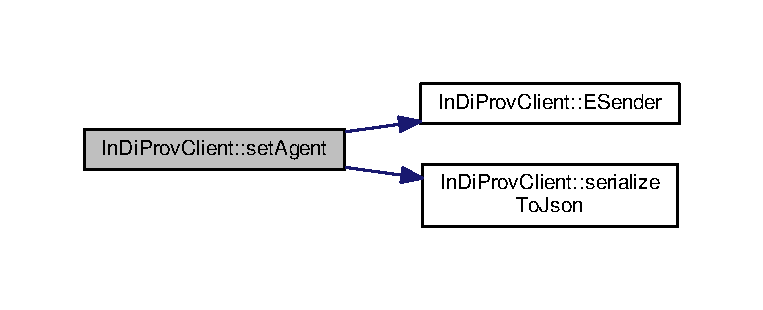
\includegraphics[width=350pt]{class_in_di_prov_client_a75ad36497b77b81841cf8cf411aea244_cgraph}
\end{center}
\end{figure}




Here is the caller graph for this function\-:
\nopagebreak
\begin{figure}[H]
\begin{center}
\leavevmode
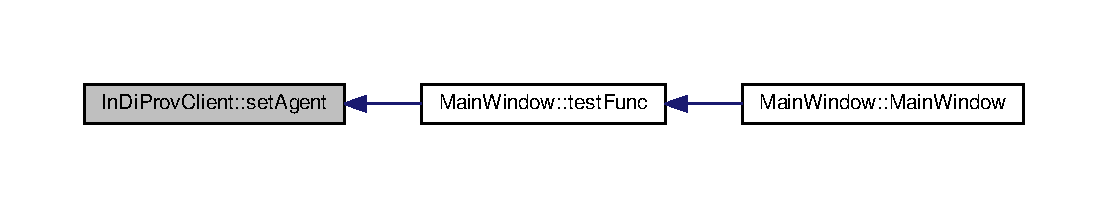
\includegraphics[width=350pt]{class_in_di_prov_client_a75ad36497b77b81841cf8cf411aea244_icgraph}
\end{center}
\end{figure}


\hypertarget{class_in_di_prov_client_abc388b71a141493921a6e51f18b60da8}{\index{In\-Di\-Prov\-Client@{In\-Di\-Prov\-Client}!set\-Entity@{set\-Entity}}
\index{set\-Entity@{set\-Entity}!InDiProvClient@{In\-Di\-Prov\-Client}}
\subsubsection[{set\-Entity}]{\setlength{\rightskip}{0pt plus 5cm}int In\-Di\-Prov\-Client\-::set\-Entity (
\begin{DoxyParamCaption}
\item[{string}]{label, }
\item[{string}]{location, }
\item[{string}]{type, }
\item[{string}]{val}
\end{DoxyParamCaption}
)}}\label{class_in_di_prov_client_abc388b71a141493921a6e51f18b60da8}


Creating new Entity returns the unique id of new Entity if the function is successful, else returns -\/1. 

An entity is a physical, digital, conceptual, or other kind of thing with some fixed aspects; entities may be real or imaginary.\par
 Example\-: An entity may be the document at I\-R\-I \href{http://www.bbc.co.uk/news/science-environment-17526723,}{\tt http\-://www.\-bbc.\-co.\-uk/news/science-\/environment-\/17526723,} a file in a file system, a car, or an idea. 

Here is the call graph for this function\-:
\nopagebreak
\begin{figure}[H]
\begin{center}
\leavevmode
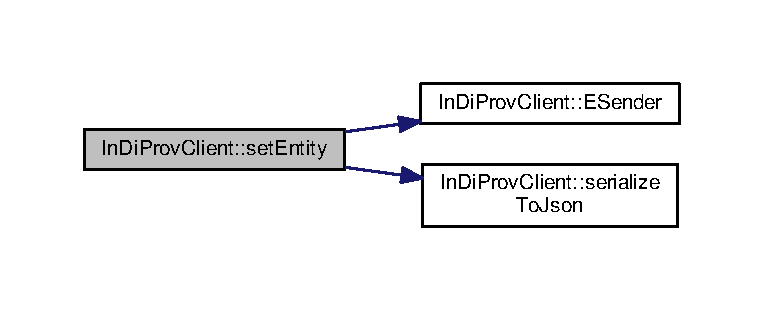
\includegraphics[width=350pt]{class_in_di_prov_client_abc388b71a141493921a6e51f18b60da8_cgraph}
\end{center}
\end{figure}




Here is the caller graph for this function\-:
\nopagebreak
\begin{figure}[H]
\begin{center}
\leavevmode
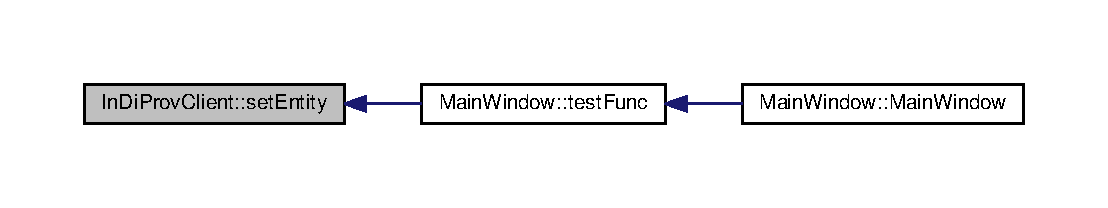
\includegraphics[width=350pt]{class_in_di_prov_client_abc388b71a141493921a6e51f18b60da8_icgraph}
\end{center}
\end{figure}


\hypertarget{class_in_di_prov_client_ae33d7a1a44e8d4e7ebbf832271938bce}{\index{In\-Di\-Prov\-Client@{In\-Di\-Prov\-Client}!setused@{setused}}
\index{setused@{setused}!InDiProvClient@{In\-Di\-Prov\-Client}}
\subsubsection[{setused}]{\setlength{\rightskip}{0pt plus 5cm}int In\-Di\-Prov\-Client\-::setused (
\begin{DoxyParamCaption}
\item[{int}]{act\-I\-D, }
\item[{int}]{ent\-I\-D, }
\item[{string}]{used\-Time, }
\item[{string}]{label, }
\item[{string}]{location, }
\item[{string}]{role, }
\item[{string}]{type}
\end{DoxyParamCaption}
)}}\label{class_in_di_prov_client_ae33d7a1a44e8d4e7ebbf832271938bce}


Creating new Usage returns the unique id of new usage if the function is successful, else returns -\/1. 

Activities and entities are associated with each other in two different ways\-: activities utilize entities and activities produce entities. The act of utilizing or producing an entity may have a duration. The term 'generation' refers to the completion of the act of producing; likewise, the term 'usage' refers to the beginning of the act of utilizing entities. Thus, we define the following concepts of generation and usage. Usage is the beginning of utilizing an entity by an activity. Before usage, the activity had not begun to utilize this entity and could not have been affected by the entity.\par
 Example 1\-: Usage examples include a procedure beginning to consume an argument, a service starting to read a value on a port, a program beginning to read a configuration file, or the point at which an ingredient, such as eggs, is being added in a baking activity. Usage may entirely consume an entity (e.\-g. eggs are no longer available after being added to the mix); in contrast, the same entity may be used multiple times, possibly by different activities (e.\-g. a file on a file system can be read indefinitely).\par
 Example 2\-: Let us consider the activity of driving a car from Boston to Cambridge. One might reasonably ask what entities are used and generated by this activity. This is answered by considering that a single artifact may correspond to several entities; in this case, a car in Boston may be a different entity from the same car in Cambridge. Thus, among other things, an entity \char`\"{}car in Boston\char`\"{} would be used, and a new entity \char`\"{}car in Cambridge\char`\"{} would be generated by this activity of driving. The provenance trace of the car might include\-: designed in Japan, manufactured in Korea, shipped to Boston U\-S\-A, purchased by customer, driven to Cambridge, serviced by engineer in Cambridge, etc., all of which might be important information when deciding whether or not it represents a sensible second-\/hand purchase. Or some of it might alternatively be relevant when trying to determine the truth of a web page reporting a traffic violation involving that car. This breadth of provenance allows descriptions of interactions between physical and digital artifacts. 

Here is the call graph for this function\-:
\nopagebreak
\begin{figure}[H]
\begin{center}
\leavevmode
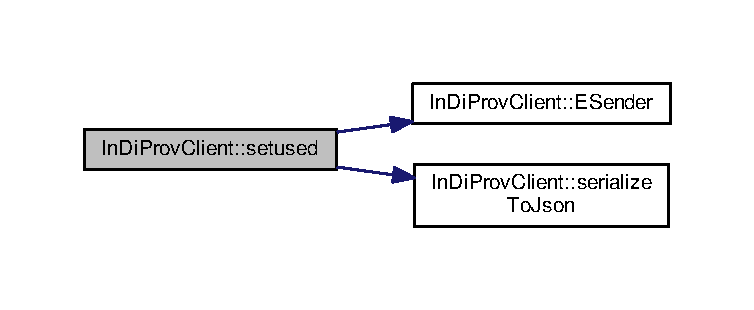
\includegraphics[width=350pt]{class_in_di_prov_client_ae33d7a1a44e8d4e7ebbf832271938bce_cgraph}
\end{center}
\end{figure}




Here is the caller graph for this function\-:
\nopagebreak
\begin{figure}[H]
\begin{center}
\leavevmode
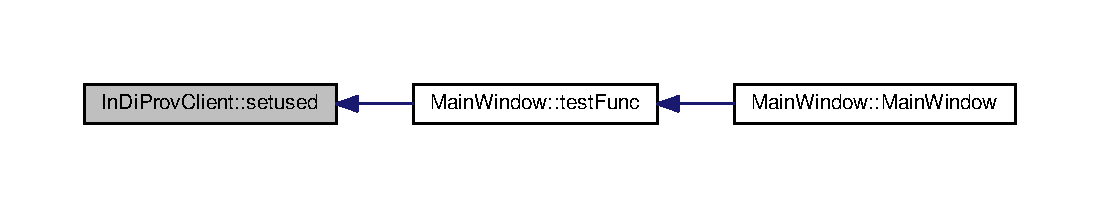
\includegraphics[width=350pt]{class_in_di_prov_client_ae33d7a1a44e8d4e7ebbf832271938bce_icgraph}
\end{center}
\end{figure}


\hypertarget{class_in_di_prov_client_a1a54aaeb77c6c4cca257999acf42d1e7}{\index{In\-Di\-Prov\-Client@{In\-Di\-Prov\-Client}!setwas\-Associated\-With@{setwas\-Associated\-With}}
\index{setwas\-Associated\-With@{setwas\-Associated\-With}!InDiProvClient@{In\-Di\-Prov\-Client}}
\subsubsection[{setwas\-Associated\-With}]{\setlength{\rightskip}{0pt plus 5cm}int In\-Di\-Prov\-Client\-::setwas\-Associated\-With (
\begin{DoxyParamCaption}
\item[{int}]{act\-I\-D, }
\item[{int}]{agent\-I\-D, }
\item[{int}]{plan\-I\-D, }
\item[{string}]{label, }
\item[{string}]{role, }
\item[{string}]{type}
\end{DoxyParamCaption}
)}}\label{class_in_di_prov_client_a1a54aaeb77c6c4cca257999acf42d1e7}


Creating new Association returns the unique id of new Association if the function is successful, else returns -\/1. 

Agents are defined as having some kind of responsibility for activities. An activity association is an assignment of responsibility to an agent for an activity, indicating that the agent had a role in the activity.\par
 Example\-: Examples of association between an activity and an agent are\-:\par
 creation of a web page under the guidance of a designer;\par
 various forms of participation in a panel discussion, including audience member, panelist, or panel chair;\par
 a public event, sponsored by a company, and hosted by a museum;\par
 

Here is the call graph for this function\-:
\nopagebreak
\begin{figure}[H]
\begin{center}
\leavevmode
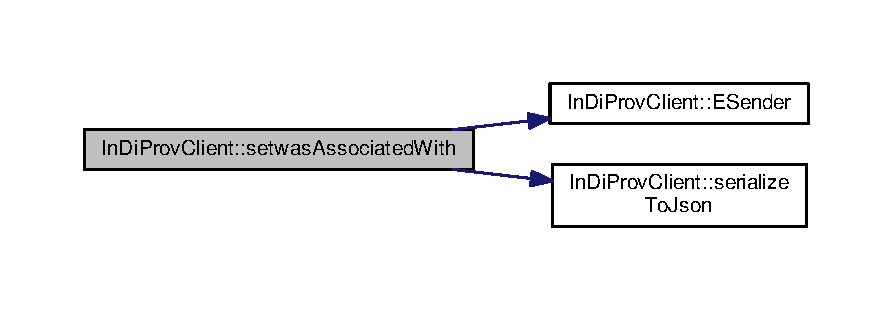
\includegraphics[width=350pt]{class_in_di_prov_client_a1a54aaeb77c6c4cca257999acf42d1e7_cgraph}
\end{center}
\end{figure}




Here is the caller graph for this function\-:
\nopagebreak
\begin{figure}[H]
\begin{center}
\leavevmode
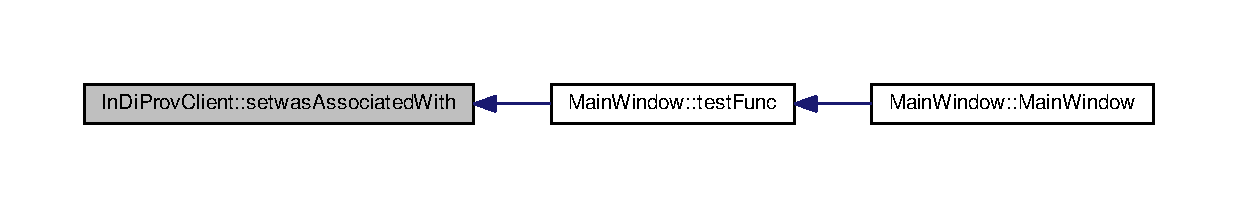
\includegraphics[width=350pt]{class_in_di_prov_client_a1a54aaeb77c6c4cca257999acf42d1e7_icgraph}
\end{center}
\end{figure}


\hypertarget{class_in_di_prov_client_ac57311b22c1378f8f542e91c4285f935}{\index{In\-Di\-Prov\-Client@{In\-Di\-Prov\-Client}!setwas\-Attributed\-To@{setwas\-Attributed\-To}}
\index{setwas\-Attributed\-To@{setwas\-Attributed\-To}!InDiProvClient@{In\-Di\-Prov\-Client}}
\subsubsection[{setwas\-Attributed\-To}]{\setlength{\rightskip}{0pt plus 5cm}int In\-Di\-Prov\-Client\-::setwas\-Attributed\-To (
\begin{DoxyParamCaption}
\item[{int}]{ent\-I\-D, }
\item[{int}]{agent\-I\-D, }
\item[{string}]{label, }
\item[{string}]{type}
\end{DoxyParamCaption}
)}}\label{class_in_di_prov_client_ac57311b22c1378f8f542e91c4285f935}


Creating new Attribution returns the unique id of new Attribution if the function is successful, else returns -\/1. 

Agents can be related to entities, activities, and other agents. Attribution is the ascribing of an entity to an agent.\par
 Example\-: E\-A blog post can be attributed to an author, a mobile phone to its manufacturer.\par
 

Here is the call graph for this function\-:
\nopagebreak
\begin{figure}[H]
\begin{center}
\leavevmode
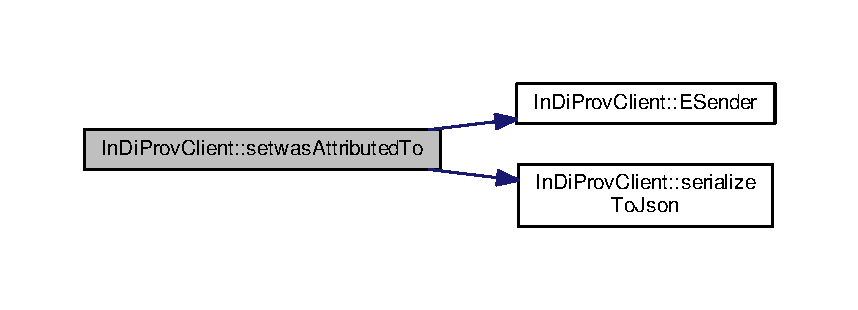
\includegraphics[width=350pt]{class_in_di_prov_client_ac57311b22c1378f8f542e91c4285f935_cgraph}
\end{center}
\end{figure}




Here is the caller graph for this function\-:
\nopagebreak
\begin{figure}[H]
\begin{center}
\leavevmode
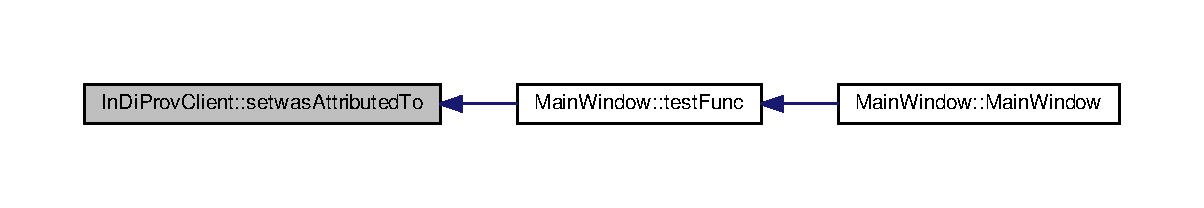
\includegraphics[width=350pt]{class_in_di_prov_client_ac57311b22c1378f8f542e91c4285f935_icgraph}
\end{center}
\end{figure}


\hypertarget{class_in_di_prov_client_afc085d595289e66d9b3928e9a4229051}{\index{In\-Di\-Prov\-Client@{In\-Di\-Prov\-Client}!setwas\-Derived\-From@{setwas\-Derived\-From}}
\index{setwas\-Derived\-From@{setwas\-Derived\-From}!InDiProvClient@{In\-Di\-Prov\-Client}}
\subsubsection[{setwas\-Derived\-From}]{\setlength{\rightskip}{0pt plus 5cm}int In\-Di\-Prov\-Client\-::setwas\-Derived\-From (
\begin{DoxyParamCaption}
\item[{int}]{gen\-Ent\-I\-D, }
\item[{int}]{usd\-Ent\-I\-D, }
\item[{int}]{act\-I\-D, }
\item[{int}]{gen\-I\-D, }
\item[{int}]{usg\-I\-D, }
\item[{string}]{label, }
\item[{string}]{type}
\end{DoxyParamCaption}
)}}\label{class_in_di_prov_client_afc085d595289e66d9b3928e9a4229051}


Creating new Derivation returns the unique id of new Derivation if the function is successful, else returns -\/1. 

Activities utilize entities and produce entities. In some cases, utilizing an entity influences the creation of another in some way. This notion of 'influence' is captured by derivations, defined as follows. A derivation is a transformation of an entity into another, an update of an entity resulting in a new one, or the construction of a new entity based on a pre-\/existing entity.\par
 Example\-: Examples of derivation include the transformation of a relational table into a linked data set, the transformation of a canvas into a painting, the transportation of a work of art from London to New York, and a physical transformation such as the melting of ice into water.\par
 The focus of derivation is on connecting a generated entity to a used entity. While the basic idea is simple, the concept of derivation can be quite subtle\-: implicit is the notion that the generated entity was affected in some way by the used entity. If an artifact was used by an activity that also generated a new artifact, it does not always follow that the second artifact was derived from the first. In the activity of creating a painting, an artist may have mixed some paint that was never actually applied to the canvas\-: the painting would typically not be considered a derivation from the unused paint. P\-R\-O\-V does not attempt to specify the conditions under which derivations exist; rather, derivation is considered to have been determined by unspecified means. Thus, while a chain of usage and generation is necessary for a derivation to hold between entities, it is not sufficient; some form of influence occurring during the activities involved is also needed. 

Here is the call graph for this function\-:
\nopagebreak
\begin{figure}[H]
\begin{center}
\leavevmode
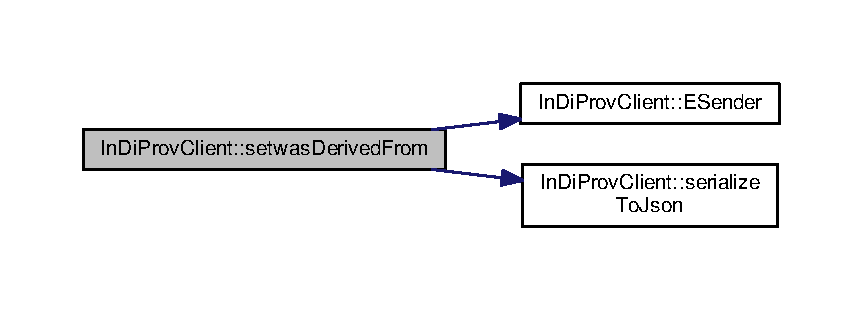
\includegraphics[width=350pt]{class_in_di_prov_client_afc085d595289e66d9b3928e9a4229051_cgraph}
\end{center}
\end{figure}




Here is the caller graph for this function\-:
\nopagebreak
\begin{figure}[H]
\begin{center}
\leavevmode
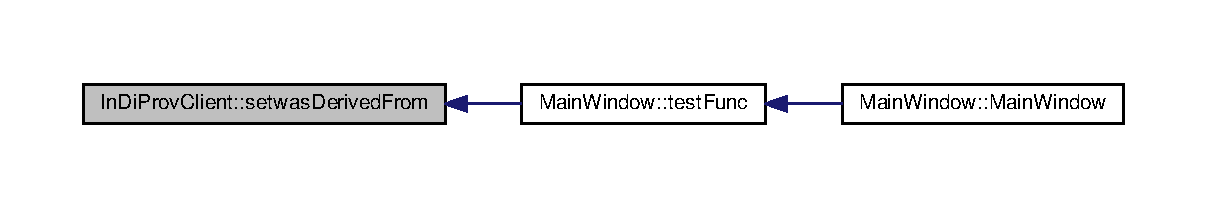
\includegraphics[width=350pt]{class_in_di_prov_client_afc085d595289e66d9b3928e9a4229051_icgraph}
\end{center}
\end{figure}


\hypertarget{class_in_di_prov_client_aecb51b066ab1096fc095b00ec6e04c8b}{\index{In\-Di\-Prov\-Client@{In\-Di\-Prov\-Client}!setwas\-Ended\-By@{setwas\-Ended\-By}}
\index{setwas\-Ended\-By@{setwas\-Ended\-By}!InDiProvClient@{In\-Di\-Prov\-Client}}
\subsubsection[{setwas\-Ended\-By}]{\setlength{\rightskip}{0pt plus 5cm}int In\-Di\-Prov\-Client\-::setwas\-Ended\-By (
\begin{DoxyParamCaption}
\item[{int}]{act\-I\-D, }
\item[{int}]{ent\-I\-D, }
\item[{int}]{ender\-Act\-I\-D, }
\item[{string}]{e\-Time, }
\item[{string}]{label, }
\item[{string}]{location, }
\item[{string}]{role, }
\item[{string}]{type}
\end{DoxyParamCaption}
)}}\label{class_in_di_prov_client_aecb51b066ab1096fc095b00ec6e04c8b}


Creating new returns the unique id of new if the function is successful, else returns -\/1. 

End is when an activity is deemed to have been ended by an entity, known as trigger. The activity no longer exists after its end. Any usage, generation, or invalidation involving an activity precedes the activity's end. An end may refer to a trigger entity that terminated the activity, or to an activity, known as ender that generated the trigger. 

Here is the call graph for this function\-:
\nopagebreak
\begin{figure}[H]
\begin{center}
\leavevmode
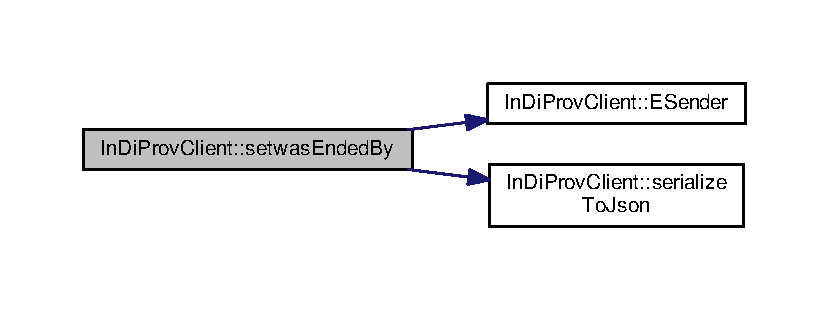
\includegraphics[width=350pt]{class_in_di_prov_client_aecb51b066ab1096fc095b00ec6e04c8b_cgraph}
\end{center}
\end{figure}




Here is the caller graph for this function\-:
\nopagebreak
\begin{figure}[H]
\begin{center}
\leavevmode
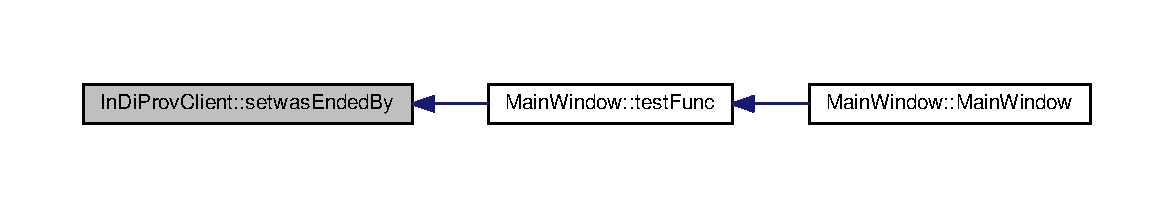
\includegraphics[width=350pt]{class_in_di_prov_client_aecb51b066ab1096fc095b00ec6e04c8b_icgraph}
\end{center}
\end{figure}


\hypertarget{class_in_di_prov_client_a30aa922f818e6a6104185c9a11191acb}{\index{In\-Di\-Prov\-Client@{In\-Di\-Prov\-Client}!setwas\-Generated\-By@{setwas\-Generated\-By}}
\index{setwas\-Generated\-By@{setwas\-Generated\-By}!InDiProvClient@{In\-Di\-Prov\-Client}}
\subsubsection[{setwas\-Generated\-By}]{\setlength{\rightskip}{0pt plus 5cm}int In\-Di\-Prov\-Client\-::setwas\-Generated\-By (
\begin{DoxyParamCaption}
\item[{int}]{ent\-I\-D, }
\item[{int}]{act\-I\-D, }
\item[{string}]{generate\-Time, }
\item[{string}]{label, }
\item[{string}]{location, }
\item[{string}]{role, }
\item[{string}]{type}
\end{DoxyParamCaption}
)}}\label{class_in_di_prov_client_a30aa922f818e6a6104185c9a11191acb}


Creating new Generation returns the unique id of new Generation if the function is successful, else returns -\/1. 

Activities and entities are associated with each other in two different ways\-: activities utilize entities and activities produce entities. The act of utilizing or producing an entity may have a duration. The term 'generation' refers to the completion of the act of producing; likewise, the term 'usage' refers to the beginning of the act of utilizing entities. Thus, we define the following concepts of generation and usage. Generation is the completion of production of a new entity by an activity. This entity did not exist before generation and becomes available for usage after this generation.\par
 Example\-: Examples of generation are the completed creation of a file by a program, the completed creation of a linked data set, and the completed publication of a new version of a document. 

Here is the call graph for this function\-:
\nopagebreak
\begin{figure}[H]
\begin{center}
\leavevmode
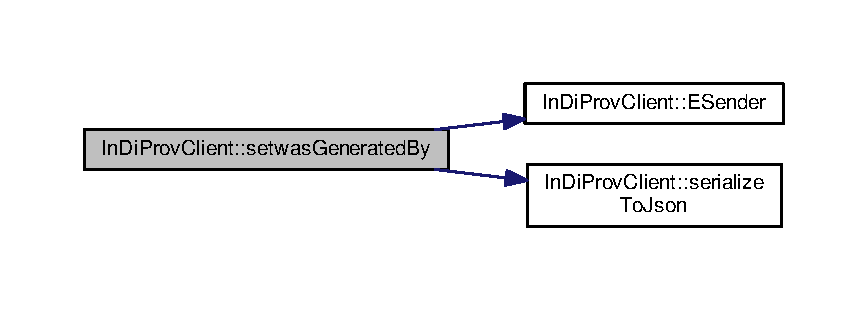
\includegraphics[width=350pt]{class_in_di_prov_client_a30aa922f818e6a6104185c9a11191acb_cgraph}
\end{center}
\end{figure}




Here is the caller graph for this function\-:
\nopagebreak
\begin{figure}[H]
\begin{center}
\leavevmode
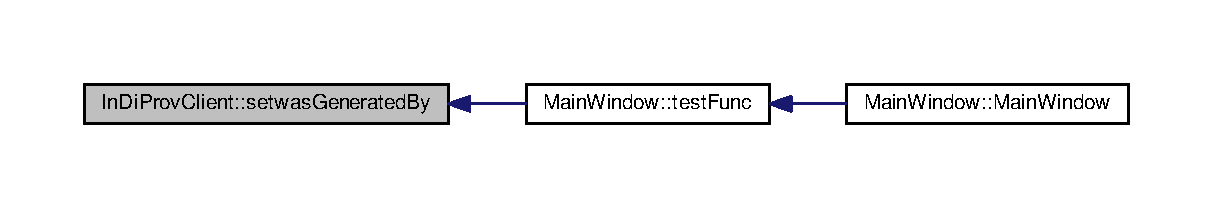
\includegraphics[width=350pt]{class_in_di_prov_client_a30aa922f818e6a6104185c9a11191acb_icgraph}
\end{center}
\end{figure}


\hypertarget{class_in_di_prov_client_aa9fbfb3480eded57485c9d4585375625}{\index{In\-Di\-Prov\-Client@{In\-Di\-Prov\-Client}!setwas\-Informed\-By@{setwas\-Informed\-By}}
\index{setwas\-Informed\-By@{setwas\-Informed\-By}!InDiProvClient@{In\-Di\-Prov\-Client}}
\subsubsection[{setwas\-Informed\-By}]{\setlength{\rightskip}{0pt plus 5cm}int In\-Di\-Prov\-Client\-::setwas\-Informed\-By (
\begin{DoxyParamCaption}
\item[{int}]{informed, }
\item[{int}]{informant, }
\item[{string}]{label, }
\item[{string}]{type}
\end{DoxyParamCaption}
)}}\label{class_in_di_prov_client_aa9fbfb3480eded57485c9d4585375625}


Creating new Communication returns the unique id of new Communication if the function is successful, else returns -\/1. 

The generation of an entity by an activity and its subsequent usage by another activity is termed communication. Communication is the exchange of some unspecified entity by two activities, one activity using some entity generated by the other.\par
 Example\-: The activity of writing a celebrity article was informed by (a communication instance) the activity of intercepting voicemails. 

Here is the call graph for this function\-:
\nopagebreak
\begin{figure}[H]
\begin{center}
\leavevmode
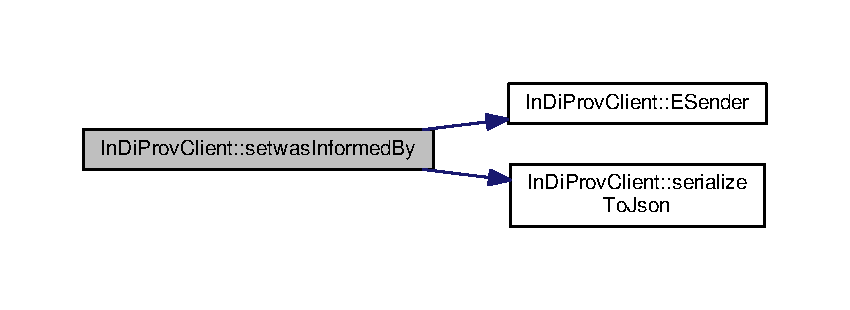
\includegraphics[width=350pt]{class_in_di_prov_client_aa9fbfb3480eded57485c9d4585375625_cgraph}
\end{center}
\end{figure}




Here is the caller graph for this function\-:
\nopagebreak
\begin{figure}[H]
\begin{center}
\leavevmode
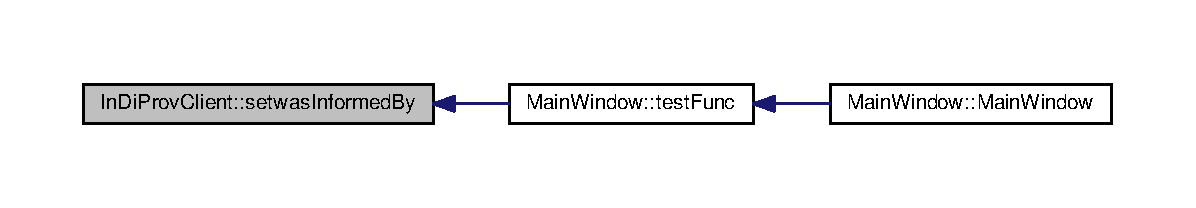
\includegraphics[width=350pt]{class_in_di_prov_client_aa9fbfb3480eded57485c9d4585375625_icgraph}
\end{center}
\end{figure}


\hypertarget{class_in_di_prov_client_a05a450e338417ff0966bba635834f64a}{\index{In\-Di\-Prov\-Client@{In\-Di\-Prov\-Client}!setwas\-Started\-By@{setwas\-Started\-By}}
\index{setwas\-Started\-By@{setwas\-Started\-By}!InDiProvClient@{In\-Di\-Prov\-Client}}
\subsubsection[{setwas\-Started\-By}]{\setlength{\rightskip}{0pt plus 5cm}int In\-Di\-Prov\-Client\-::setwas\-Started\-By (
\begin{DoxyParamCaption}
\item[{int}]{act\-I\-D, }
\item[{int}]{ent\-I\-D, }
\item[{int}]{starter\-Act\-I\-D, }
\item[{string}]{s\-Time, }
\item[{string}]{label, }
\item[{string}]{location, }
\item[{string}]{role, }
\item[{string}]{type}
\end{DoxyParamCaption}
)}}\label{class_in_di_prov_client_a05a450e338417ff0966bba635834f64a}


Creating new Start returns the unique id of new Start if the function is successful, else returns -\/1. 

Start is when an activity is deemed to have been started by an entity, known as trigger. The activity did not exist before its start. Any usage, generation, or invalidation involving an activity follows the activity's start. A start may refer to a trigger entity that set off the activity, or to an activity, known as starter, that generated the trigger. 

Here is the call graph for this function\-:
\nopagebreak
\begin{figure}[H]
\begin{center}
\leavevmode
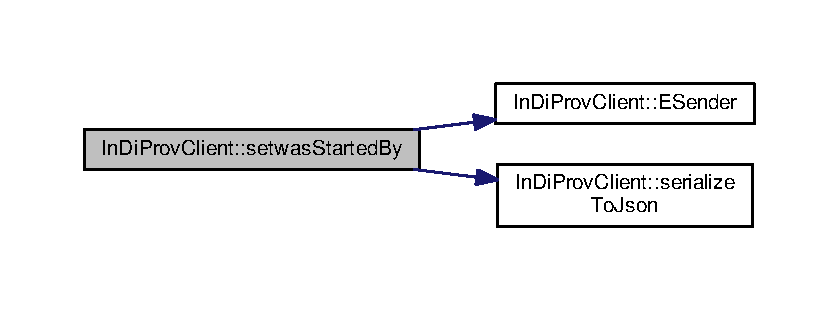
\includegraphics[width=350pt]{class_in_di_prov_client_a05a450e338417ff0966bba635834f64a_cgraph}
\end{center}
\end{figure}




Here is the caller graph for this function\-:
\nopagebreak
\begin{figure}[H]
\begin{center}
\leavevmode
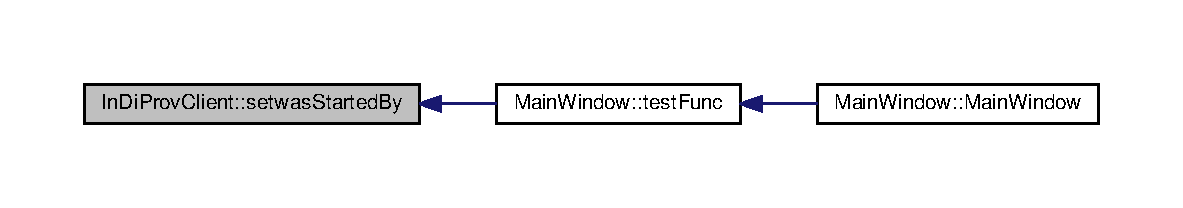
\includegraphics[width=350pt]{class_in_di_prov_client_a05a450e338417ff0966bba635834f64a_icgraph}
\end{center}
\end{figure}




The documentation for this class was generated from the following files\-:\begin{DoxyCompactItemize}
\item 
\hyperlink{indiprovclient_8h}{indiprovclient.\-h}\item 
\hyperlink{indiprovclient_8cpp}{indiprovclient.\-cpp}\end{DoxyCompactItemize}

\hypertarget{class_main_window}{\section{Main\-Window Class Reference}
\label{class_main_window}\index{Main\-Window@{Main\-Window}}
}


{\ttfamily \#include $<$mainwindow.\-h$>$}



Inheritance diagram for Main\-Window\-:
\nopagebreak
\begin{figure}[H]
\begin{center}
\leavevmode
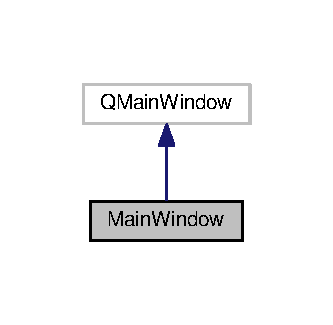
\includegraphics[width=160pt]{class_main_window__inherit__graph}
\end{center}
\end{figure}


Collaboration diagram for Main\-Window\-:
\nopagebreak
\begin{figure}[H]
\begin{center}
\leavevmode
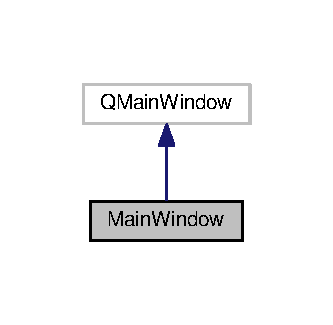
\includegraphics[width=160pt]{class_main_window__coll__graph}
\end{center}
\end{figure}
\subsection*{Public Member Functions}
\begin{DoxyCompactItemize}
\item 
\hyperlink{class_main_window_a8b244be8b7b7db1b08de2a2acb9409db}{Main\-Window} (Q\-Widget $\ast$parent=0)
\item 
\hyperlink{class_main_window_ae98d00a93bc118200eeef9f9bba1dba7}{$\sim$\-Main\-Window} ()
\item 
void \hyperlink{class_main_window_a3d5cb165efb53da512f94288d9257168}{E\-Sender} (zmq\-::context\-\_\-t $\ast$context, vector$<$ string $>$ mycmd)
\item 
string \hyperlink{class_main_window_a92901009572885892658ab2e8d7bb191}{serialize\-To\-Json} (vector$<$ string $>$ command\-Vec)
\item 
void \hyperlink{class_main_window_a9bc89dd1034e410e99a9e3f82cb032b3}{json\-\_\-parse} (json\-\_\-object $\ast$jobj)
\item 
void \hyperlink{class_main_window_ae4b6bf5d06819fab861e9e99b5a88699}{test\-Func} ()
\end{DoxyCompactItemize}


\subsection{Constructor \& Destructor Documentation}
\hypertarget{class_main_window_a8b244be8b7b7db1b08de2a2acb9409db}{\index{Main\-Window@{Main\-Window}!Main\-Window@{Main\-Window}}
\index{Main\-Window@{Main\-Window}!MainWindow@{Main\-Window}}
\subsubsection[{Main\-Window}]{\setlength{\rightskip}{0pt plus 5cm}Main\-Window\-::\-Main\-Window (
\begin{DoxyParamCaption}
\item[{Q\-Widget $\ast$}]{parent = {\ttfamily 0}}
\end{DoxyParamCaption}
)\hspace{0.3cm}{\ttfamily [explicit]}}}\label{class_main_window_a8b244be8b7b7db1b08de2a2acb9409db}


Here is the call graph for this function\-:
\nopagebreak
\begin{figure}[H]
\begin{center}
\leavevmode
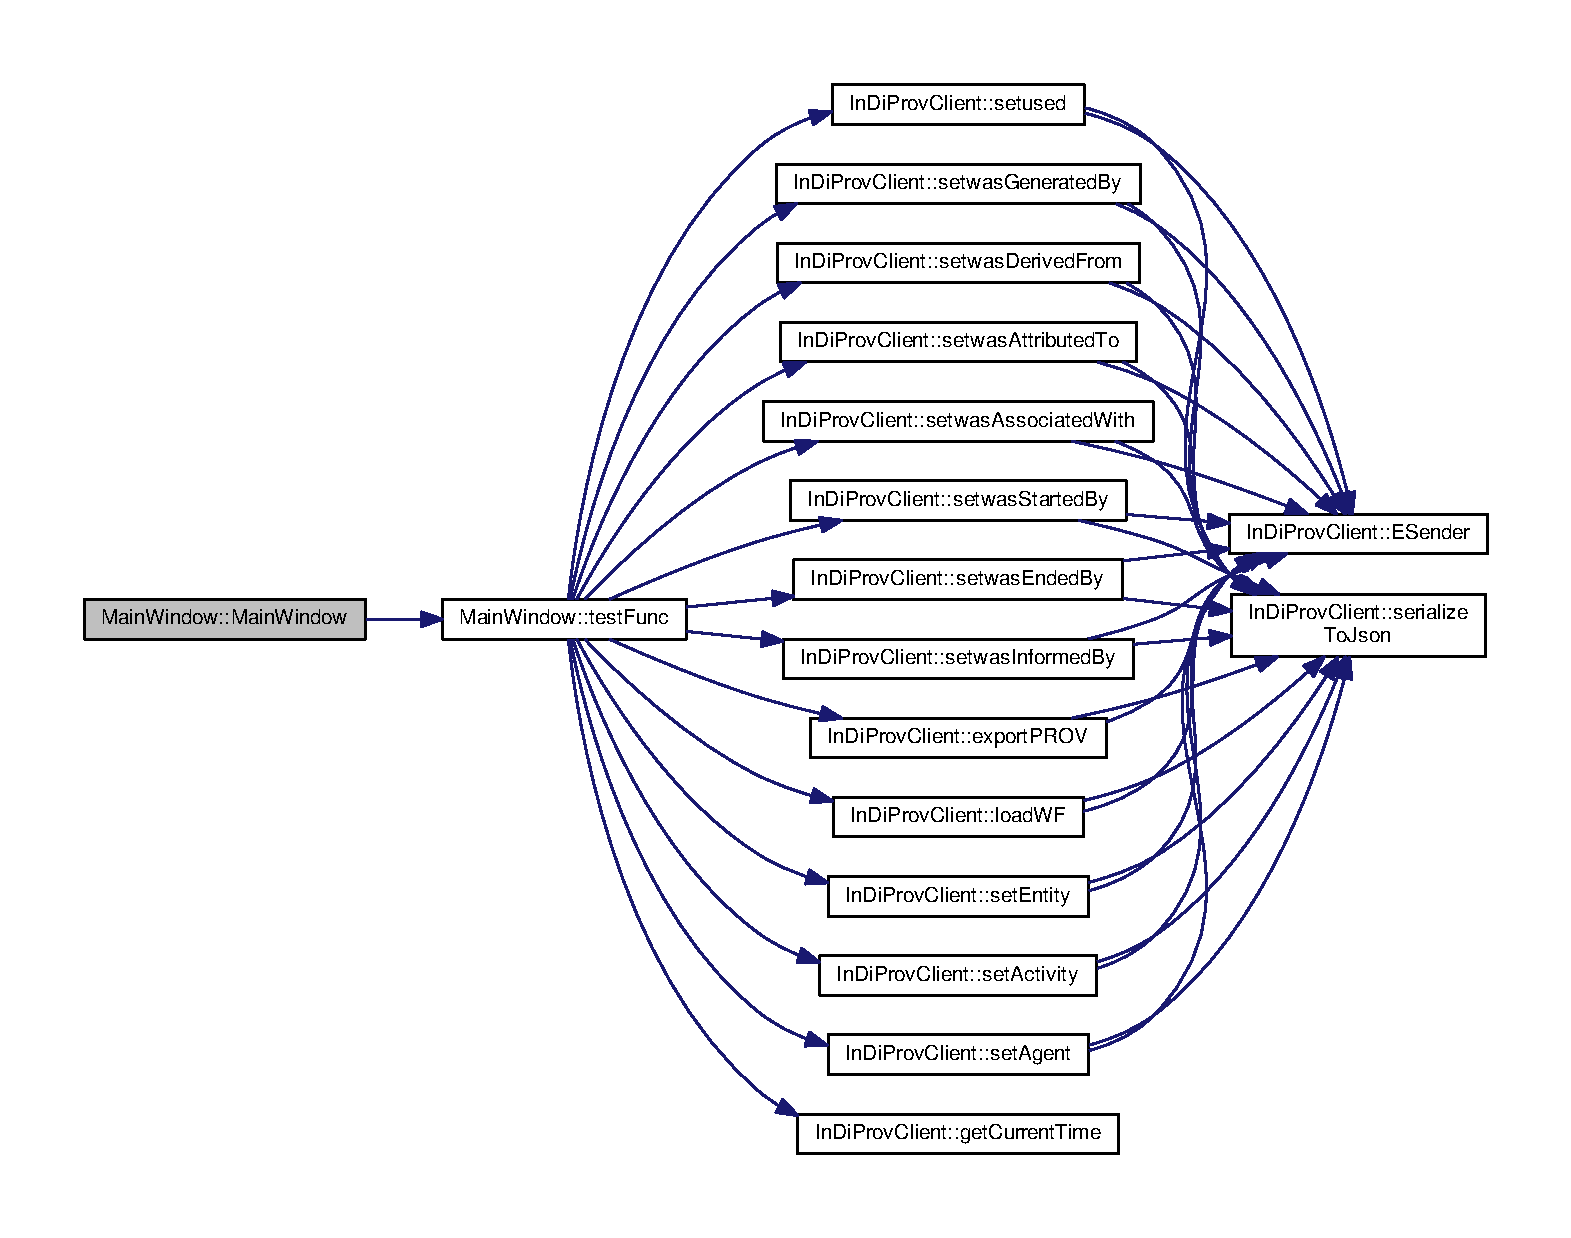
\includegraphics[width=350pt]{class_main_window_a8b244be8b7b7db1b08de2a2acb9409db_cgraph}
\end{center}
\end{figure}


\hypertarget{class_main_window_ae98d00a93bc118200eeef9f9bba1dba7}{\index{Main\-Window@{Main\-Window}!$\sim$\-Main\-Window@{$\sim$\-Main\-Window}}
\index{$\sim$\-Main\-Window@{$\sim$\-Main\-Window}!MainWindow@{Main\-Window}}
\subsubsection[{$\sim$\-Main\-Window}]{\setlength{\rightskip}{0pt plus 5cm}Main\-Window\-::$\sim$\-Main\-Window (
\begin{DoxyParamCaption}
{}
\end{DoxyParamCaption}
)}}\label{class_main_window_ae98d00a93bc118200eeef9f9bba1dba7}


\subsection{Member Function Documentation}
\hypertarget{class_main_window_a3d5cb165efb53da512f94288d9257168}{\index{Main\-Window@{Main\-Window}!E\-Sender@{E\-Sender}}
\index{E\-Sender@{E\-Sender}!MainWindow@{Main\-Window}}
\subsubsection[{E\-Sender}]{\setlength{\rightskip}{0pt plus 5cm}void Main\-Window\-::\-E\-Sender (
\begin{DoxyParamCaption}
\item[{zmq\-::context\-\_\-t $\ast$}]{context, }
\item[{vector$<$ string $>$}]{mycmd}
\end{DoxyParamCaption}
)}}\label{class_main_window_a3d5cb165efb53da512f94288d9257168}


Here is the call graph for this function\-:
\nopagebreak
\begin{figure}[H]
\begin{center}
\leavevmode
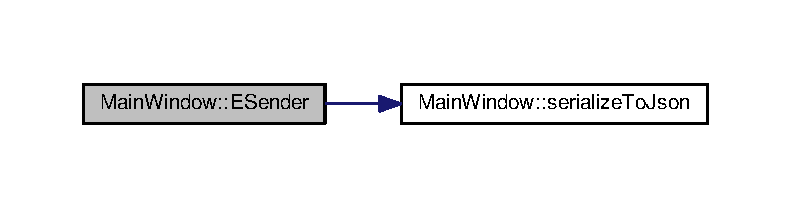
\includegraphics[width=350pt]{class_main_window_a3d5cb165efb53da512f94288d9257168_cgraph}
\end{center}
\end{figure}


\hypertarget{class_main_window_a9bc89dd1034e410e99a9e3f82cb032b3}{\index{Main\-Window@{Main\-Window}!json\-\_\-parse@{json\-\_\-parse}}
\index{json\-\_\-parse@{json\-\_\-parse}!MainWindow@{Main\-Window}}
\subsubsection[{json\-\_\-parse}]{\setlength{\rightskip}{0pt plus 5cm}void Main\-Window\-::json\-\_\-parse (
\begin{DoxyParamCaption}
\item[{json\-\_\-object $\ast$}]{jobj}
\end{DoxyParamCaption}
)}}\label{class_main_window_a9bc89dd1034e410e99a9e3f82cb032b3}
\hypertarget{class_main_window_a92901009572885892658ab2e8d7bb191}{\index{Main\-Window@{Main\-Window}!serialize\-To\-Json@{serialize\-To\-Json}}
\index{serialize\-To\-Json@{serialize\-To\-Json}!MainWindow@{Main\-Window}}
\subsubsection[{serialize\-To\-Json}]{\setlength{\rightskip}{0pt plus 5cm}string Main\-Window\-::serialize\-To\-Json (
\begin{DoxyParamCaption}
\item[{vector$<$ string $>$}]{command\-Vec}
\end{DoxyParamCaption}
)}}\label{class_main_window_a92901009572885892658ab2e8d7bb191}


Here is the caller graph for this function\-:
\nopagebreak
\begin{figure}[H]
\begin{center}
\leavevmode
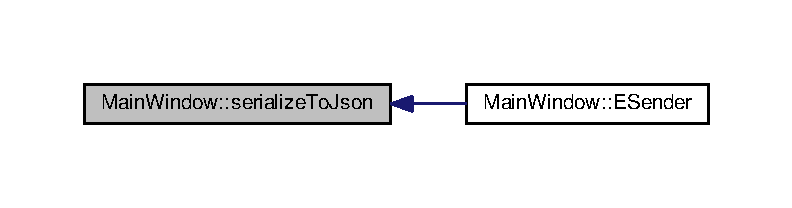
\includegraphics[width=350pt]{class_main_window_a92901009572885892658ab2e8d7bb191_icgraph}
\end{center}
\end{figure}


\hypertarget{class_main_window_ae4b6bf5d06819fab861e9e99b5a88699}{\index{Main\-Window@{Main\-Window}!test\-Func@{test\-Func}}
\index{test\-Func@{test\-Func}!MainWindow@{Main\-Window}}
\subsubsection[{test\-Func}]{\setlength{\rightskip}{0pt plus 5cm}void Main\-Window\-::test\-Func (
\begin{DoxyParamCaption}
{}
\end{DoxyParamCaption}
)}}\label{class_main_window_ae4b6bf5d06819fab861e9e99b5a88699}


Here is the call graph for this function\-:
\nopagebreak
\begin{figure}[H]
\begin{center}
\leavevmode
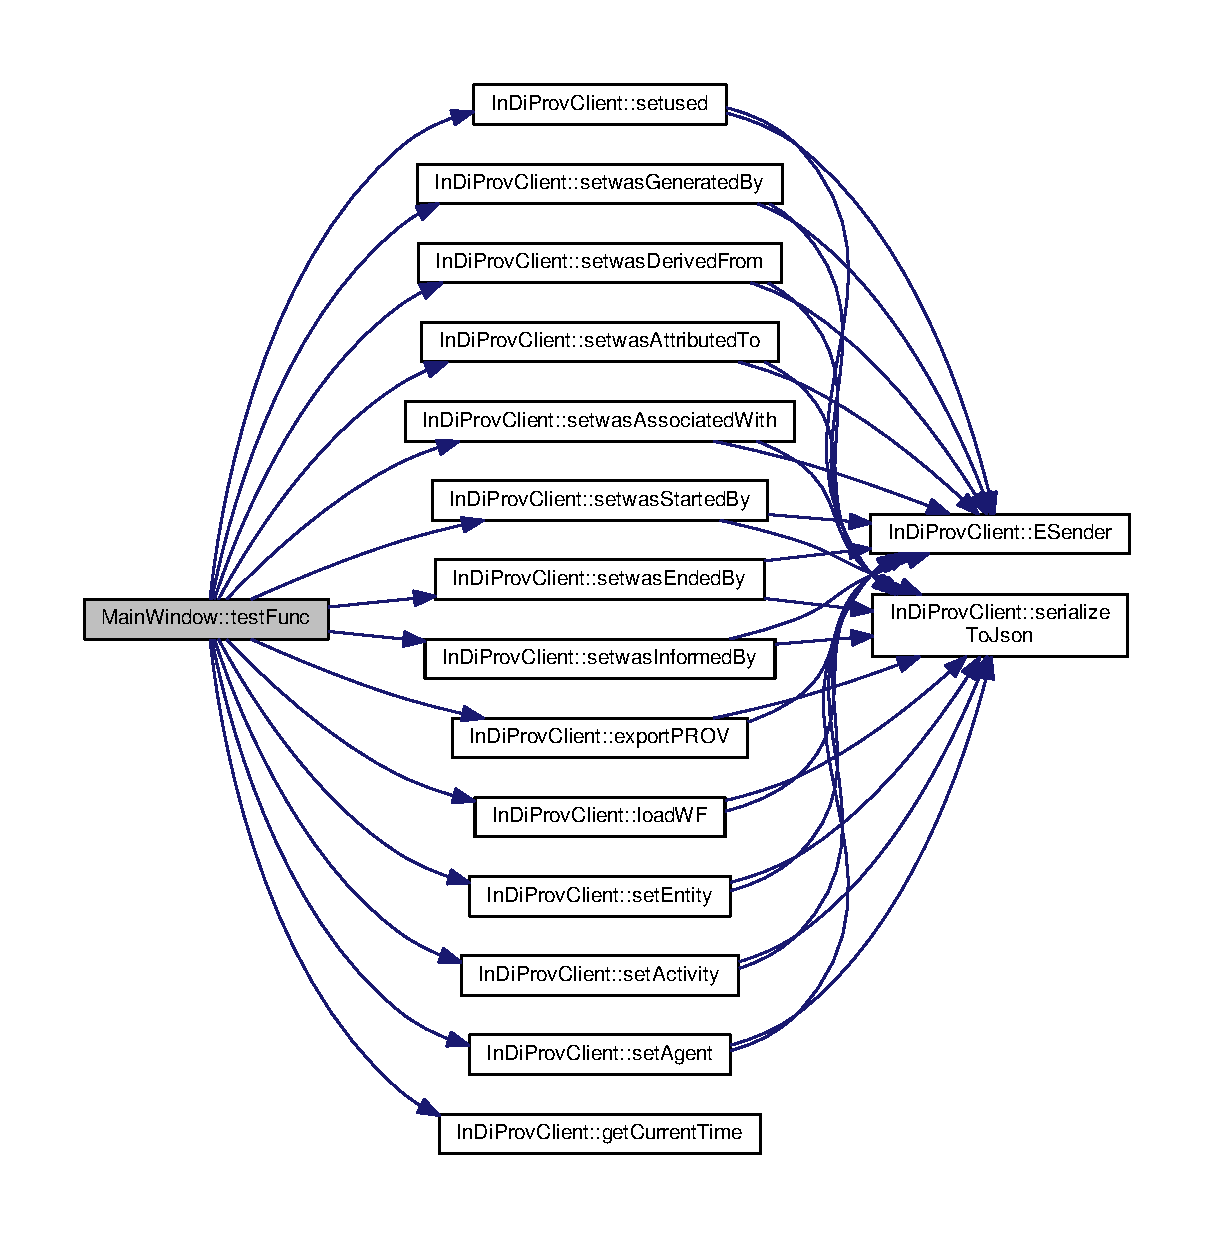
\includegraphics[width=350pt]{class_main_window_ae4b6bf5d06819fab861e9e99b5a88699_cgraph}
\end{center}
\end{figure}




Here is the caller graph for this function\-:
\nopagebreak
\begin{figure}[H]
\begin{center}
\leavevmode
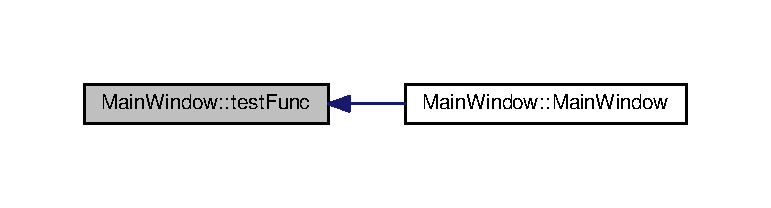
\includegraphics[width=350pt]{class_main_window_ae4b6bf5d06819fab861e9e99b5a88699_icgraph}
\end{center}
\end{figure}




The documentation for this class was generated from the following files\-:\begin{DoxyCompactItemize}
\item 
\hyperlink{mainwindow_8h}{mainwindow.\-h}\item 
\hyperlink{mainwindow_8cpp}{mainwindow.\-cpp}\end{DoxyCompactItemize}

\hypertarget{classmsg_parsing}{\section{msg\-Parsing Class Reference}
\label{classmsg_parsing}\index{msg\-Parsing@{msg\-Parsing}}
}


{\ttfamily \#include $<$msgparsing.\-h$>$}

\subsection*{Public Member Functions}
\begin{DoxyCompactItemize}
\item 
\hyperlink{classmsg_parsing_a010960ce78f09282b8d34ca4632060a7}{msg\-Parsing} ()
\end{DoxyCompactItemize}


\subsection{Constructor \& Destructor Documentation}
\hypertarget{classmsg_parsing_a010960ce78f09282b8d34ca4632060a7}{\index{msg\-Parsing@{msg\-Parsing}!msg\-Parsing@{msg\-Parsing}}
\index{msg\-Parsing@{msg\-Parsing}!msgParsing@{msg\-Parsing}}
\subsubsection[{msg\-Parsing}]{\setlength{\rightskip}{0pt plus 5cm}msg\-Parsing\-::msg\-Parsing (
\begin{DoxyParamCaption}
{}
\end{DoxyParamCaption}
)}}\label{classmsg_parsing_a010960ce78f09282b8d34ca4632060a7}


The documentation for this class was generated from the following files\-:\begin{DoxyCompactItemize}
\item 
\hyperlink{msgparsing_8h}{msgparsing.\-h}\item 
\hyperlink{msgparsing_8cpp}{msgparsing.\-cpp}\end{DoxyCompactItemize}

\hypertarget{structmyteststruct}{\section{myteststruct Struct Reference}
\label{structmyteststruct}\index{myteststruct@{myteststruct}}
}
\subsection*{Public Attributes}
\begin{DoxyCompactItemize}
\item 
int \hyperlink{structmyteststruct_a2a25e3e82c3ec8e4c9e2a6f6abe6a746}{x}
\item 
int \hyperlink{structmyteststruct_ade0ef34f12443469bad8641334c5931f}{y}
\item 
int \hyperlink{structmyteststruct_ad619e93b64c7295d8bb126ee2402372e}{z}
\end{DoxyCompactItemize}


\subsection{Member Data Documentation}
\hypertarget{structmyteststruct_a2a25e3e82c3ec8e4c9e2a6f6abe6a746}{\index{myteststruct@{myteststruct}!x@{x}}
\index{x@{x}!myteststruct@{myteststruct}}
\subsubsection[{x}]{\setlength{\rightskip}{0pt plus 5cm}int myteststruct\-::x}}\label{structmyteststruct_a2a25e3e82c3ec8e4c9e2a6f6abe6a746}
\hypertarget{structmyteststruct_ade0ef34f12443469bad8641334c5931f}{\index{myteststruct@{myteststruct}!y@{y}}
\index{y@{y}!myteststruct@{myteststruct}}
\subsubsection[{y}]{\setlength{\rightskip}{0pt plus 5cm}int myteststruct\-::y}}\label{structmyteststruct_ade0ef34f12443469bad8641334c5931f}
\hypertarget{structmyteststruct_ad619e93b64c7295d8bb126ee2402372e}{\index{myteststruct@{myteststruct}!z@{z}}
\index{z@{z}!myteststruct@{myteststruct}}
\subsubsection[{z}]{\setlength{\rightskip}{0pt plus 5cm}int myteststruct\-::z}}\label{structmyteststruct_ad619e93b64c7295d8bb126ee2402372e}


The documentation for this struct was generated from the following file\-:\begin{DoxyCompactItemize}
\item 
\hyperlink{mainwindow_8cpp}{mainwindow.\-cpp}\end{DoxyCompactItemize}

\hypertarget{class_prov_utils}{\section{Prov\-Utils Class Reference}
\label{class_prov_utils}\index{Prov\-Utils@{Prov\-Utils}}
}


{\ttfamily \#include $<$provutils.\-h$>$}

\subsection*{Classes}
\begin{DoxyCompactItemize}
\item 
struct \hyperlink{struct_prov_utils_1_1_activity}{Activity}
\item 
struct \hyperlink{struct_prov_utils_1_1_agent}{Agent}
\item 
struct \hyperlink{struct_prov_utils_1_1_entity}{Entity}
\item 
struct \hyperlink{struct_prov_utils_1_1_used}{Used}
\item 
struct \hyperlink{struct_prov_utils_1_1_was_associated_with}{Was\-Associated\-With}
\item 
struct \hyperlink{struct_prov_utils_1_1_was_attributed_to}{Was\-Attributed\-To}
\item 
struct \hyperlink{struct_prov_utils_1_1_was_derived_from}{Was\-Derived\-From}
\item 
struct \hyperlink{struct_prov_utils_1_1_was_ended_by}{Was\-Ended\-By}
\item 
struct \hyperlink{struct_prov_utils_1_1_was_generated_by}{Was\-Generated\-By}
\item 
struct \hyperlink{struct_prov_utils_1_1_was_informed_by}{Was\-Informed\-By}
\item 
struct \hyperlink{struct_prov_utils_1_1_was_started_by}{Was\-Started\-By}
\end{DoxyCompactItemize}
\subsection*{Public Member Functions}
\begin{DoxyCompactItemize}
\item 
\hyperlink{class_prov_utils_a1c050ce900080f4b2bf9731b7799c025}{Prov\-Utils} ()
\item 
\hyperlink{class_prov_utils_aef1d5cc117ebf195fc29cb85719ec0f0}{$\sim$\-Prov\-Utils} ()
\end{DoxyCompactItemize}


\subsection{Constructor \& Destructor Documentation}
\hypertarget{class_prov_utils_a1c050ce900080f4b2bf9731b7799c025}{\index{Prov\-Utils@{Prov\-Utils}!Prov\-Utils@{Prov\-Utils}}
\index{Prov\-Utils@{Prov\-Utils}!ProvUtils@{Prov\-Utils}}
\subsubsection[{Prov\-Utils}]{\setlength{\rightskip}{0pt plus 5cm}Prov\-Utils\-::\-Prov\-Utils (
\begin{DoxyParamCaption}
{}
\end{DoxyParamCaption}
)}}\label{class_prov_utils_a1c050ce900080f4b2bf9731b7799c025}
\hypertarget{class_prov_utils_aef1d5cc117ebf195fc29cb85719ec0f0}{\index{Prov\-Utils@{Prov\-Utils}!$\sim$\-Prov\-Utils@{$\sim$\-Prov\-Utils}}
\index{$\sim$\-Prov\-Utils@{$\sim$\-Prov\-Utils}!ProvUtils@{Prov\-Utils}}
\subsubsection[{$\sim$\-Prov\-Utils}]{\setlength{\rightskip}{0pt plus 5cm}Prov\-Utils\-::$\sim$\-Prov\-Utils (
\begin{DoxyParamCaption}
{}
\end{DoxyParamCaption}
)}}\label{class_prov_utils_aef1d5cc117ebf195fc29cb85719ec0f0}


The documentation for this class was generated from the following files\-:\begin{DoxyCompactItemize}
\item 
\hyperlink{provutils_8h}{provutils.\-h}\item 
\hyperlink{provutils_8cpp}{provutils.\-cpp}\end{DoxyCompactItemize}

\hypertarget{struct_prov_utils_1_1_used}{\section{Prov\-Utils\-:\-:Used Struct Reference}
\label{struct_prov_utils_1_1_used}\index{Prov\-Utils\-::\-Used@{Prov\-Utils\-::\-Used}}
}


{\ttfamily \#include $<$provutils.\-h$>$}

\subsection*{Public Attributes}
\begin{DoxyCompactItemize}
\item 
string \hyperlink{struct_prov_utils_1_1_used_ae9754f73fcf3c6ecff1c0aa3e8362079}{act\-I\-D}
\item 
string \hyperlink{struct_prov_utils_1_1_used_ac53b2a074e71f7b481245eeda9fd0ecb}{ent\-I\-D}
\item 
string \hyperlink{struct_prov_utils_1_1_used_a1df6793b3f8578bcd10d4656686076a1}{used\-Time}
\item 
string \hyperlink{struct_prov_utils_1_1_used_a32a7fe21697b5cd4e9d5a4f70875a1e7}{label}
\item 
string \hyperlink{struct_prov_utils_1_1_used_ad10b41ea4d8293a2bc74757ed6242d8d}{location}
\item 
string \hyperlink{struct_prov_utils_1_1_used_a3f01967a2959a16d281ef6670436020a}{role}
\item 
string \hyperlink{struct_prov_utils_1_1_used_aad9ebc316314b07ee9f6a28467de6948}{type}
\item 
string \hyperlink{struct_prov_utils_1_1_used_aed0e9fdd3f44f6711c33765e9526c06b}{I\-D}
\end{DoxyCompactItemize}


\subsection{Member Data Documentation}
\hypertarget{struct_prov_utils_1_1_used_ae9754f73fcf3c6ecff1c0aa3e8362079}{\index{Prov\-Utils\-::\-Used@{Prov\-Utils\-::\-Used}!act\-I\-D@{act\-I\-D}}
\index{act\-I\-D@{act\-I\-D}!ProvUtils::Used@{Prov\-Utils\-::\-Used}}
\subsubsection[{act\-I\-D}]{\setlength{\rightskip}{0pt plus 5cm}string Prov\-Utils\-::\-Used\-::act\-I\-D}}\label{struct_prov_utils_1_1_used_ae9754f73fcf3c6ecff1c0aa3e8362079}
\hypertarget{struct_prov_utils_1_1_used_ac53b2a074e71f7b481245eeda9fd0ecb}{\index{Prov\-Utils\-::\-Used@{Prov\-Utils\-::\-Used}!ent\-I\-D@{ent\-I\-D}}
\index{ent\-I\-D@{ent\-I\-D}!ProvUtils::Used@{Prov\-Utils\-::\-Used}}
\subsubsection[{ent\-I\-D}]{\setlength{\rightskip}{0pt plus 5cm}string Prov\-Utils\-::\-Used\-::ent\-I\-D}}\label{struct_prov_utils_1_1_used_ac53b2a074e71f7b481245eeda9fd0ecb}
\hypertarget{struct_prov_utils_1_1_used_aed0e9fdd3f44f6711c33765e9526c06b}{\index{Prov\-Utils\-::\-Used@{Prov\-Utils\-::\-Used}!I\-D@{I\-D}}
\index{I\-D@{I\-D}!ProvUtils::Used@{Prov\-Utils\-::\-Used}}
\subsubsection[{I\-D}]{\setlength{\rightskip}{0pt plus 5cm}string Prov\-Utils\-::\-Used\-::\-I\-D}}\label{struct_prov_utils_1_1_used_aed0e9fdd3f44f6711c33765e9526c06b}
\hypertarget{struct_prov_utils_1_1_used_a32a7fe21697b5cd4e9d5a4f70875a1e7}{\index{Prov\-Utils\-::\-Used@{Prov\-Utils\-::\-Used}!label@{label}}
\index{label@{label}!ProvUtils::Used@{Prov\-Utils\-::\-Used}}
\subsubsection[{label}]{\setlength{\rightskip}{0pt plus 5cm}string Prov\-Utils\-::\-Used\-::label}}\label{struct_prov_utils_1_1_used_a32a7fe21697b5cd4e9d5a4f70875a1e7}
\hypertarget{struct_prov_utils_1_1_used_ad10b41ea4d8293a2bc74757ed6242d8d}{\index{Prov\-Utils\-::\-Used@{Prov\-Utils\-::\-Used}!location@{location}}
\index{location@{location}!ProvUtils::Used@{Prov\-Utils\-::\-Used}}
\subsubsection[{location}]{\setlength{\rightskip}{0pt plus 5cm}string Prov\-Utils\-::\-Used\-::location}}\label{struct_prov_utils_1_1_used_ad10b41ea4d8293a2bc74757ed6242d8d}
\hypertarget{struct_prov_utils_1_1_used_a3f01967a2959a16d281ef6670436020a}{\index{Prov\-Utils\-::\-Used@{Prov\-Utils\-::\-Used}!role@{role}}
\index{role@{role}!ProvUtils::Used@{Prov\-Utils\-::\-Used}}
\subsubsection[{role}]{\setlength{\rightskip}{0pt plus 5cm}string Prov\-Utils\-::\-Used\-::role}}\label{struct_prov_utils_1_1_used_a3f01967a2959a16d281ef6670436020a}
\hypertarget{struct_prov_utils_1_1_used_aad9ebc316314b07ee9f6a28467de6948}{\index{Prov\-Utils\-::\-Used@{Prov\-Utils\-::\-Used}!type@{type}}
\index{type@{type}!ProvUtils::Used@{Prov\-Utils\-::\-Used}}
\subsubsection[{type}]{\setlength{\rightskip}{0pt plus 5cm}string Prov\-Utils\-::\-Used\-::type}}\label{struct_prov_utils_1_1_used_aad9ebc316314b07ee9f6a28467de6948}
\hypertarget{struct_prov_utils_1_1_used_a1df6793b3f8578bcd10d4656686076a1}{\index{Prov\-Utils\-::\-Used@{Prov\-Utils\-::\-Used}!used\-Time@{used\-Time}}
\index{used\-Time@{used\-Time}!ProvUtils::Used@{Prov\-Utils\-::\-Used}}
\subsubsection[{used\-Time}]{\setlength{\rightskip}{0pt plus 5cm}string Prov\-Utils\-::\-Used\-::used\-Time}}\label{struct_prov_utils_1_1_used_a1df6793b3f8578bcd10d4656686076a1}


The documentation for this struct was generated from the following file\-:\begin{DoxyCompactItemize}
\item 
\hyperlink{provutils_8h}{provutils.\-h}\end{DoxyCompactItemize}

\hypertarget{struct_prov_utils_1_1_was_associated_with}{\section{Prov\-Utils\-:\-:Was\-Associated\-With Struct Reference}
\label{struct_prov_utils_1_1_was_associated_with}\index{Prov\-Utils\-::\-Was\-Associated\-With@{Prov\-Utils\-::\-Was\-Associated\-With}}
}


{\ttfamily \#include $<$provutils.\-h$>$}

\subsection*{Public Attributes}
\begin{DoxyCompactItemize}
\item 
string \hyperlink{struct_prov_utils_1_1_was_associated_with_a005080cf31901af00296e6aabe8f8ceb}{act\-I\-D}
\item 
string \hyperlink{struct_prov_utils_1_1_was_associated_with_a355949a1838fdfcfbca42ba08d77f00f}{agent\-I\-D}
\item 
string \hyperlink{struct_prov_utils_1_1_was_associated_with_ac85ee54813b5a8b7d46dc4b017d278ab}{plan\-I\-D}
\item 
string \hyperlink{struct_prov_utils_1_1_was_associated_with_ae47f785d181230a52589c9e85aface02}{label}
\item 
string \hyperlink{struct_prov_utils_1_1_was_associated_with_abc52263ea80c3bff0c6a7f492a27a28b}{role}
\item 
string \hyperlink{struct_prov_utils_1_1_was_associated_with_a1af23db2361a85fe180b06f19a36a0d6}{type}
\item 
string \hyperlink{struct_prov_utils_1_1_was_associated_with_a9e2275a8b9b991b969acb43ec467eb85}{I\-D}
\end{DoxyCompactItemize}


\subsection{Member Data Documentation}
\hypertarget{struct_prov_utils_1_1_was_associated_with_a005080cf31901af00296e6aabe8f8ceb}{\index{Prov\-Utils\-::\-Was\-Associated\-With@{Prov\-Utils\-::\-Was\-Associated\-With}!act\-I\-D@{act\-I\-D}}
\index{act\-I\-D@{act\-I\-D}!ProvUtils::WasAssociatedWith@{Prov\-Utils\-::\-Was\-Associated\-With}}
\subsubsection[{act\-I\-D}]{\setlength{\rightskip}{0pt plus 5cm}string Prov\-Utils\-::\-Was\-Associated\-With\-::act\-I\-D}}\label{struct_prov_utils_1_1_was_associated_with_a005080cf31901af00296e6aabe8f8ceb}
\hypertarget{struct_prov_utils_1_1_was_associated_with_a355949a1838fdfcfbca42ba08d77f00f}{\index{Prov\-Utils\-::\-Was\-Associated\-With@{Prov\-Utils\-::\-Was\-Associated\-With}!agent\-I\-D@{agent\-I\-D}}
\index{agent\-I\-D@{agent\-I\-D}!ProvUtils::WasAssociatedWith@{Prov\-Utils\-::\-Was\-Associated\-With}}
\subsubsection[{agent\-I\-D}]{\setlength{\rightskip}{0pt plus 5cm}string Prov\-Utils\-::\-Was\-Associated\-With\-::agent\-I\-D}}\label{struct_prov_utils_1_1_was_associated_with_a355949a1838fdfcfbca42ba08d77f00f}
\hypertarget{struct_prov_utils_1_1_was_associated_with_a9e2275a8b9b991b969acb43ec467eb85}{\index{Prov\-Utils\-::\-Was\-Associated\-With@{Prov\-Utils\-::\-Was\-Associated\-With}!I\-D@{I\-D}}
\index{I\-D@{I\-D}!ProvUtils::WasAssociatedWith@{Prov\-Utils\-::\-Was\-Associated\-With}}
\subsubsection[{I\-D}]{\setlength{\rightskip}{0pt plus 5cm}string Prov\-Utils\-::\-Was\-Associated\-With\-::\-I\-D}}\label{struct_prov_utils_1_1_was_associated_with_a9e2275a8b9b991b969acb43ec467eb85}
\hypertarget{struct_prov_utils_1_1_was_associated_with_ae47f785d181230a52589c9e85aface02}{\index{Prov\-Utils\-::\-Was\-Associated\-With@{Prov\-Utils\-::\-Was\-Associated\-With}!label@{label}}
\index{label@{label}!ProvUtils::WasAssociatedWith@{Prov\-Utils\-::\-Was\-Associated\-With}}
\subsubsection[{label}]{\setlength{\rightskip}{0pt plus 5cm}string Prov\-Utils\-::\-Was\-Associated\-With\-::label}}\label{struct_prov_utils_1_1_was_associated_with_ae47f785d181230a52589c9e85aface02}
\hypertarget{struct_prov_utils_1_1_was_associated_with_ac85ee54813b5a8b7d46dc4b017d278ab}{\index{Prov\-Utils\-::\-Was\-Associated\-With@{Prov\-Utils\-::\-Was\-Associated\-With}!plan\-I\-D@{plan\-I\-D}}
\index{plan\-I\-D@{plan\-I\-D}!ProvUtils::WasAssociatedWith@{Prov\-Utils\-::\-Was\-Associated\-With}}
\subsubsection[{plan\-I\-D}]{\setlength{\rightskip}{0pt plus 5cm}string Prov\-Utils\-::\-Was\-Associated\-With\-::plan\-I\-D}}\label{struct_prov_utils_1_1_was_associated_with_ac85ee54813b5a8b7d46dc4b017d278ab}
\hypertarget{struct_prov_utils_1_1_was_associated_with_abc52263ea80c3bff0c6a7f492a27a28b}{\index{Prov\-Utils\-::\-Was\-Associated\-With@{Prov\-Utils\-::\-Was\-Associated\-With}!role@{role}}
\index{role@{role}!ProvUtils::WasAssociatedWith@{Prov\-Utils\-::\-Was\-Associated\-With}}
\subsubsection[{role}]{\setlength{\rightskip}{0pt plus 5cm}string Prov\-Utils\-::\-Was\-Associated\-With\-::role}}\label{struct_prov_utils_1_1_was_associated_with_abc52263ea80c3bff0c6a7f492a27a28b}
\hypertarget{struct_prov_utils_1_1_was_associated_with_a1af23db2361a85fe180b06f19a36a0d6}{\index{Prov\-Utils\-::\-Was\-Associated\-With@{Prov\-Utils\-::\-Was\-Associated\-With}!type@{type}}
\index{type@{type}!ProvUtils::WasAssociatedWith@{Prov\-Utils\-::\-Was\-Associated\-With}}
\subsubsection[{type}]{\setlength{\rightskip}{0pt plus 5cm}string Prov\-Utils\-::\-Was\-Associated\-With\-::type}}\label{struct_prov_utils_1_1_was_associated_with_a1af23db2361a85fe180b06f19a36a0d6}


The documentation for this struct was generated from the following file\-:\begin{DoxyCompactItemize}
\item 
\hyperlink{provutils_8h}{provutils.\-h}\end{DoxyCompactItemize}

\hypertarget{struct_prov_utils_1_1_was_attributed_to}{\section{Prov\-Utils\-:\-:Was\-Attributed\-To Struct Reference}
\label{struct_prov_utils_1_1_was_attributed_to}\index{Prov\-Utils\-::\-Was\-Attributed\-To@{Prov\-Utils\-::\-Was\-Attributed\-To}}
}


{\ttfamily \#include $<$provutils.\-h$>$}

\subsection*{Public Attributes}
\begin{DoxyCompactItemize}
\item 
string \hyperlink{struct_prov_utils_1_1_was_attributed_to_ad184c9fd74c7380da78c64720d02f135}{ent\-I\-D}
\item 
string \hyperlink{struct_prov_utils_1_1_was_attributed_to_abc7f19f78499d04010b362c336cea8cd}{agent\-I\-D}
\item 
string \hyperlink{struct_prov_utils_1_1_was_attributed_to_a5c9fd5945f07d753fe4eb146268c7b3f}{label}
\item 
string \hyperlink{struct_prov_utils_1_1_was_attributed_to_a0f0bb67866aaed93ef28d366f31ebede}{type}
\item 
string \hyperlink{struct_prov_utils_1_1_was_attributed_to_a8d6a730eeb6d8ecb68ae449e64c20634}{I\-D}
\end{DoxyCompactItemize}


\subsection{Member Data Documentation}
\hypertarget{struct_prov_utils_1_1_was_attributed_to_abc7f19f78499d04010b362c336cea8cd}{\index{Prov\-Utils\-::\-Was\-Attributed\-To@{Prov\-Utils\-::\-Was\-Attributed\-To}!agent\-I\-D@{agent\-I\-D}}
\index{agent\-I\-D@{agent\-I\-D}!ProvUtils::WasAttributedTo@{Prov\-Utils\-::\-Was\-Attributed\-To}}
\subsubsection[{agent\-I\-D}]{\setlength{\rightskip}{0pt plus 5cm}string Prov\-Utils\-::\-Was\-Attributed\-To\-::agent\-I\-D}}\label{struct_prov_utils_1_1_was_attributed_to_abc7f19f78499d04010b362c336cea8cd}
\hypertarget{struct_prov_utils_1_1_was_attributed_to_ad184c9fd74c7380da78c64720d02f135}{\index{Prov\-Utils\-::\-Was\-Attributed\-To@{Prov\-Utils\-::\-Was\-Attributed\-To}!ent\-I\-D@{ent\-I\-D}}
\index{ent\-I\-D@{ent\-I\-D}!ProvUtils::WasAttributedTo@{Prov\-Utils\-::\-Was\-Attributed\-To}}
\subsubsection[{ent\-I\-D}]{\setlength{\rightskip}{0pt plus 5cm}string Prov\-Utils\-::\-Was\-Attributed\-To\-::ent\-I\-D}}\label{struct_prov_utils_1_1_was_attributed_to_ad184c9fd74c7380da78c64720d02f135}
\hypertarget{struct_prov_utils_1_1_was_attributed_to_a8d6a730eeb6d8ecb68ae449e64c20634}{\index{Prov\-Utils\-::\-Was\-Attributed\-To@{Prov\-Utils\-::\-Was\-Attributed\-To}!I\-D@{I\-D}}
\index{I\-D@{I\-D}!ProvUtils::WasAttributedTo@{Prov\-Utils\-::\-Was\-Attributed\-To}}
\subsubsection[{I\-D}]{\setlength{\rightskip}{0pt plus 5cm}string Prov\-Utils\-::\-Was\-Attributed\-To\-::\-I\-D}}\label{struct_prov_utils_1_1_was_attributed_to_a8d6a730eeb6d8ecb68ae449e64c20634}
\hypertarget{struct_prov_utils_1_1_was_attributed_to_a5c9fd5945f07d753fe4eb146268c7b3f}{\index{Prov\-Utils\-::\-Was\-Attributed\-To@{Prov\-Utils\-::\-Was\-Attributed\-To}!label@{label}}
\index{label@{label}!ProvUtils::WasAttributedTo@{Prov\-Utils\-::\-Was\-Attributed\-To}}
\subsubsection[{label}]{\setlength{\rightskip}{0pt plus 5cm}string Prov\-Utils\-::\-Was\-Attributed\-To\-::label}}\label{struct_prov_utils_1_1_was_attributed_to_a5c9fd5945f07d753fe4eb146268c7b3f}
\hypertarget{struct_prov_utils_1_1_was_attributed_to_a0f0bb67866aaed93ef28d366f31ebede}{\index{Prov\-Utils\-::\-Was\-Attributed\-To@{Prov\-Utils\-::\-Was\-Attributed\-To}!type@{type}}
\index{type@{type}!ProvUtils::WasAttributedTo@{Prov\-Utils\-::\-Was\-Attributed\-To}}
\subsubsection[{type}]{\setlength{\rightskip}{0pt plus 5cm}string Prov\-Utils\-::\-Was\-Attributed\-To\-::type}}\label{struct_prov_utils_1_1_was_attributed_to_a0f0bb67866aaed93ef28d366f31ebede}


The documentation for this struct was generated from the following file\-:\begin{DoxyCompactItemize}
\item 
\hyperlink{provutils_8h}{provutils.\-h}\end{DoxyCompactItemize}

\hypertarget{struct_prov_utils_1_1_was_derived_from}{\section{Prov\-Utils\-:\-:Was\-Derived\-From Struct Reference}
\label{struct_prov_utils_1_1_was_derived_from}\index{Prov\-Utils\-::\-Was\-Derived\-From@{Prov\-Utils\-::\-Was\-Derived\-From}}
}


{\ttfamily \#include $<$provutils.\-h$>$}

\subsection*{Public Attributes}
\begin{DoxyCompactItemize}
\item 
string \hyperlink{struct_prov_utils_1_1_was_derived_from_ad38716ef9c4e7e45816ac92fc3e4076b}{gen\-Ent\-I\-D}
\item 
string \hyperlink{struct_prov_utils_1_1_was_derived_from_a8817cd1561cf086b54b5b90f510375c8}{usd\-Ent\-I\-D}
\item 
string \hyperlink{struct_prov_utils_1_1_was_derived_from_a604103420bd0c24bb2eddfad7628753e}{act\-I\-D}
\item 
string \hyperlink{struct_prov_utils_1_1_was_derived_from_a371c5f41d548fab8b774148cd55c3b8e}{gen\-I\-D}
\item 
string \hyperlink{struct_prov_utils_1_1_was_derived_from_aea9320eb588222ecf79a70528bbe3ae3}{usg\-I\-D}
\item 
string \hyperlink{struct_prov_utils_1_1_was_derived_from_ac81c10113fc119b56b62b208534d6391}{label}
\item 
string \hyperlink{struct_prov_utils_1_1_was_derived_from_a3b9eb43df6283b72c988876f5c471aad}{type}
\item 
string \hyperlink{struct_prov_utils_1_1_was_derived_from_acd6605669cb7cd025450656b03b752d2}{I\-D}
\end{DoxyCompactItemize}


\subsection{Member Data Documentation}
\hypertarget{struct_prov_utils_1_1_was_derived_from_a604103420bd0c24bb2eddfad7628753e}{\index{Prov\-Utils\-::\-Was\-Derived\-From@{Prov\-Utils\-::\-Was\-Derived\-From}!act\-I\-D@{act\-I\-D}}
\index{act\-I\-D@{act\-I\-D}!ProvUtils::WasDerivedFrom@{Prov\-Utils\-::\-Was\-Derived\-From}}
\subsubsection[{act\-I\-D}]{\setlength{\rightskip}{0pt plus 5cm}string Prov\-Utils\-::\-Was\-Derived\-From\-::act\-I\-D}}\label{struct_prov_utils_1_1_was_derived_from_a604103420bd0c24bb2eddfad7628753e}
\hypertarget{struct_prov_utils_1_1_was_derived_from_ad38716ef9c4e7e45816ac92fc3e4076b}{\index{Prov\-Utils\-::\-Was\-Derived\-From@{Prov\-Utils\-::\-Was\-Derived\-From}!gen\-Ent\-I\-D@{gen\-Ent\-I\-D}}
\index{gen\-Ent\-I\-D@{gen\-Ent\-I\-D}!ProvUtils::WasDerivedFrom@{Prov\-Utils\-::\-Was\-Derived\-From}}
\subsubsection[{gen\-Ent\-I\-D}]{\setlength{\rightskip}{0pt plus 5cm}string Prov\-Utils\-::\-Was\-Derived\-From\-::gen\-Ent\-I\-D}}\label{struct_prov_utils_1_1_was_derived_from_ad38716ef9c4e7e45816ac92fc3e4076b}
\hypertarget{struct_prov_utils_1_1_was_derived_from_a371c5f41d548fab8b774148cd55c3b8e}{\index{Prov\-Utils\-::\-Was\-Derived\-From@{Prov\-Utils\-::\-Was\-Derived\-From}!gen\-I\-D@{gen\-I\-D}}
\index{gen\-I\-D@{gen\-I\-D}!ProvUtils::WasDerivedFrom@{Prov\-Utils\-::\-Was\-Derived\-From}}
\subsubsection[{gen\-I\-D}]{\setlength{\rightskip}{0pt plus 5cm}string Prov\-Utils\-::\-Was\-Derived\-From\-::gen\-I\-D}}\label{struct_prov_utils_1_1_was_derived_from_a371c5f41d548fab8b774148cd55c3b8e}
\hypertarget{struct_prov_utils_1_1_was_derived_from_acd6605669cb7cd025450656b03b752d2}{\index{Prov\-Utils\-::\-Was\-Derived\-From@{Prov\-Utils\-::\-Was\-Derived\-From}!I\-D@{I\-D}}
\index{I\-D@{I\-D}!ProvUtils::WasDerivedFrom@{Prov\-Utils\-::\-Was\-Derived\-From}}
\subsubsection[{I\-D}]{\setlength{\rightskip}{0pt plus 5cm}string Prov\-Utils\-::\-Was\-Derived\-From\-::\-I\-D}}\label{struct_prov_utils_1_1_was_derived_from_acd6605669cb7cd025450656b03b752d2}
\hypertarget{struct_prov_utils_1_1_was_derived_from_ac81c10113fc119b56b62b208534d6391}{\index{Prov\-Utils\-::\-Was\-Derived\-From@{Prov\-Utils\-::\-Was\-Derived\-From}!label@{label}}
\index{label@{label}!ProvUtils::WasDerivedFrom@{Prov\-Utils\-::\-Was\-Derived\-From}}
\subsubsection[{label}]{\setlength{\rightskip}{0pt plus 5cm}string Prov\-Utils\-::\-Was\-Derived\-From\-::label}}\label{struct_prov_utils_1_1_was_derived_from_ac81c10113fc119b56b62b208534d6391}
\hypertarget{struct_prov_utils_1_1_was_derived_from_a3b9eb43df6283b72c988876f5c471aad}{\index{Prov\-Utils\-::\-Was\-Derived\-From@{Prov\-Utils\-::\-Was\-Derived\-From}!type@{type}}
\index{type@{type}!ProvUtils::WasDerivedFrom@{Prov\-Utils\-::\-Was\-Derived\-From}}
\subsubsection[{type}]{\setlength{\rightskip}{0pt plus 5cm}string Prov\-Utils\-::\-Was\-Derived\-From\-::type}}\label{struct_prov_utils_1_1_was_derived_from_a3b9eb43df6283b72c988876f5c471aad}
\hypertarget{struct_prov_utils_1_1_was_derived_from_a8817cd1561cf086b54b5b90f510375c8}{\index{Prov\-Utils\-::\-Was\-Derived\-From@{Prov\-Utils\-::\-Was\-Derived\-From}!usd\-Ent\-I\-D@{usd\-Ent\-I\-D}}
\index{usd\-Ent\-I\-D@{usd\-Ent\-I\-D}!ProvUtils::WasDerivedFrom@{Prov\-Utils\-::\-Was\-Derived\-From}}
\subsubsection[{usd\-Ent\-I\-D}]{\setlength{\rightskip}{0pt plus 5cm}string Prov\-Utils\-::\-Was\-Derived\-From\-::usd\-Ent\-I\-D}}\label{struct_prov_utils_1_1_was_derived_from_a8817cd1561cf086b54b5b90f510375c8}
\hypertarget{struct_prov_utils_1_1_was_derived_from_aea9320eb588222ecf79a70528bbe3ae3}{\index{Prov\-Utils\-::\-Was\-Derived\-From@{Prov\-Utils\-::\-Was\-Derived\-From}!usg\-I\-D@{usg\-I\-D}}
\index{usg\-I\-D@{usg\-I\-D}!ProvUtils::WasDerivedFrom@{Prov\-Utils\-::\-Was\-Derived\-From}}
\subsubsection[{usg\-I\-D}]{\setlength{\rightskip}{0pt plus 5cm}string Prov\-Utils\-::\-Was\-Derived\-From\-::usg\-I\-D}}\label{struct_prov_utils_1_1_was_derived_from_aea9320eb588222ecf79a70528bbe3ae3}


The documentation for this struct was generated from the following file\-:\begin{DoxyCompactItemize}
\item 
\hyperlink{provutils_8h}{provutils.\-h}\end{DoxyCompactItemize}

\hypertarget{struct_prov_utils_1_1_was_ended_by}{\section{Prov\-Utils\-:\-:Was\-Ended\-By Struct Reference}
\label{struct_prov_utils_1_1_was_ended_by}\index{Prov\-Utils\-::\-Was\-Ended\-By@{Prov\-Utils\-::\-Was\-Ended\-By}}
}


{\ttfamily \#include $<$provutils.\-h$>$}

\subsection*{Public Attributes}
\begin{DoxyCompactItemize}
\item 
string \hyperlink{struct_prov_utils_1_1_was_ended_by_a22c9f7022097e4cd409b02653582a539}{act\-I\-D}
\item 
string \hyperlink{struct_prov_utils_1_1_was_ended_by_a8e083092a08c19da1a4e6e5b64cde20a}{ent\-I\-D}
\item 
string \hyperlink{struct_prov_utils_1_1_was_ended_by_aa44c6bdb89f43facb541bc310ba480a2}{ender\-Act\-I\-D}
\item 
string \hyperlink{struct_prov_utils_1_1_was_ended_by_af536f6636f9f47973d6c54ade6522b5a}{e\-Time}
\item 
string \hyperlink{struct_prov_utils_1_1_was_ended_by_af82ae3d026502438a125dd862c70091e}{label}
\item 
string \hyperlink{struct_prov_utils_1_1_was_ended_by_a9facb5793326c01fb66c0d468f463fe7}{location}
\item 
string \hyperlink{struct_prov_utils_1_1_was_ended_by_a99d83d6c5ec830f2c1fc45d7aa886742}{role}
\item 
string \hyperlink{struct_prov_utils_1_1_was_ended_by_a2b57f65acc219202e111c989a5523188}{type}
\item 
string \hyperlink{struct_prov_utils_1_1_was_ended_by_a09c7891b60eafd8fd5e5fffd567b1a44}{I\-D}
\end{DoxyCompactItemize}


\subsection{Member Data Documentation}
\hypertarget{struct_prov_utils_1_1_was_ended_by_a22c9f7022097e4cd409b02653582a539}{\index{Prov\-Utils\-::\-Was\-Ended\-By@{Prov\-Utils\-::\-Was\-Ended\-By}!act\-I\-D@{act\-I\-D}}
\index{act\-I\-D@{act\-I\-D}!ProvUtils::WasEndedBy@{Prov\-Utils\-::\-Was\-Ended\-By}}
\subsubsection[{act\-I\-D}]{\setlength{\rightskip}{0pt plus 5cm}string Prov\-Utils\-::\-Was\-Ended\-By\-::act\-I\-D}}\label{struct_prov_utils_1_1_was_ended_by_a22c9f7022097e4cd409b02653582a539}
\hypertarget{struct_prov_utils_1_1_was_ended_by_aa44c6bdb89f43facb541bc310ba480a2}{\index{Prov\-Utils\-::\-Was\-Ended\-By@{Prov\-Utils\-::\-Was\-Ended\-By}!ender\-Act\-I\-D@{ender\-Act\-I\-D}}
\index{ender\-Act\-I\-D@{ender\-Act\-I\-D}!ProvUtils::WasEndedBy@{Prov\-Utils\-::\-Was\-Ended\-By}}
\subsubsection[{ender\-Act\-I\-D}]{\setlength{\rightskip}{0pt plus 5cm}string Prov\-Utils\-::\-Was\-Ended\-By\-::ender\-Act\-I\-D}}\label{struct_prov_utils_1_1_was_ended_by_aa44c6bdb89f43facb541bc310ba480a2}
\hypertarget{struct_prov_utils_1_1_was_ended_by_a8e083092a08c19da1a4e6e5b64cde20a}{\index{Prov\-Utils\-::\-Was\-Ended\-By@{Prov\-Utils\-::\-Was\-Ended\-By}!ent\-I\-D@{ent\-I\-D}}
\index{ent\-I\-D@{ent\-I\-D}!ProvUtils::WasEndedBy@{Prov\-Utils\-::\-Was\-Ended\-By}}
\subsubsection[{ent\-I\-D}]{\setlength{\rightskip}{0pt plus 5cm}string Prov\-Utils\-::\-Was\-Ended\-By\-::ent\-I\-D}}\label{struct_prov_utils_1_1_was_ended_by_a8e083092a08c19da1a4e6e5b64cde20a}
\hypertarget{struct_prov_utils_1_1_was_ended_by_af536f6636f9f47973d6c54ade6522b5a}{\index{Prov\-Utils\-::\-Was\-Ended\-By@{Prov\-Utils\-::\-Was\-Ended\-By}!e\-Time@{e\-Time}}
\index{e\-Time@{e\-Time}!ProvUtils::WasEndedBy@{Prov\-Utils\-::\-Was\-Ended\-By}}
\subsubsection[{e\-Time}]{\setlength{\rightskip}{0pt plus 5cm}string Prov\-Utils\-::\-Was\-Ended\-By\-::e\-Time}}\label{struct_prov_utils_1_1_was_ended_by_af536f6636f9f47973d6c54ade6522b5a}
\hypertarget{struct_prov_utils_1_1_was_ended_by_a09c7891b60eafd8fd5e5fffd567b1a44}{\index{Prov\-Utils\-::\-Was\-Ended\-By@{Prov\-Utils\-::\-Was\-Ended\-By}!I\-D@{I\-D}}
\index{I\-D@{I\-D}!ProvUtils::WasEndedBy@{Prov\-Utils\-::\-Was\-Ended\-By}}
\subsubsection[{I\-D}]{\setlength{\rightskip}{0pt plus 5cm}string Prov\-Utils\-::\-Was\-Ended\-By\-::\-I\-D}}\label{struct_prov_utils_1_1_was_ended_by_a09c7891b60eafd8fd5e5fffd567b1a44}
\hypertarget{struct_prov_utils_1_1_was_ended_by_af82ae3d026502438a125dd862c70091e}{\index{Prov\-Utils\-::\-Was\-Ended\-By@{Prov\-Utils\-::\-Was\-Ended\-By}!label@{label}}
\index{label@{label}!ProvUtils::WasEndedBy@{Prov\-Utils\-::\-Was\-Ended\-By}}
\subsubsection[{label}]{\setlength{\rightskip}{0pt plus 5cm}string Prov\-Utils\-::\-Was\-Ended\-By\-::label}}\label{struct_prov_utils_1_1_was_ended_by_af82ae3d026502438a125dd862c70091e}
\hypertarget{struct_prov_utils_1_1_was_ended_by_a9facb5793326c01fb66c0d468f463fe7}{\index{Prov\-Utils\-::\-Was\-Ended\-By@{Prov\-Utils\-::\-Was\-Ended\-By}!location@{location}}
\index{location@{location}!ProvUtils::WasEndedBy@{Prov\-Utils\-::\-Was\-Ended\-By}}
\subsubsection[{location}]{\setlength{\rightskip}{0pt plus 5cm}string Prov\-Utils\-::\-Was\-Ended\-By\-::location}}\label{struct_prov_utils_1_1_was_ended_by_a9facb5793326c01fb66c0d468f463fe7}
\hypertarget{struct_prov_utils_1_1_was_ended_by_a99d83d6c5ec830f2c1fc45d7aa886742}{\index{Prov\-Utils\-::\-Was\-Ended\-By@{Prov\-Utils\-::\-Was\-Ended\-By}!role@{role}}
\index{role@{role}!ProvUtils::WasEndedBy@{Prov\-Utils\-::\-Was\-Ended\-By}}
\subsubsection[{role}]{\setlength{\rightskip}{0pt plus 5cm}string Prov\-Utils\-::\-Was\-Ended\-By\-::role}}\label{struct_prov_utils_1_1_was_ended_by_a99d83d6c5ec830f2c1fc45d7aa886742}
\hypertarget{struct_prov_utils_1_1_was_ended_by_a2b57f65acc219202e111c989a5523188}{\index{Prov\-Utils\-::\-Was\-Ended\-By@{Prov\-Utils\-::\-Was\-Ended\-By}!type@{type}}
\index{type@{type}!ProvUtils::WasEndedBy@{Prov\-Utils\-::\-Was\-Ended\-By}}
\subsubsection[{type}]{\setlength{\rightskip}{0pt plus 5cm}string Prov\-Utils\-::\-Was\-Ended\-By\-::type}}\label{struct_prov_utils_1_1_was_ended_by_a2b57f65acc219202e111c989a5523188}


The documentation for this struct was generated from the following file\-:\begin{DoxyCompactItemize}
\item 
\hyperlink{provutils_8h}{provutils.\-h}\end{DoxyCompactItemize}

\hypertarget{struct_prov_utils_1_1_was_generated_by}{\section{Prov\-Utils\-:\-:Was\-Generated\-By Struct Reference}
\label{struct_prov_utils_1_1_was_generated_by}\index{Prov\-Utils\-::\-Was\-Generated\-By@{Prov\-Utils\-::\-Was\-Generated\-By}}
}


{\ttfamily \#include $<$provutils.\-h$>$}

\subsection*{Public Attributes}
\begin{DoxyCompactItemize}
\item 
string \hyperlink{struct_prov_utils_1_1_was_generated_by_a0fdc1d899eaf8eae7db216a566315886}{act\-I\-D}
\item 
string \hyperlink{struct_prov_utils_1_1_was_generated_by_a8d29264ea8f2842169d5fdf269924d5b}{ent\-I\-D}
\item 
string \hyperlink{struct_prov_utils_1_1_was_generated_by_a206ec37f55ac4258a4114ae2778ab09b}{generate\-Time}
\item 
string \hyperlink{struct_prov_utils_1_1_was_generated_by_a9f6b81f45912688abbf99d928e7d8e8f}{label}
\item 
string \hyperlink{struct_prov_utils_1_1_was_generated_by_a13dc655caf70af358f6971e430367995}{location}
\item 
string \hyperlink{struct_prov_utils_1_1_was_generated_by_a2e51f173fa9aaa64cb2b98b4246e85fb}{role}
\item 
string \hyperlink{struct_prov_utils_1_1_was_generated_by_a7a9540ee8718a4dfe0ff9a6f877e4ce5}{type}
\item 
string \hyperlink{struct_prov_utils_1_1_was_generated_by_a40485fa84deb9d598c3aac5cfd576b96}{I\-D}
\end{DoxyCompactItemize}


\subsection{Member Data Documentation}
\hypertarget{struct_prov_utils_1_1_was_generated_by_a0fdc1d899eaf8eae7db216a566315886}{\index{Prov\-Utils\-::\-Was\-Generated\-By@{Prov\-Utils\-::\-Was\-Generated\-By}!act\-I\-D@{act\-I\-D}}
\index{act\-I\-D@{act\-I\-D}!ProvUtils::WasGeneratedBy@{Prov\-Utils\-::\-Was\-Generated\-By}}
\subsubsection[{act\-I\-D}]{\setlength{\rightskip}{0pt plus 5cm}string Prov\-Utils\-::\-Was\-Generated\-By\-::act\-I\-D}}\label{struct_prov_utils_1_1_was_generated_by_a0fdc1d899eaf8eae7db216a566315886}
\hypertarget{struct_prov_utils_1_1_was_generated_by_a8d29264ea8f2842169d5fdf269924d5b}{\index{Prov\-Utils\-::\-Was\-Generated\-By@{Prov\-Utils\-::\-Was\-Generated\-By}!ent\-I\-D@{ent\-I\-D}}
\index{ent\-I\-D@{ent\-I\-D}!ProvUtils::WasGeneratedBy@{Prov\-Utils\-::\-Was\-Generated\-By}}
\subsubsection[{ent\-I\-D}]{\setlength{\rightskip}{0pt plus 5cm}string Prov\-Utils\-::\-Was\-Generated\-By\-::ent\-I\-D}}\label{struct_prov_utils_1_1_was_generated_by_a8d29264ea8f2842169d5fdf269924d5b}
\hypertarget{struct_prov_utils_1_1_was_generated_by_a206ec37f55ac4258a4114ae2778ab09b}{\index{Prov\-Utils\-::\-Was\-Generated\-By@{Prov\-Utils\-::\-Was\-Generated\-By}!generate\-Time@{generate\-Time}}
\index{generate\-Time@{generate\-Time}!ProvUtils::WasGeneratedBy@{Prov\-Utils\-::\-Was\-Generated\-By}}
\subsubsection[{generate\-Time}]{\setlength{\rightskip}{0pt plus 5cm}string Prov\-Utils\-::\-Was\-Generated\-By\-::generate\-Time}}\label{struct_prov_utils_1_1_was_generated_by_a206ec37f55ac4258a4114ae2778ab09b}
\hypertarget{struct_prov_utils_1_1_was_generated_by_a40485fa84deb9d598c3aac5cfd576b96}{\index{Prov\-Utils\-::\-Was\-Generated\-By@{Prov\-Utils\-::\-Was\-Generated\-By}!I\-D@{I\-D}}
\index{I\-D@{I\-D}!ProvUtils::WasGeneratedBy@{Prov\-Utils\-::\-Was\-Generated\-By}}
\subsubsection[{I\-D}]{\setlength{\rightskip}{0pt plus 5cm}string Prov\-Utils\-::\-Was\-Generated\-By\-::\-I\-D}}\label{struct_prov_utils_1_1_was_generated_by_a40485fa84deb9d598c3aac5cfd576b96}
\hypertarget{struct_prov_utils_1_1_was_generated_by_a9f6b81f45912688abbf99d928e7d8e8f}{\index{Prov\-Utils\-::\-Was\-Generated\-By@{Prov\-Utils\-::\-Was\-Generated\-By}!label@{label}}
\index{label@{label}!ProvUtils::WasGeneratedBy@{Prov\-Utils\-::\-Was\-Generated\-By}}
\subsubsection[{label}]{\setlength{\rightskip}{0pt plus 5cm}string Prov\-Utils\-::\-Was\-Generated\-By\-::label}}\label{struct_prov_utils_1_1_was_generated_by_a9f6b81f45912688abbf99d928e7d8e8f}
\hypertarget{struct_prov_utils_1_1_was_generated_by_a13dc655caf70af358f6971e430367995}{\index{Prov\-Utils\-::\-Was\-Generated\-By@{Prov\-Utils\-::\-Was\-Generated\-By}!location@{location}}
\index{location@{location}!ProvUtils::WasGeneratedBy@{Prov\-Utils\-::\-Was\-Generated\-By}}
\subsubsection[{location}]{\setlength{\rightskip}{0pt plus 5cm}string Prov\-Utils\-::\-Was\-Generated\-By\-::location}}\label{struct_prov_utils_1_1_was_generated_by_a13dc655caf70af358f6971e430367995}
\hypertarget{struct_prov_utils_1_1_was_generated_by_a2e51f173fa9aaa64cb2b98b4246e85fb}{\index{Prov\-Utils\-::\-Was\-Generated\-By@{Prov\-Utils\-::\-Was\-Generated\-By}!role@{role}}
\index{role@{role}!ProvUtils::WasGeneratedBy@{Prov\-Utils\-::\-Was\-Generated\-By}}
\subsubsection[{role}]{\setlength{\rightskip}{0pt plus 5cm}string Prov\-Utils\-::\-Was\-Generated\-By\-::role}}\label{struct_prov_utils_1_1_was_generated_by_a2e51f173fa9aaa64cb2b98b4246e85fb}
\hypertarget{struct_prov_utils_1_1_was_generated_by_a7a9540ee8718a4dfe0ff9a6f877e4ce5}{\index{Prov\-Utils\-::\-Was\-Generated\-By@{Prov\-Utils\-::\-Was\-Generated\-By}!type@{type}}
\index{type@{type}!ProvUtils::WasGeneratedBy@{Prov\-Utils\-::\-Was\-Generated\-By}}
\subsubsection[{type}]{\setlength{\rightskip}{0pt plus 5cm}string Prov\-Utils\-::\-Was\-Generated\-By\-::type}}\label{struct_prov_utils_1_1_was_generated_by_a7a9540ee8718a4dfe0ff9a6f877e4ce5}


The documentation for this struct was generated from the following file\-:\begin{DoxyCompactItemize}
\item 
\hyperlink{provutils_8h}{provutils.\-h}\end{DoxyCompactItemize}

\hypertarget{struct_prov_utils_1_1_was_informed_by}{\section{Prov\-Utils\-:\-:Was\-Informed\-By Struct Reference}
\label{struct_prov_utils_1_1_was_informed_by}\index{Prov\-Utils\-::\-Was\-Informed\-By@{Prov\-Utils\-::\-Was\-Informed\-By}}
}


{\ttfamily \#include $<$provutils.\-h$>$}

\subsection*{Public Attributes}
\begin{DoxyCompactItemize}
\item 
string \hyperlink{struct_prov_utils_1_1_was_informed_by_ac34a2f8f42c52c7a1bf240182cb1070b}{informed}
\item 
string \hyperlink{struct_prov_utils_1_1_was_informed_by_a614d109abfeacef33acff0701784efa9}{informant}
\item 
string \hyperlink{struct_prov_utils_1_1_was_informed_by_adaa45666484c33890b6c384736c63898}{label}
\item 
string \hyperlink{struct_prov_utils_1_1_was_informed_by_a5ab1cf3b00d8c91ba8f6ce3c862cc1c4}{type}
\item 
string \hyperlink{struct_prov_utils_1_1_was_informed_by_ad3d5d14bb09c1bab4e5218ca30d60b14}{I\-D}
\end{DoxyCompactItemize}


\subsection{Member Data Documentation}
\hypertarget{struct_prov_utils_1_1_was_informed_by_ad3d5d14bb09c1bab4e5218ca30d60b14}{\index{Prov\-Utils\-::\-Was\-Informed\-By@{Prov\-Utils\-::\-Was\-Informed\-By}!I\-D@{I\-D}}
\index{I\-D@{I\-D}!ProvUtils::WasInformedBy@{Prov\-Utils\-::\-Was\-Informed\-By}}
\subsubsection[{I\-D}]{\setlength{\rightskip}{0pt plus 5cm}string Prov\-Utils\-::\-Was\-Informed\-By\-::\-I\-D}}\label{struct_prov_utils_1_1_was_informed_by_ad3d5d14bb09c1bab4e5218ca30d60b14}
\hypertarget{struct_prov_utils_1_1_was_informed_by_a614d109abfeacef33acff0701784efa9}{\index{Prov\-Utils\-::\-Was\-Informed\-By@{Prov\-Utils\-::\-Was\-Informed\-By}!informant@{informant}}
\index{informant@{informant}!ProvUtils::WasInformedBy@{Prov\-Utils\-::\-Was\-Informed\-By}}
\subsubsection[{informant}]{\setlength{\rightskip}{0pt plus 5cm}string Prov\-Utils\-::\-Was\-Informed\-By\-::informant}}\label{struct_prov_utils_1_1_was_informed_by_a614d109abfeacef33acff0701784efa9}
\hypertarget{struct_prov_utils_1_1_was_informed_by_ac34a2f8f42c52c7a1bf240182cb1070b}{\index{Prov\-Utils\-::\-Was\-Informed\-By@{Prov\-Utils\-::\-Was\-Informed\-By}!informed@{informed}}
\index{informed@{informed}!ProvUtils::WasInformedBy@{Prov\-Utils\-::\-Was\-Informed\-By}}
\subsubsection[{informed}]{\setlength{\rightskip}{0pt plus 5cm}string Prov\-Utils\-::\-Was\-Informed\-By\-::informed}}\label{struct_prov_utils_1_1_was_informed_by_ac34a2f8f42c52c7a1bf240182cb1070b}
\hypertarget{struct_prov_utils_1_1_was_informed_by_adaa45666484c33890b6c384736c63898}{\index{Prov\-Utils\-::\-Was\-Informed\-By@{Prov\-Utils\-::\-Was\-Informed\-By}!label@{label}}
\index{label@{label}!ProvUtils::WasInformedBy@{Prov\-Utils\-::\-Was\-Informed\-By}}
\subsubsection[{label}]{\setlength{\rightskip}{0pt plus 5cm}string Prov\-Utils\-::\-Was\-Informed\-By\-::label}}\label{struct_prov_utils_1_1_was_informed_by_adaa45666484c33890b6c384736c63898}
\hypertarget{struct_prov_utils_1_1_was_informed_by_a5ab1cf3b00d8c91ba8f6ce3c862cc1c4}{\index{Prov\-Utils\-::\-Was\-Informed\-By@{Prov\-Utils\-::\-Was\-Informed\-By}!type@{type}}
\index{type@{type}!ProvUtils::WasInformedBy@{Prov\-Utils\-::\-Was\-Informed\-By}}
\subsubsection[{type}]{\setlength{\rightskip}{0pt plus 5cm}string Prov\-Utils\-::\-Was\-Informed\-By\-::type}}\label{struct_prov_utils_1_1_was_informed_by_a5ab1cf3b00d8c91ba8f6ce3c862cc1c4}


The documentation for this struct was generated from the following file\-:\begin{DoxyCompactItemize}
\item 
\hyperlink{provutils_8h}{provutils.\-h}\end{DoxyCompactItemize}

\hypertarget{struct_prov_utils_1_1_was_started_by}{\section{Prov\-Utils\-:\-:Was\-Started\-By Struct Reference}
\label{struct_prov_utils_1_1_was_started_by}\index{Prov\-Utils\-::\-Was\-Started\-By@{Prov\-Utils\-::\-Was\-Started\-By}}
}


{\ttfamily \#include $<$provutils.\-h$>$}

\subsection*{Public Attributes}
\begin{DoxyCompactItemize}
\item 
string \hyperlink{struct_prov_utils_1_1_was_started_by_ae8b03b355bd638b05e1d620cc377b0d8}{act\-I\-D}
\item 
string \hyperlink{struct_prov_utils_1_1_was_started_by_adb3d10cac5d50a81bf898f7956158095}{ent\-I\-D}
\item 
string \hyperlink{struct_prov_utils_1_1_was_started_by_ae187cefa27b4729ca4f8c924788ff43c}{starter\-Act\-I\-D}
\item 
string \hyperlink{struct_prov_utils_1_1_was_started_by_a473cff86ed691f29812971c94f657a87}{s\-Time}
\item 
string \hyperlink{struct_prov_utils_1_1_was_started_by_af0c3aad51ecafe05eb4c6c97791ab5b1}{label}
\item 
string \hyperlink{struct_prov_utils_1_1_was_started_by_abeab143270034629e44f777701dc6792}{location}
\item 
string \hyperlink{struct_prov_utils_1_1_was_started_by_a6d17405f0c853dec1d882b9fe93033b5}{role}
\item 
string \hyperlink{struct_prov_utils_1_1_was_started_by_a03dcf675037a3f98c400f5426eeb7de6}{type}
\item 
string \hyperlink{struct_prov_utils_1_1_was_started_by_abfc4dca5a8c9fc33e1c810e5b9a5dc0f}{I\-D}
\end{DoxyCompactItemize}


\subsection{Member Data Documentation}
\hypertarget{struct_prov_utils_1_1_was_started_by_ae8b03b355bd638b05e1d620cc377b0d8}{\index{Prov\-Utils\-::\-Was\-Started\-By@{Prov\-Utils\-::\-Was\-Started\-By}!act\-I\-D@{act\-I\-D}}
\index{act\-I\-D@{act\-I\-D}!ProvUtils::WasStartedBy@{Prov\-Utils\-::\-Was\-Started\-By}}
\subsubsection[{act\-I\-D}]{\setlength{\rightskip}{0pt plus 5cm}string Prov\-Utils\-::\-Was\-Started\-By\-::act\-I\-D}}\label{struct_prov_utils_1_1_was_started_by_ae8b03b355bd638b05e1d620cc377b0d8}
\hypertarget{struct_prov_utils_1_1_was_started_by_adb3d10cac5d50a81bf898f7956158095}{\index{Prov\-Utils\-::\-Was\-Started\-By@{Prov\-Utils\-::\-Was\-Started\-By}!ent\-I\-D@{ent\-I\-D}}
\index{ent\-I\-D@{ent\-I\-D}!ProvUtils::WasStartedBy@{Prov\-Utils\-::\-Was\-Started\-By}}
\subsubsection[{ent\-I\-D}]{\setlength{\rightskip}{0pt plus 5cm}string Prov\-Utils\-::\-Was\-Started\-By\-::ent\-I\-D}}\label{struct_prov_utils_1_1_was_started_by_adb3d10cac5d50a81bf898f7956158095}
\hypertarget{struct_prov_utils_1_1_was_started_by_abfc4dca5a8c9fc33e1c810e5b9a5dc0f}{\index{Prov\-Utils\-::\-Was\-Started\-By@{Prov\-Utils\-::\-Was\-Started\-By}!I\-D@{I\-D}}
\index{I\-D@{I\-D}!ProvUtils::WasStartedBy@{Prov\-Utils\-::\-Was\-Started\-By}}
\subsubsection[{I\-D}]{\setlength{\rightskip}{0pt plus 5cm}string Prov\-Utils\-::\-Was\-Started\-By\-::\-I\-D}}\label{struct_prov_utils_1_1_was_started_by_abfc4dca5a8c9fc33e1c810e5b9a5dc0f}
\hypertarget{struct_prov_utils_1_1_was_started_by_af0c3aad51ecafe05eb4c6c97791ab5b1}{\index{Prov\-Utils\-::\-Was\-Started\-By@{Prov\-Utils\-::\-Was\-Started\-By}!label@{label}}
\index{label@{label}!ProvUtils::WasStartedBy@{Prov\-Utils\-::\-Was\-Started\-By}}
\subsubsection[{label}]{\setlength{\rightskip}{0pt plus 5cm}string Prov\-Utils\-::\-Was\-Started\-By\-::label}}\label{struct_prov_utils_1_1_was_started_by_af0c3aad51ecafe05eb4c6c97791ab5b1}
\hypertarget{struct_prov_utils_1_1_was_started_by_abeab143270034629e44f777701dc6792}{\index{Prov\-Utils\-::\-Was\-Started\-By@{Prov\-Utils\-::\-Was\-Started\-By}!location@{location}}
\index{location@{location}!ProvUtils::WasStartedBy@{Prov\-Utils\-::\-Was\-Started\-By}}
\subsubsection[{location}]{\setlength{\rightskip}{0pt plus 5cm}string Prov\-Utils\-::\-Was\-Started\-By\-::location}}\label{struct_prov_utils_1_1_was_started_by_abeab143270034629e44f777701dc6792}
\hypertarget{struct_prov_utils_1_1_was_started_by_a6d17405f0c853dec1d882b9fe93033b5}{\index{Prov\-Utils\-::\-Was\-Started\-By@{Prov\-Utils\-::\-Was\-Started\-By}!role@{role}}
\index{role@{role}!ProvUtils::WasStartedBy@{Prov\-Utils\-::\-Was\-Started\-By}}
\subsubsection[{role}]{\setlength{\rightskip}{0pt plus 5cm}string Prov\-Utils\-::\-Was\-Started\-By\-::role}}\label{struct_prov_utils_1_1_was_started_by_a6d17405f0c853dec1d882b9fe93033b5}
\hypertarget{struct_prov_utils_1_1_was_started_by_ae187cefa27b4729ca4f8c924788ff43c}{\index{Prov\-Utils\-::\-Was\-Started\-By@{Prov\-Utils\-::\-Was\-Started\-By}!starter\-Act\-I\-D@{starter\-Act\-I\-D}}
\index{starter\-Act\-I\-D@{starter\-Act\-I\-D}!ProvUtils::WasStartedBy@{Prov\-Utils\-::\-Was\-Started\-By}}
\subsubsection[{starter\-Act\-I\-D}]{\setlength{\rightskip}{0pt plus 5cm}string Prov\-Utils\-::\-Was\-Started\-By\-::starter\-Act\-I\-D}}\label{struct_prov_utils_1_1_was_started_by_ae187cefa27b4729ca4f8c924788ff43c}
\hypertarget{struct_prov_utils_1_1_was_started_by_a473cff86ed691f29812971c94f657a87}{\index{Prov\-Utils\-::\-Was\-Started\-By@{Prov\-Utils\-::\-Was\-Started\-By}!s\-Time@{s\-Time}}
\index{s\-Time@{s\-Time}!ProvUtils::WasStartedBy@{Prov\-Utils\-::\-Was\-Started\-By}}
\subsubsection[{s\-Time}]{\setlength{\rightskip}{0pt plus 5cm}string Prov\-Utils\-::\-Was\-Started\-By\-::s\-Time}}\label{struct_prov_utils_1_1_was_started_by_a473cff86ed691f29812971c94f657a87}
\hypertarget{struct_prov_utils_1_1_was_started_by_a03dcf675037a3f98c400f5426eeb7de6}{\index{Prov\-Utils\-::\-Was\-Started\-By@{Prov\-Utils\-::\-Was\-Started\-By}!type@{type}}
\index{type@{type}!ProvUtils::WasStartedBy@{Prov\-Utils\-::\-Was\-Started\-By}}
\subsubsection[{type}]{\setlength{\rightskip}{0pt plus 5cm}string Prov\-Utils\-::\-Was\-Started\-By\-::type}}\label{struct_prov_utils_1_1_was_started_by_a03dcf675037a3f98c400f5426eeb7de6}


The documentation for this struct was generated from the following file\-:\begin{DoxyCompactItemize}
\item 
\hyperlink{provutils_8h}{provutils.\-h}\end{DoxyCompactItemize}

\chapter{File Documentation}
\hypertarget{indiprovclient_8cpp}{\section{indiprovclient.\-cpp File Reference}
\label{indiprovclient_8cpp}\index{indiprovclient.\-cpp@{indiprovclient.\-cpp}}
}
{\ttfamily \#include \char`\"{}indiprovclient.\-h\char`\"{}}\\*
{\ttfamily \#include $<$boost/thread.\-hpp$>$}\\*
{\ttfamily \#include $<$unistd.\-h$>$}\\*
{\ttfamily \#include $<$string.\-h$>$}\\*
{\ttfamily \#include $<$stdlib.\-h$>$}\\*
{\ttfamily \#include $<$iostream$>$}\\*
{\ttfamily \#include $<$vector$>$}\\*
{\ttfamily \#include $<$stdio.\-h$>$}\\*
{\ttfamily \#include \char`\"{}zmq.\-hpp\char`\"{}}\\*
{\ttfamily \#include $<$json/json.\-h$>$}\\*
{\ttfamily \#include \char`\"{}provutils.\-h\char`\"{}}\\*
Include dependency graph for indiprovclient.\-cpp\-:
\nopagebreak
\begin{figure}[H]
\begin{center}
\leavevmode
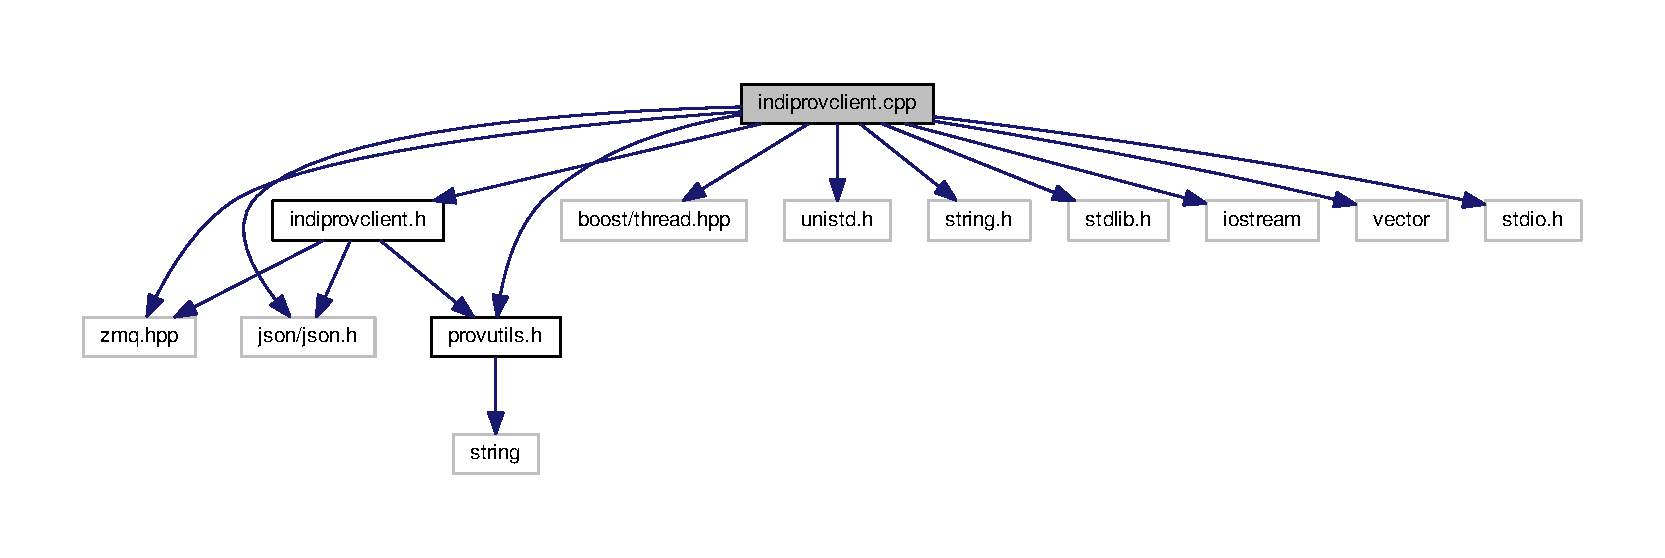
\includegraphics[width=350pt]{indiprovclient_8cpp__incl}
\end{center}
\end{figure}

\hypertarget{indiprovclient_8h}{\section{indiprovclient.\-h File Reference}
\label{indiprovclient_8h}\index{indiprovclient.\-h@{indiprovclient.\-h}}
}
{\ttfamily \#include \char`\"{}zmq.\-hpp\char`\"{}}\\*
{\ttfamily \#include $<$json/json.\-h$>$}\\*
{\ttfamily \#include \char`\"{}provutils.\-h\char`\"{}}\\*
Include dependency graph for indiprovclient.\-h\-:
\nopagebreak
\begin{figure}[H]
\begin{center}
\leavevmode
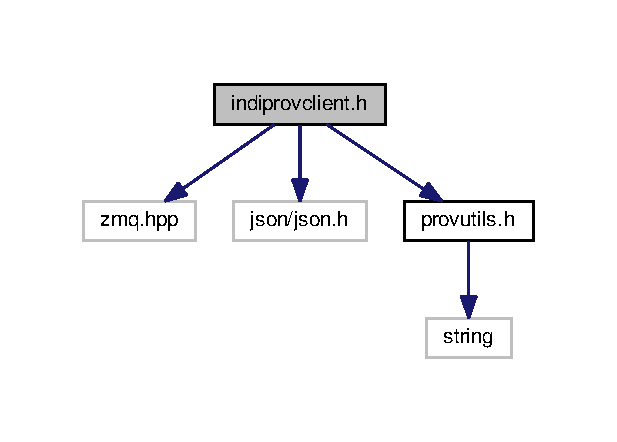
\includegraphics[width=296pt]{indiprovclient_8h__incl}
\end{center}
\end{figure}
This graph shows which files directly or indirectly include this file\-:
\nopagebreak
\begin{figure}[H]
\begin{center}
\leavevmode
\includegraphics[width=279pt]{indiprovclient_8h__dep__incl}
\end{center}
\end{figure}
\subsection*{Classes}
\begin{DoxyCompactItemize}
\item 
class \hyperlink{class_in_di_prov_client}{In\-Di\-Prov\-Client}
\begin{DoxyCompactList}\small\item\em \hyperlink{class_in_di_prov_client}{In\-Di\-Prov\-Client} class. \end{DoxyCompactList}\end{DoxyCompactItemize}

\hypertarget{main_8cpp}{\section{main.\-cpp File Reference}
\label{main_8cpp}\index{main.\-cpp@{main.\-cpp}}
}
{\ttfamily \#include \char`\"{}mainwindow.\-h\char`\"{}}\\*
{\ttfamily \#include $<$Q\-Application$>$}\\*
Include dependency graph for main.\-cpp\-:
\nopagebreak
\begin{figure}[H]
\begin{center}
\leavevmode
\includegraphics[width=335pt]{main_8cpp__incl}
\end{center}
\end{figure}
\subsection*{Functions}
\begin{DoxyCompactItemize}
\item 
int \hyperlink{main_8cpp_a0ddf1224851353fc92bfbff6f499fa97}{main} (int argc, char $\ast$argv\mbox{[}$\,$\mbox{]})
\end{DoxyCompactItemize}


\subsection{Function Documentation}
\hypertarget{main_8cpp_a0ddf1224851353fc92bfbff6f499fa97}{\index{main.\-cpp@{main.\-cpp}!main@{main}}
\index{main@{main}!main.cpp@{main.\-cpp}}
\subsubsection[{main}]{\setlength{\rightskip}{0pt plus 5cm}int main (
\begin{DoxyParamCaption}
\item[{int}]{argc, }
\item[{char $\ast$}]{argv\mbox{[}$\,$\mbox{]}}
\end{DoxyParamCaption}
)}}\label{main_8cpp_a0ddf1224851353fc92bfbff6f499fa97}

\hypertarget{mainwindow_8cpp}{\section{mainwindow.\-cpp File Reference}
\label{mainwindow_8cpp}\index{mainwindow.\-cpp@{mainwindow.\-cpp}}
}
{\ttfamily \#include \char`\"{}mainwindow.\-h\char`\"{}}\\*
{\ttfamily \#include \char`\"{}ui\-\_\-mainwindow.\-h\char`\"{}}\\*
{\ttfamily \#include $<$boost/thread.\-hpp$>$}\\*
{\ttfamily \#include $<$unistd.\-h$>$}\\*
{\ttfamily \#include \char`\"{}zmq.\-hpp\char`\"{}}\\*
{\ttfamily \#include $<$json/json.\-h$>$}\\*
{\ttfamily \#include \char`\"{}indiprovclient.\-h\char`\"{}}\\*
{\ttfamily \#include $<$iostream$>$}\\*
{\ttfamily \#include $<$fstream$>$}\\*
{\ttfamily \#include $<$boost/archive/text\-\_\-oarchive.\-hpp$>$}\\*
{\ttfamily \#include $<$boost/archive/text\-\_\-iarchive.\-hpp$>$}\\*
{\ttfamily \#include $<$boost/serialization/vector.\-hpp$>$}\\*
Include dependency graph for mainwindow.\-cpp\-:
\nopagebreak
\begin{figure}[H]
\begin{center}
\leavevmode
\includegraphics[width=350pt]{mainwindow_8cpp__incl}
\end{center}
\end{figure}
\subsection*{Classes}
\begin{DoxyCompactItemize}
\item 
struct \hyperlink{structmyteststruct}{myteststruct}
\end{DoxyCompactItemize}

\hypertarget{mainwindow_8h}{\section{mainwindow.\-h File Reference}
\label{mainwindow_8h}\index{mainwindow.\-h@{mainwindow.\-h}}
}
{\ttfamily \#include $<$Q\-Main\-Window$>$}\\*
{\ttfamily \#include \char`\"{}zmq.\-hpp\char`\"{}}\\*
{\ttfamily \#include $<$json/json.\-h$>$}\\*
Include dependency graph for mainwindow.\-h\-:
\nopagebreak
\begin{figure}[H]
\begin{center}
\leavevmode
\includegraphics[width=314pt]{mainwindow_8h__incl}
\end{center}
\end{figure}
This graph shows which files directly or indirectly include this file\-:
\nopagebreak
\begin{figure}[H]
\begin{center}
\leavevmode
\includegraphics[width=242pt]{mainwindow_8h__dep__incl}
\end{center}
\end{figure}
\subsection*{Classes}
\begin{DoxyCompactItemize}
\item 
class \hyperlink{class_main_window}{Main\-Window}
\end{DoxyCompactItemize}
\subsection*{Namespaces}
\begin{DoxyCompactItemize}
\item 
\hyperlink{namespace_ui}{Ui}
\end{DoxyCompactItemize}

\hypertarget{msgparsing_8cpp}{\section{msgparsing.\-cpp File Reference}
\label{msgparsing_8cpp}\index{msgparsing.\-cpp@{msgparsing.\-cpp}}
}
{\ttfamily \#include \char`\"{}msgparsing.\-h\char`\"{}}\\*
Include dependency graph for msgparsing.\-cpp\-:
\nopagebreak
\begin{figure}[H]
\begin{center}
\leavevmode
\includegraphics[width=166pt]{msgparsing_8cpp__incl}
\end{center}
\end{figure}

\hypertarget{msgparsing_8h}{\section{msgparsing.\-h File Reference}
\label{msgparsing_8h}\index{msgparsing.\-h@{msgparsing.\-h}}
}
This graph shows which files directly or indirectly include this file\-:
\nopagebreak
\begin{figure}[H]
\begin{center}
\leavevmode
\includegraphics[width=166pt]{msgparsing_8h__dep__incl}
\end{center}
\end{figure}
\subsection*{Classes}
\begin{DoxyCompactItemize}
\item 
class \hyperlink{classmsg_parsing}{msg\-Parsing}
\end{DoxyCompactItemize}

\hypertarget{provutils_8cpp}{\section{provutils.\-cpp File Reference}
\label{provutils_8cpp}\index{provutils.\-cpp@{provutils.\-cpp}}
}
{\ttfamily \#include \char`\"{}provutils.\-h\char`\"{}}\\*
Include dependency graph for provutils.\-cpp\-:
\nopagebreak
\begin{figure}[H]
\begin{center}
\leavevmode
\includegraphics[width=152pt]{provutils_8cpp__incl}
\end{center}
\end{figure}

\hypertarget{provutils_8h}{\section{provutils.\-h File Reference}
\label{provutils_8h}\index{provutils.\-h@{provutils.\-h}}
}
{\ttfamily \#include $<$string$>$}\\*
Include dependency graph for provutils.\-h\-:
\nopagebreak
\begin{figure}[H]
\begin{center}
\leavevmode
\includegraphics[width=140pt]{provutils_8h__incl}
\end{center}
\end{figure}
This graph shows which files directly or indirectly include this file\-:
\nopagebreak
\begin{figure}[H]
\begin{center}
\leavevmode
\includegraphics[width=326pt]{provutils_8h__dep__incl}
\end{center}
\end{figure}
\subsection*{Classes}
\begin{DoxyCompactItemize}
\item 
class \hyperlink{class_prov_utils}{Prov\-Utils}
\item 
struct \hyperlink{struct_prov_utils_1_1_entity}{Prov\-Utils\-::\-Entity}
\item 
struct \hyperlink{struct_prov_utils_1_1_activity}{Prov\-Utils\-::\-Activity}
\item 
struct \hyperlink{struct_prov_utils_1_1_agent}{Prov\-Utils\-::\-Agent}
\item 
struct \hyperlink{struct_prov_utils_1_1_used}{Prov\-Utils\-::\-Used}
\item 
struct \hyperlink{struct_prov_utils_1_1_was_generated_by}{Prov\-Utils\-::\-Was\-Generated\-By}
\item 
struct \hyperlink{struct_prov_utils_1_1_was_derived_from}{Prov\-Utils\-::\-Was\-Derived\-From}
\item 
struct \hyperlink{struct_prov_utils_1_1_was_attributed_to}{Prov\-Utils\-::\-Was\-Attributed\-To}
\item 
struct \hyperlink{struct_prov_utils_1_1_was_associated_with}{Prov\-Utils\-::\-Was\-Associated\-With}
\item 
struct \hyperlink{struct_prov_utils_1_1_was_started_by}{Prov\-Utils\-::\-Was\-Started\-By}
\item 
struct \hyperlink{struct_prov_utils_1_1_was_ended_by}{Prov\-Utils\-::\-Was\-Ended\-By}
\item 
struct \hyperlink{struct_prov_utils_1_1_was_informed_by}{Prov\-Utils\-::\-Was\-Informed\-By}
\end{DoxyCompactItemize}

%--- End generated contents ---

% Index
\newpage
\phantomsection
\addcontentsline{toc}{chapter}{Index}
\printindex

\end{document}
